% 150 câu đã gỡ khỏi ngân hàng (chuyen_dang) — chép lại vào file dạng để khôi phục

% từ: cau-hoi/lop10/0D0_Xac_suat/0D0-1-3_Dem_phan_tu_khong_gian_mau_bien_co.tex
\begin{ex}%[0D0N1-3]%[0D0H1-3]%[0D0K1-3]%[ma:73818f64]
	 Cho các chữ số $0$, $ 2 $, $ 3 $, $ 6 $, $ 7 $.
	\choiceTF 
		{\True Chọn ngẫu nhiên một chữ số, xác xuất để được chữ số $0$ là  $\dfrac{1}{5}$}
		{Chọn ngẫu nhiên một chữ số, số khả năng  thuận lợi để được chữ số là hợp số là $1$}
		{\True Số các số có $2$ chữ số khác nhau chia hết cho $3$ lập được  từ các chữ số đã cho là $5$}
		{\True Có $18$ số có $3$ chữ số khác nhau lập được từ các chữ số đã cho chia  hết cho $4$}
	 \loigiai{
		\begin{itemize}
			\item 
			Số phần tử của  không gian mẫu là $5$.\\
			Số khả  năng thuận lợi để chọn được chữ số $0$ là $1$.\\
			Do  đó,
			xác suất để được chữ số $0$ là $\dfrac{1}{5}$. 
			\item 
			Trong $5$ chữ số đã cho có $2$ hợp số là số $0$ và  $6$.\\
			Do đó, số khả năng thuận lợi để được chữ số  là hợp số là $2$.
			\item Các số có hai chữ số khác nhau chia  hết cho $3$ lập được từ các chữ số đã cho là
			$$27,\  30,\ 36,\ 60,\, 63,\ 72.$$
			Vậy có $6$ số có hai  chữ số khác nhau chia hết cho $3$.
			\item Gọi $\overline{abc}$ là số có $3$  chữ số khác nhau chia hết cho $4$.\\
			Ta có $\overline{bc}$ chia hết cho $4$  nên $\overline{bc}\in \{20;32;36;60;72;76\}$.\\
			Do đó: $\overline{bc}$ có $6$ cách chọn và ứng với mỗi $\overline{bc}$ đã chọn thì $a$ có $3$  cách chọn.\\
			Vậy số các số có $3$ chữ số khác nhau lập được từ các chữ số đã  cho chia hết cho $4$ là $6\cdot 3=18$ (số).
		\end{itemize}
		\begin{itemchoice}
			 \itemch Đúng.
			\itemch  Sai.
			\itemch  Sai.
			\itemch  Đúng.
		\end{itemchoice}
	} 
\end{ex}

% từ: cau-hoi/lop10/0D0_Xac_suat/0D0-2-2_Lien_quan_xuc_xac_dong_tien_PP_liet_ke.tex
\begin{ex}%[0D0H2-2]%[ma:d88157e6]
	Xét phép thử $T$: \lq\lq Tung một con xúc xắc cân đối và đồng chất\rq\rq\, và biến cố $A$: \lq\lq Số  chấm xuất hiện bé hơn $5$\rq\rq.
	\choiceTF 
		{\True  Không gian mẫu $\Omega=\{1;2;3;4;5;6\}$}
		{Số kết quả thuận lợi cho  biến cố $A$ là $5$}
		{Biến cố $\overline{A}$ là biến cố \lq\lq Số chấm  xuất hiện lớn hơn $5$\rq\rq}
		 {Xác xuất của biến cố $\overline{A}$ là $\mathrm{P}(\overline{A})=\dfrac{1}{6}$}
	 \loigiai{
		\begin{itemchoice}
			\itemch  Không gian mẫu $\Omega=\{1;2;3;4;5;6\}$.
			\itemch Ta có $A=\{1;2;3;4\}$ nên có $4$ kết quả  thuận lợi cho biến cố $A$.
			\itemch Biến cố $\overline{A}$ là biến cố \lq\lq  Số chấm xuất hiện lớn hơn hoặc bằng $5$\rq\rq\,.
			 \itemch Vì $\mathrm{P}(A)=\dfrac{4}{6}=\dfrac{2}{3}$ nên $\mathrm{P}(\overline{A})=1-\dfrac{2}{3}=\dfrac{1}{3}$.
		\end{itemchoice}
	} 
\end{ex}

% từ: cau-hoi/lop10/0D1_Menh_de_Tap_hop/0D1-1-3_Phu_dinh_cua_mot_menh_de.tex
\begin{ex}%[0D1B1-3]%[ma:20e12e16]
	 Cho mệnh đề "Phương trình $x^2+2x+1=0$ có nghiệm". Tìm mệnh đề phủ định của mệnh đề trên và cho biết tính đúng sai của mệnh đề phủ định.
	\choice 
		{``Phương trình $x^2+2x+1=0$ có hai nghiệm phân  biệt''. Đây là mệnh đề sai}
		{``Phương trình $x^2+2x+1=0$ có  nghiệm kép''. Đây là mệnh đề đúng}
		{\True  ``Phương trình $x^2+2x+1=0$ vô nghiệm''. Đây là mệnh đề sai}
		{``Phương trình $x^2+2x+1=0$ vô nghiệm''. Đây  là mệnh đề đúng}
	\loigiai{Mệnh đề phủ định là ``Phương trình $x^2+2x+1=0$  vô nghiệm.''\\
	Rõ ràng phương trình này có nghiệm $x=-1$ nên  mệnh đề này sai.}
\end{ex}

% từ: cau-hoi/lop10/0D1_Menh_de_Tap_hop/0D1-1-3_Phu_dinh_cua_mot_menh_de.tex
\begin{bt}%[0D1V1-3]%[ma:cf8fa871]
	Cho mệnh đề  $P: \forall n\in N: n > \dfrac{1}{n}$. Gọi $S$ là tập hợp các phần tử $n$ để mệnh đề $\overline{P}$ đúng. Tìm số phần tử của tập $S$.
	\loigiai{ 
		Ta có 
		\[\overline{P}: \exists  n\in N: n\le \dfrac{1}{n}
		\] 
		Vì $n\in N$ nên bất phương trình  xác định khi $n > 0$ hay $n\ge 1$. Ta có $n\le \dfrac{1}{n} \Leftrightarrow n^2\le 1\Leftrightarrow n\le 1$.\\
		Kết hợp  điều kiện ta có $1\le n\le 1\Rightarrow n=1$.\\
		 Vậy tập $S$ có đúng $1$ phần tử.
	} 
\end{bt}

% từ: cau-hoi/lop10/0D1_Menh_de_Tap_hop/0D1-1-4_Menh_de_keo_theo_menh_de_dao_menh_de_tuong_du.tex
\begin{ex}%[0D1B1-4]%[ma:79b43f5e]
	Trong các  mệnh đề sau, mệnh đề nào là đúng?
	 \choice
		 {Tổng của hai số tự nhiên là một số chẵn khi và chỉ khi cả hai số đều là số chẵn}
		 {Tích của hai số tự nhiên là một số chẵn khi và chỉ khi cả hai số đều là số chẵn}
		{Tổng của hai số tự nhiên là một số  lẻ khi và chỉ khi cả hai số đều là số lẻ}
		{\True Tích của hai số tự nhiên là một số  lẻ khi và chỉ khi cả hai số đều là số lẻ}
	 \loigiai{
		Ta có các nhận  xét sau đây:
		\begin{itemize}
			\item Hai số lẻ vẫn  có tổng là số chẵn.
			\item Chỉ cần ít  nhất một thừa số chẵn thì tích hai số là số chẵn.
			\item Tổng hai số tự nhiên lẻ lại là một số  chẵn.
			\item Tích hai số  tự nhiên lẻ thì trong các thừa số không có thừa số chẵn, hay nói cách khác tất cả các thừa số đều là số lẻ.
		\end{itemize}
	 }
\end{ex}

% từ: cau-hoi/lop10/0D1_Menh_de_Tap_hop/0D1-1-4_Menh_de_keo_theo_menh_de_dao_menh_de_tuong_du.tex
\begin{ex}%[0D1B1-4]%[ma:b0182ed8]
	Cho các  mệnh đề sau:
	\begin{multicols}{2}
		\begin{enumerate}
			 \item ``Tam giác $ABC$ đều'';
			\item ``Tam giác $ABC$  có 2 góc bằng $60^\circ$'';
			\item ``Tam giác $ABC$  cân'';
			 \item ``$\triangle ABC$ có ba cạnh $AB=AC=BC$''.
		\end{enumerate}
	\end{multicols}
	Hỏi có bao nhiêu cặp mệnh đề  tương đương?
	\choice 
		{\True $3$} 
		{$2$} 
		{$6$} 
		 {$4$}
	\loigiai{ 
		Ta có $ P\Leftrightarrow Q $, $ Q\Leftrightarrow S $ và  $ S\Leftrightarrow P $.
	} 
\end{ex}

% từ: cau-hoi/lop10/0D1_Menh_de_Tap_hop/0D1-2-2_Tap_hop_con_Hai_tap_hop_bang_nhau.tex
\begin{ex}%[0D1H2-2]%[ma:0c598e10]
	Cho các tập hợp $A=\{-3;-2;-1; 0; 1; 2;  3\}$, $B=\{0; 1; 4; 5\}$ và $C=\{-4;-3; 1; 2; 5; 6\}$.
	 \choiceTF
		 {\True $A\cup B=\{-3;-2;-1; 0; 1; 2; 3; 4; 5\}$}
		{$A\cap  B=\{0\}$}
		{\True  $(A\cup B)\cap C=\{-3; 1; 2; 5\}$}
		{\True $A\cap B\cap  C=\{1\}$}
	\loigiai{ 
		\begin{itemchoice}
			\itemch Vì $A\cup B=\{-3;-2;-1; 0;  1; 2; 3; 4; 5\}$.
			\itemch Vì  $A\cap B=\{0; 1\}$.
			\itemch Vì $(A\cup  B)\cap C=\{-3; 1; 2; 5\}$.
			 \itemch Vì $A\cap B\cap C=\{1\}$.
		\end{itemchoice}
	 }
\end{ex}

% từ: cau-hoi/lop10/0D2_BPT_va_he_BPT_bac_nhat_hai_an/0D2-2-2_Mien_nghiem_cua_He_BPT_bac_nhat_hai_an.tex
\begin{bt}%[0D2H2-2]%[Tex hóa SGK CD-CT,T7/22, Đoàn Minh Tân]%[ma:23a0d4bd]
	\immini{Trên miền đa giác không gạch chéo ở hình bên, hãy
		\begin{enumerate}
			\item tìm GTLN của $F=2x+3y$.
			\item tìm GTNN của $G=x-4y$.
		\end{enumerate}
	}
	{
		\begin{tikzpicture}[scale=0.7, x=5mm, y=5mm, font=\footnotesize, line join=round, line cap=round,>=stealth]
			\def \xmin{-2};
			\def \xmax{12};
			\def \ymin{-2};
			\def \ymax{17};
			\draw[->] (\xmin, 0.) -- (\xmax,0.) node[anchor=north] {$x$};
			\draw[->] (0.,\ymin) -- (0.,\ymax) node[anchor=west] {$y$};
			\clip(\xmin-0.1,\ymin-0.1) rectangle (\xmax+0.1,\ymax+0.1);
			\fill[pattern=north east lines,opacity=0.4] (-2/3,17) plot[smooth,domain=-2:12] (\x,{-3*(\x)+15})--(12,-2)--(12,17)--cycle;
			\draw[smooth] plot[domain=\xmin:\xmax] (\x,{-3*(\x)+15});
			\fill[pattern=north west lines, opacity=0.4] (-2,7.5) plot[smooth,domain=-2:12] (\x,{(24-3*(\x))/4}) (32/3,-2)--(12,-2)--(12,17)--(-2,17)--(-2,7.5);
			\draw[smooth] plot[domain=\xmin:\xmax] (\x,{(24-3*(\x))/4});
			\fill[pattern=vertical lines,opacity=0.4] (-2,0)--(12,0)--(12,-2)--(-2,-2)--cycle;
			\fill[pattern= horizontal lines,opacity=0.4] (-2,-2)--(0,-2)--(0,17)--(-2,17)--cycle;
			\draw[fill=black] (0,0) circle (1pt) node[below right] {$O$} (5,0) circle(1pt) node[below]{$5$} node[above left]{$(5;0)$} (10,0) circle(1pt) node[above]{$10$} (4,3) circle(1pt) node[right]{$(4;3)$} (0,5) node[left]{$5$} (0,10) circle(1pt) node[left]{$10$} (0,15) circle(1pt) node[left]{$15$} (0,6) circle(1pt) node[right]{$(0;6)$};
		\end{tikzpicture}
	}
	\loigiai{
		Miền nghiệm là tứ giác $OABC$ với $O(0;0)$, $A(5{,}0)$, $B(4;3)$, $C(0;6)$.
		\begin{enumerate}
			\item Xét $F=2x+3y$
			Tại $O(0;0)$, $F=0$; tại $A(5;0)$, $F=10$, tại $B(4;3)$, $F=17$, tại $C(0;6)$, $F=18$.\\
			Vậy $F$ đạt giá trị lớn nhất là $18$ tại điểm $C(0;6)$.
			\item Xét $G=x-4y$.\\
			Tại $O(0;0)$, $G=0$; tại $A(5;0)$, $F=5$, tại $B(4;3)$, $F=-8$, tại $C(0;6)$, $F=-24$.\\
			Vậy $G$ đạt giá trị nhỏ nhât là $-24$ tại $C(0;6)$.
		\end{enumerate}
	}
\end{bt}

% từ: cau-hoi/lop10/0D3_Ham_so_bac_hai_va_do_thi/0D3-1-2_Tap_xac_dinh_cua_ham_so.tex
\begin{ex}%[0D3Y1-2]%[ma:519454e6]
	Gieo con súc sắc $2$ lần. Biến cố nào dưới  đây là biến cố tổng số chấm trong hai lần gieo bằng $7$?
	\choice 
		 {\True $A=\left\{(1;6),(6;1),(3;4),(4;3),(5;2),(2;5)\right\}$}
		{$B=\left\{(1;6),(3;4),(5;2)\right\}$} 
		 {$C=\left\{(1;6),(6;1),(3;4),(4;3)\right\}$}
		{$D=\left\{(2;6),(6;2),(3;4),(4;3),(5;2),(2;5)\right\}$} 
	\loigiai{ 
		Ta  có $A=\left\{(1;6),(6;1),(3;4),(4;3),(5;2),(2;5)\right\}$.
	} 
\end{ex}

% từ: cau-hoi/lop10/0D3_Ham_so_bac_hai_va_do_thi/0D3-1-2_Tap_xac_dinh_cua_ham_so.tex
\begin{bt}%[0D3N1-2]%[Dự án đề kiểm tra HKI NH22-23-Mui Doan]%[THPT Nguyễn An Ninh-Sở Hồ Chí Minh]%[ma:5fffb6ec]
	\immini{
		Cho hàm số $y=f(x)$ có đồ thị như hình vẽ bên dưới
		\begin{listEX}
			\item Tìm tập xác định và tập giá trị của hàm số.
			\item Tính $f(-1)$, $f(6)$.
		\end{listEX}
	}{
		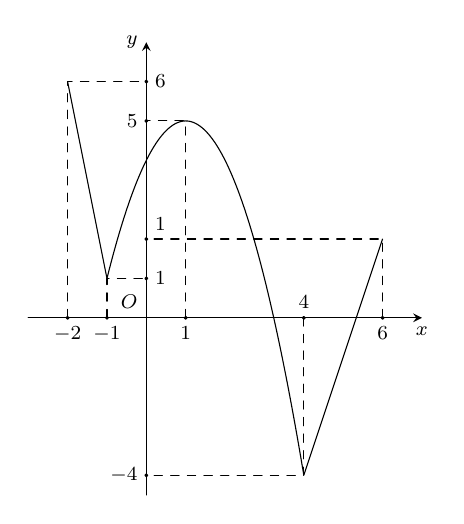
\begin{tikzpicture}[scale=0.5,>=stealth, font=\footnotesize, line join=round, line cap=round]
			\def\a{-1} \def\b{2} \def\c{4} % Hệ số
			\def\xmin{-3} \def\xmax{7}
			\def\ymin{-4.5} \def\ymax{7} 
			%	\draw[color=gray!50,dashed] (\xmin,\ymin) grid (\xmax,\ymax); 
			\draw[->] (\xmin,0)--(\xmax,0) node [below]{$x$};
			\draw[->] (0,\ymin)--(0,\ymax) node [left]{$y$};
			\node at (0,0) [above left]{$O$};
			\clip (\xmin+0.1,\ymin+0.1) rectangle (\xmax-0.5,\ymax-0.1);
			\draw[smooth,samples=300,domain=-1:4] plot(\x,{\a*(\x)^2+\b*(\x)+\c});
			\draw[dashed] (-2,0)|-(0,6) (-1,0)|-(0,1) (1,0)|-(0,5) (4,0)|-(0,-4) (6,0)|-(0,2);
			\draw (-2,6)--(-1,1) (4,-4)--(6,2);
			\draw[fill=black]
			(-2,0)node[below]{$-2$}circle(1pt)
			(-1,0)node[below]{$-1$}circle(1pt)
			(1,0)node[below]{$1$}circle(1pt)
			(6,0)node[below]{$6$}circle(1pt)
			(4,0)node[above]{$4$}circle(1pt)
			(0,6)node[right]{$6$}circle(1pt)
			(0,5)node[left]{$5$}circle(1pt)
			(0,-4)node[left]{$-4$}circle(1pt)
			(0,1)node[right]{$1$}circle(1pt)
			(0,2)node[above right]{$1$}circle(1pt);
		\end{tikzpicture}
	}
	\loigiai{
		\begin{listEX}
			\item Tập xác định $\mathscr{D}=[-2;6]$; tập giá trị $I=[-4;6]$.
			\item $f(-1)=1$, $f(6)=2$.
		\end{listEX}
	}
\end{bt}

% từ: cau-hoi/lop10/0D3_Ham_so_bac_hai_va_do_thi/0D3-1-3_Gia_tri_cua_ham_so.tex
\begin{ex}%[0D3N1-3]%[ma:f09216c5]
	Hàm số $f(x)=\heva{&\dfrac{2\sqrt{x-2}-3}{x-1}, &\text{~khi~}  \, x\ge 2\\&x^2+2, &\text{~khi~} \, x < 2}$. Tính $P=f(2)+f(-2)$.
	 \choice
		 {\True $P=3$}
		 {$P=\dfrac{7}{3}$}
		{$P=6$} 
		{$P=2$} 
	\loigiai{ 
		Khi $x=2$  thì $f(x)=\dfrac{2\sqrt{x-2}-3}{x-1}$.\\
		Khi  $x=-2$ thì $f(x)=x^2+2$.\\
	Từ đó  ta có $P=f(2)+f(-2)=\dfrac{2\sqrt{2-2}-3}{2-1}+(-2)^2+2=3$.}
\end{ex}

% từ: cau-hoi/lop10/0D3_Ham_so_bac_hai_va_do_thi/0D3-1-4_Do_thi_cua_ham_so.tex
\begin{ex}%[0D3H1-4]%[ma:254341cb]
	\immini{Cho hàm số $y=f(x)$  có đồ thị như hình vẽ bên. Mỗi kết quả dưới đây đúng hay sai?}{
	\begin{tikzpicture}[font=\footnotesize,line join=round,line cap=round,>=stealth,scale=1]
			\draw[->]  (-2,0) -- (2,0) node[below] {$x$};
			\draw[->] (0,-2.2) --  (0,2.5) node[left] {$y$};
			\begin{scope}
				\clip (-2.5,-2.5)  rectangle (3,2);
				\draw[samples=200,domain=-2: 5,smooth,variable=\x] plot (\x,{(\x)^4-2*(\x)^2-1}); 
			\end{scope}
			 \draw[dashed] (1,0)--(1,-2)--(-1,-2)--(-1,0);
			\foreach \x/\y  in{0/0,1/0,-1/0,0/-1,0/-2,1/-2,-1/-2}{
				 \fill (\x,\y) circle (1.5pt);
			 }
			\path 
				node  at (0,0)[above left]{$O$}
				node  at (1,0)[below left]{$1$}
				node  at (-1,0)[above]{$-1$}
				node at (0,-1)[above left]{$-1$} 
				 node at (0,-2)[above left]{$-2$};
		\end{tikzpicture}
	 }
	 \choiceTF
		{Phương trình $f(x)=0$ có  $4$ nghiệm phân biệt}
		{\True $f(2)=f(-2)$} 
		{\True Hàm số nghịch  biến trên $\left(0;1\right)$}
		{\True $-2\le f(x)$, $\forall  x\in\mathscr{D}$}
	\loigiai{ 
		\begin{itemchoice}
			\itemch Đồ thị  hàm số $y=f(x)$ cắt trục hoành tại hai điểm có hoành độ $x=0$ và $x=1$.
			\itemch Từ đồ thị hàm số  $y=f(x)$ thì $f(0)=0$.
			\itemch Từ đồ thị của hàm số suy ra hàm số  đồng biến trên $\left(-\infty;0\right)$.
			\itemch Từ đồ thị ta  có $f(x)<1$.
		\end{itemchoice}
	 }
\end{ex}

% từ: cau-hoi/lop10/0D3_Ham_so_bac_hai_va_do_thi/0D3-1-5_Tinh_dong_bien_nghich_bien.tex
\begin{ex}%[0D3B1-5]%[ma:d4d63084]
	 \immini{
	Cho hàm số có đồ thị như hình bên. Khẳng định nào sau  đây là đúng?
	 \choice
		{Hàm số  nghịch biến trên khoảng $(0;3)$}
		 {Hàm số đồng biến trên khoảng $(-\infty;3)$}
		{Hàm số đồng biến trên  khoảng $(-\infty;1)$}
		{\True Hàm số nghịch biến trên khoảng  $(0;2)$}}
		{\vspace{-0.5cm} 
		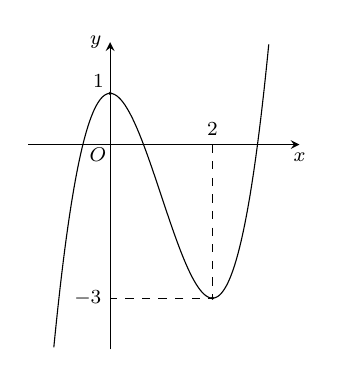
\begin{tikzpicture}[scale=0.65,font=\footnotesize,samples=200,>=stealth]
				\draw[->] (-1.6,0)--(3.7,0) node[below]{$x$}; 
				 \draw[->] (0,-4)--(0,2) node[left]{$y$};
				\node at (0,0)  [below left=-2pt]{$O$};
				\draw plot[domain=-1.1:3.1]  (\x,{(\x)^3-3*(\x)^2+1});
				 \fill
					(0,1) circle (1pt) node[above  left=-1pt]{$1$}
					(2,-3)  circle (1pt);
				 \draw[dashed]
					(2,0) node[above]{$2$} |-(0,-3)  node[left]{$-3$};
			\end{tikzpicture}
		} 
	\loigiai{ 
		Hình bên có đồ thị của hàm số đồng biến trên các khoảng $(-\infty;0)$, $(2;+\infty)$ và nghịch biến trên khoảng  $(0;2)$.
	 }
\end{ex}

% từ: cau-hoi/lop10/0D3_Ham_so_bac_hai_va_do_thi/0D3-1-5_Tinh_dong_bien_nghich_bien.tex
\begin{bt}%[0D3C1-5]%[Dự án Tex Toán 10 chương trình mới]%[ma:4197311b]
	Tìm các giá trị của $m$ để hàm số $y=\dfrac{mx}{x-1}$ đồng biến trên $(1;+\infty)$.
	\loigiai{
		Với $1<x_1<x_2$, ta có: $y_1-y_2=\dfrac{m(x_2-x_1)}{(x_1-1)(x_2-1)}$. Mà $y_1-y_2<0\Rightarrow m<0$.
	}
\end{bt}

% từ: cau-hoi/lop10/0D3_Ham_so_bac_hai_va_do_thi/0D3-1-5_Tinh_dong_bien_nghich_bien.tex
\begin{bt}%[0D3N1-5]%[Dự án đề kiểm tra HKI NH22-23- Hieu Phan]%[THPT Tây Thạnh]%[ma:5d4df42d]
\immini{
Cho hàm số $y=f(x)$ xác định trên $[-2 ; 6]$ và có đồ thị như hình dưới đây. Tìm các khoảng đồng biến, nghịch biến của hàm số $y=f(x)$.
}{
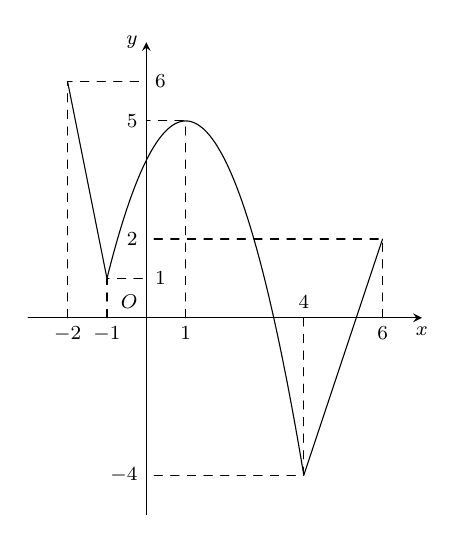
\begin{tikzpicture}[scale=0.5,>=stealth, font=\footnotesize, line join=round, line cap=round]
\def\a{-1} \def\b{2} \def\c{4} % Hệ số
\def\xmin{-3} \def\xmax{7}
\def\ymin{-5} \def\ymax{7}
%\draw[color=gray!50,dashed] (\xmin,\ymin) grid (\xmax,\ymax);
\draw[->] (\xmin,0)--(\xmax,0) node [below]{$x$};
\draw[->] (0,\ymin)--(0,\ymax) node [left]{$y$};
\node at (0,0) [above left]{$O$};
\draw[dashed] (-2,0)node [below]{$-2$}--(-2,6)--(0,6)node [right]{$6$};
\draw[dashed] (-1,0)node [below]{$-1$}--(-1,1)--(0,1)node [right]{$1$};
\draw[dashed] (1,0)node [below]{$1$}--(1,5)--(0,5)node [left]{$5$};
\draw[dashed] (4,0)node [above]{$4$}--(4,-4)--(0,-4)node [left]{$-4$};
\draw[dashed] (6,0)node [below]{$6$}--(6,2)--(0,2)node [left]{$2$};
\draw (4,-4)--(6,2) (-2,6)--(-1,1);
\clip (\xmin+0.1,\ymin+0.1) rectangle (\xmax-0.5,\ymax-0.1);
\draw[smooth,samples=300][domain=-1:4] plot(\x,{\a*(\x)^2+\b*(\x)+\c});
\end{tikzpicture}
}
\loigiai{
Dựa vào đồ thị ta suy ra 
\begin{itemize}
    \item Các khoảng đồng biến là $(-1;1)$, $(4;6)$;
    \item Các khoảng nghịch biến là $(-2;-1)$, $(1;4)$.
\end{itemize} 
}
\end{bt}

% từ: cau-hoi/lop10/0D3_Ham_so_bac_hai_va_do_thi/0D3-1-5_Tinh_dong_bien_nghich_bien.tex
\begin{bt}%[0D3H1-5] %[Dự án đề kiểm tra HKII NH22-23 - Nguyên Huỳnh]%[THPT Tam Phú]%[ma:6564aba6]
	\immini{	Cho hàm số $y = f(x)$ có đồ thị trên $[-2; 3]$ như sau. 	\begin{enumerate}
			\item[a)] Lập bảng biến thiên của hàm số trên $[-2; 3]$.
			\item[b)] Cho biết giá trị lớn nhất và giá trị nhỏ nhất của hàm số trên $[0; 3]$.
	\end{enumerate}}
	{
		\begin{tikzpicture}[line join = round, line cap = round,>=stealth,font=\footnotesize,scale=0.7]
			\def\xt{-3} \def\xp{4} \def\yd{-4} \def\yt{3} ;
			\draw[->] (\xt,0)--(\xp,0) node[above]{$x$};
			\draw[->] (0,\yd)--(0,\yt) node[left]{$y$};
			\draw[dashed,thin,black] (-2,0)--(-2,2)--(0,2);
			\draw[dashed,thin,black] (0,1)--(1,1)--(1,0);
			\draw[dashed,thin,black] (3,0)--(3,-3)--(0,-3);
			\fill (0,0) circle (1.5pt) node[below left]{$O$} (-2,0) circle (1.5pt) node[below]{$-2$} (-1,0) circle (1.5pt)  (1,0) circle (1.5pt) node[below]{$1$} (2,0) circle (1.5pt) node[below left]{$2$} (3,0) circle (1.5pt) node[above]{$3$} (0,-3) circle (1.5pt) node[left]{$-3$} (0,-1) circle (1.5pt) node[left]{$-1$} (0,1) circle (1.5pt) node[left]{$1$} (0,2) circle (1.5pt) node[right]{$2$};
			\begin{scope}
				\clip (-2,0) rectangle (0,2);
				\draw[samples=150,thick,smooth,domain=\xt:\xp] plot(\x,{-\x});
			\end{scope}
			\begin{scope}
				\clip (0,-3) rectangle (3,1);
				\draw[samples=150,thick,smooth,domain=\xt:\xp] plot(\x,{-(\x)^2 + 2*\x});
			\end{scope}
		\end{tikzpicture}
	}
	
	\loigiai{
		\begin{enumerate}
			\item[a)] Ta có bảng biến thiên của hàm số $y = f(x)$ trên $[-2; 3]$ như sau
			\begin{center}
				
\begin{tikzpicture}[line join = round, line cap = round,>=stealth,font=\footnotesize,scale=1]
					\tkzTabInit[nocadre=false,lgt=1,espcl=2.5,deltacl=0.5]{$x$/1,$y$/2}
					{$-2$ , $0$ , $1$ , $3$}
					\tkzTabVar{+/$2$ , -/$0$ , +/$1$ , -/$-3$}
				\end{tikzpicture}
			\end{center}
			\item[b)] Trên đoạn $[0; 3]$ giá trị lớn nhất của hàm số là 2, giá trị nhỏ nhất của hàm số là $-3$.
		\end{enumerate}
	}
\end{bt}

% từ: cau-hoi/lop10/0D3_Ham_so_bac_hai_va_do_thi/0D3-2-1_Xac_dinh_ham_so_bac_hai.tex
\begin{ex}%[0D3Y2-1]%[ma:d7cb2a9a]
	Gieo $2$ con súc sắc cân  đối và đồng chất. Xác suất để tổng số chấm xuất hiện trên hai mặt của $2$
	con súc  sắc đó không vượt quá $5$ là
	 \choice
		{$\dfrac{2}{34}$} 
		 {$\dfrac{7}{18}$}
		 {$\dfrac{8}{9}$}
		 {\True $\dfrac{5}{18}$}
	 \loigiai{
		Ta có  $n(\Omega)=36$.\\
		Biến cố $A$ \lq\lq Tổng số chấm xuất hiện trên hai mặt của  hai con súc sắc không quá $5$\rq\rq.\\
		$A=\left\{(1;1),(1;2);(1;3);(1;4);(2;1);(2;2);(2;3);(3;1);(3;2);(4;1)\right\}$, suy ra $n(A)=10$.\\ 
		Vậy xác suất  biến cố $A$ là $\mathrm{P}(A)=\dfrac{n(A)}{n(\Omega)}=\dfrac{10}{36}=\dfrac{5}{18}$.
	 }
\end{ex}

% từ: cau-hoi/lop10/0D3_Ham_so_bac_hai_va_do_thi/0D3-2-4_Bai_toan_ve_su_tuong_giao.tex
\begin{ex}%[0D3B2-4]%[ma:4abc7234]
	Một hộp chứa ba quả cầu trắng và hai quả cầu đen. Lấy ngẫu nhiên đồng thời hai quả cầu. Xác suất  để lấy được cả hai quả cầu trắng là
	\choice 
		{$\dfrac{4}{10}$} 
		 {\True $\dfrac{3}{10}$}
		{$\dfrac{2}{10}$} 
		{$\dfrac{5}{10}$} 
	\loigiai{ 
		Lấy ngẫu nhiên đồng thời hai quả cầu  từ hộp chứa $3$ quả cầu trắng và $2$ quả cầu đen, số kết quả có thể xảy ra là $n(\Omega)=\mathrm{C}_5^2=10$.\\
		Xét biến cố $A$: ``lấy được $2$ quả cầu trắng''.\\ 
		Số kết quả thuận lợi cho $A$ là $n(A)=\mathrm{C}_3^2=3$, do đó $\mathrm{P}(A)=\dfrac{n(A)}{n(\Omega)}=\dfrac{3}{10}$. 
	} 
\end{ex}

% từ: cau-hoi/lop10/0D3_Ham_so_bac_hai_va_do_thi/0D3-2-4_Bai_toan_ve_su_tuong_giao.tex
\begin{ex}%[0D3Y2-4]%[ma:245c3455]
	Từ một hộp chứa $5$ quả cầu trắng, $6$ quả cầu đỏ, $7$ quả cầu vàng, các quả cầu có kích thước và khối lượng giống nhau, lấy ngẫu nhiên đồng thời $3$ quả cầu. Xác suất lấy được $3$ quả cầu có  ba màu khác nhau là
	 \choice
		 {$\dfrac{35}{68}$}
		{\True $\dfrac{35}{136}$} 
		{$\dfrac{11}{24}$} 
		{$\dfrac{11}{36}$} 
	 \loigiai{
		 Ta có $n\left(\Omega\right)=\mathrm{C}_{18}^3$.\\
		Gọi $A$ là biến  cố \lq\lq lấy được $3$ quả cầu có ba màu khác nhau \rq\rq.\\
		Suy ra $n\left(A\right)=5\cdot  6\cdot 7$.\\
		Do đó  $\mathrm{P}(A)=\dfrac{n(A)}{n(\Omega)}=\dfrac{35}{136}$.
	} 
\end{ex}

% từ: cau-hoi/lop10/0D3_Ham_so_bac_hai_va_do_thi/0D3-2-6_Toan_thuc_te_ung_dung_ham_so_bac_hai.tex
\begin{bt}%[0D3V2-6]%[ma:652e517c]
	Bác Hùng dùng $200$ m hàng rào dây thép gai để rào miếng đất đủ rộng thành một mảnh vườn hình chữ nhật.
	\begin{enumerate}
		\item Tìm công thức tính diện tích $S(x)$ của mảnh vườn hình chữ nhật rào được theo chiều rộng $x$ (m) của mảnh vườn đó.
		\item Tìm kích thước của mảnh vườn hình chữ nhật có diện tích lớn nhất có thể rào được.
	\end{enumerate}
	\loigiai
	{
		\begin{enumerate}
			\item Chiều dài của mảnh vườn là: $100-x(m)$.\\
			Do đó, ta có công thức diện tích $S(x)=(100-x) x=-x^2+100 x~\left(\text{m}^2\right)$.
			\item Mảnh vườn hình chữ nhật có diện tích lớn nhất khi hàm số $S(x)=-x^2+100 x$ đạt giá trị lớn nhất. Vì $a=-1<0$ nên hàm số bậc hai này đạt giá trị lớn nhất tại $x=-\dfrac{b}{2 a}=50$.\\
			Vậy mảnh vườn có diện tích lớn nhất khi nó có kích thước là $50 \text{ m } \times 50 \text{ m}$ (tức là khi nó trở thành hình vuông).
		\end{enumerate}
	}
\end{bt}

% từ: cau-hoi/lop10/0D7_Bat_phuong_trinh_bac_2_mot_an/0D7-1-3_Bai_toan_xet_dau_biet_BXD_do_thi.tex
\begin{ex}%[0D7N1-3]%[ma:2af042bc]
	 \immini{
	Cho hàm số $f(x)=ax^{2}+bx+c$ có đồ thị như hình vẽ. Tìm tất cả giá trị của $x$  để $f(x)<0$.
	\choice 
		{$x\in(-\infty;1)\cup(3;+\infty)$} 
		{\True $x\in(1;3)$} 
		{$x\in(0;2)$} 
		 {$x\in(-1;0)$}
		 }{
		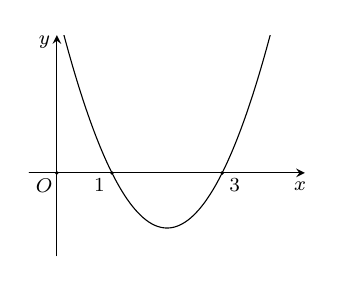
\begin{tikzpicture}[scale=0.7,font=\footnotesize,line join=round,line cap=round,>=stealth]
				\def  \xmin{-.5}
				\def \xmax{4.5} 
				 \def \ymin{-1.5}
				\def  \ymax{2.5}
				\draw[->]  (\xmin,0)--(\xmax,0) node[shift=(-110:0.2)] {$x$};
				\draw[->] (0,\ymin)--(0,\ymax) node[shift=(-150:0.2)]  {$y$};
				 \fill (0,0) circle (1pt) node[shift=(-135:0.25)]{$O$}
					 (1,0) circle (1pt) node[shift=(-135:0.25)]{$1$}
					(3,0) circle  (1pt) node[shift=(-45:0.25)]{$3$};
				 \clip (\xmin,\ymin) rectangle (\xmax,\ymax);
				\draw[smooth,samples=100,domain=\xmin:\xmax]  plot (\x,{(\x)^2-4*(\x)+3});
			\end{tikzpicture}
		} 
	 \loigiai{
		Vì $f(x)<0$  nên ta tìm các giá trị $x$ ứng với phần đồ thị nằm phía dưới trục hoành.\\
		Vậy $x\in(1;3)$. 
	} 
\end{ex}

% từ: cau-hoi/lop10/0D7_Bat_phuong_trinh_bac_2_mot_an/0D7-2-2_Giai_bat_phuong_trinh_bac_hai_biet_BXD_do_thi.tex
\begin{bt}%[0D7H2-2]%[Đỗ Đường Hiếu]%[ma:45e19ac3]
	Dựa vào đồ thị hàm số bậc hai $y=f(x)$ trong các hình dưới đây, hãy viết tập nghiệm của mỗi bất phương trình sau: $f(x)>0;\, f(x)<0;\, f(x)\ge 0;\, f(x)\le 0$.
	\begin{center}
		\begin{tikzpicture}[>=stealth, scale=0.7]
			\draw[->] (0,-1.5)--(0,-1) node[left]{}--(0,3)node[left]{$4$} -- (0,5.5) node[left]{$y$};
			\draw[->] (-1,0)--(0,0) node[below left]{$O$}--(1,0) node[below]{$1$}--(2,0)node[below left]{}--(3,0)node[below]{$4$} -- (5,0) node[below]{$x$};
			\path (0,0) node{\hypersetup{hidelinks}\href{NhomToanLaTeX}{ }};
			%\draw[-][dashed] (2,-1.4) -- (2,4)node[right]{$x=2$} (0,-1)--(2,-1) ;
			\draw[-][smooth,samples=100,domain=-.2:4.2] plot(\x,{(\x)^2-4*(\x)+3});
			\node at (2,-1.7) {Hình 30a};
			\begin{scope}[shift={(9,0)}]
				\draw[->] (0,-1.5)--(0,-1) node[left]{}--(0,3.5)node[left]{$4$} -- (0,5.5) node[left]{$y$};
				\draw[->] (-1,0)--(0,0) node[below left]{$O$}--(1,0) node[below]{}--(2,0)node[below left]{}--(2,0)node[below]{$2$} -- (5,0) node[below]{$x$};
				%\draw[-][dashed] (2,-1.4) -- (2,4)node[right]{$x=2$} (0,-1)--(2,-1) ;
				\draw[-][smooth,samples=100,domain=-.2:4.2] plot(\x,{(\x)^2-4*(\x)+4});
				\node at (2,-1.7) {Hình 30b};
			\end{scope}
			\begin{scope}[shift={(18,0)}]
				\draw[->] (0,-1.5)--(0,1) node[left]{$1$}--(0,4.5)node[left]{$5$} -- (0,6.5) node[left]{$y$};
				\draw[->] (-1,0)--(0,0) node[below left]{$O$}--(1,0) node[below]{}--(2,0)node[below left]{}--(2,0)node[below]{$2$} -- (5,0) node[below]{$x$};
				\draw[-][dashed] (2,0) -- (2,1) (0,1)--(2,1) ;
				
				\draw[-][smooth,samples=100,domain=-.2:4.2] plot(\x,{(\x)^2-4*(\x)+5});
				\node at (2,-1.7) {Hình 30c};
			\end{scope}
		\end{tikzpicture}
	\end{center}
	\loigiai{
		\begin{enumerate}
			\item Hình 30a:\\
			$f(x)>0 \Leftrightarrow x \in (-\infty; 1)\cup (4;+\infty)$.\\
			$f(x)<0 \Leftrightarrow x \in (1;4)$.\\
			$f(x)\ge 0 \Leftrightarrow x \in (-\infty; 1]\cup [4;+\infty)$.\\
			$f(x)\le 0 \Leftrightarrow x \in [1;4]$.
			\item Hình 30b:\\
			$f(x)>0 \Leftrightarrow x \in (-\infty; 2)\cup (2;+\infty)$.\\
			$f(x)<0 \Leftrightarrow x \in \varnothing$.\\
			$f(x)\ge 0 \Leftrightarrow x \in (-\infty; 2]\cup [2;+\infty)$.\\
			$f(x)\le 0 \Leftrightarrow x=2$.
			\item Hình 30c:\\
			$f(x)>0 \Leftrightarrow x \in \mathbb{R}$.\\
			$f(x)<0 \Leftrightarrow x \in \varnothing$.\\
			$f(x)\ge 0 \Leftrightarrow x \in \mathbb{R}$.\\
			$f(x)\le 0 \Leftrightarrow \varnothing$.
		\end{enumerate}
	}
\end{bt}

% từ: cau-hoi/lop10/0D7_Bat_phuong_trinh_bac_2_mot_an/0D7-2-2_Giai_bat_phuong_trinh_bac_hai_biet_BXD_do_thi.tex
\begin{bt}%[0D7N2-2]%[Dự án đề kiểm tra HKII NH22-23-Phạm Duy Phương]%[GK2-Trường THPT Hùng Vương]%[ma:bfd723fb]
	\immini{
	Dựa vào đồ thị hàm số bậc hai $y=f(x)=ax^2+bx+c$ ($a\ne 0$) đã cho, hãy nêu tập nghiệm của bất phương trình $f(x)\ge 0$.
}{
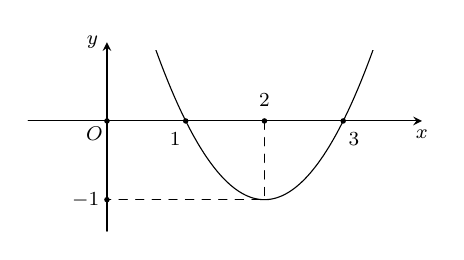
\begin{tikzpicture}[scale=1,>=stealth, font=\footnotesize, line join=round, line cap=round]
	\def\a{1} \def\b{-4} \def\c{3} % Hệ số
	\def\xmin{-1} \def\xmax{4}
	\def\ymin{-1.4} \def\ymax{1}	
	%\draw[color=gray!50,dashed] (\xmin,\ymin) grid (\xmax,\ymax);	
	\draw[->] (\xmin,0)--(\xmax,0) node [below]{$x$};
	\draw[->] (0,\ymin)--(0,\ymax) node [left]{$y$};
	\fill (0,0) circle (1pt) node[shift={(-135:2.5mm)}]{$O$};
	\clip (\xmin+0.1,\ymin+0.1) rectangle (\xmax-0.5,\ymax-0.1);
	\draw[smooth,samples=300] plot(\x,{\a*(\x)^2+\b*(\x)+\c});
	\foreach \s/\t in {1/-120,2/90,3/-60}%Trục Ox
	\fill (\s,0) circle (1pt) node[shift={(\t:3mm)}]{$\s$};
	\foreach \p/\r in {-1/180}%Trục Oy
	\fill (0,\p) circle (1pt) node[shift={(\r:3mm)}]{$\p$};
	\draw[dashed] (2,0)|-(0,-1);
\end{tikzpicture}
}
	\loigiai{
		Dựa vào đồ thị hàm số, $f(x) \ge 0$ khi và chỉ khi $x \le 1 $ hoặc $x \geq 3$.\\
		Tập nghiệm của bất phương trình là $(-\infty;1]\cup [3;+\infty)$.
	}
\end{bt}

% từ: cau-hoi/lop10/0D7_Bat_phuong_trinh_bac_2_mot_an/0D7-2-2_Giai_bat_phuong_trinh_bac_hai_biet_BXD_do_thi.tex
\begin{bt}%[0D7H2-2]%[Dự án đề kiểm tra GHKI NH22-23- Le Hung Thang]%[ma:277810e7]
	 Cho đồ thị của hàm số bậc hai $f(x)$. Tìm tập nghiệm của bất phương trình tương ứng.
\begin{listEX}[2]
	\item $f(x) \geq 0$\\
	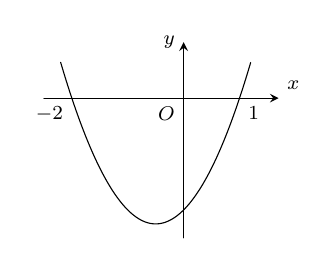
\begin{tikzpicture}[>=stealth,line join=round,line cap=round,font=\footnotesize,scale=0.71]
		\draw[->] (-2.5,0)--(1.7,0)node[above right]{$x$};
		\draw[->] (0,-2.5)--(0,1)node[left]{$y$};
		\fill (0,0)node[below left]{ $O$};
		\draw[black,samples=150,smooth,domain=-2.2:1.2] plot(\x,{(\x)^2+(\x)-2});
		\draw (-2,0)node[below left]{$-2$} (1,0)node[below right]{$1$};
	\end{tikzpicture}
	\item $f(x)<0$\\
	\begin{tikzpicture}[>=stealth,line join=round,line cap=round,font=\footnotesize,scale=0.71]
		\draw[->] (-.5,0)--(4,0)node[above right]{$x$};
		\draw[->] (0,-2.5)--(0,1)node[left]{$y$};
		\fill (0,0)node[below left]{ $O$};
		\draw[black,samples=150,smooth,domain=.45:3.5] plot(\x,{-1*(\x)^2+4*(\x)-4});
		\draw (2,0)node[above]{$2$}	;
	\end{tikzpicture}
\end{listEX}
\loigiai{
	\begin{enumerate}
	\item Dựa vào đồ thị $f(x) \geq 0\Leftrightarrow\hoac{&x\le -2\\&x\ge 1.}$\\
	Vậy tập nghiệm của bất phương trình là $S=(-\infty;-2]\cup[1;+\infty)$.
	\item Dựa vào đồ thị $f(x)<0\Leftrightarrow x\neq 2$.\\
	Vậy tập nghiệm của bất phương trình là $S=\mathbb{R}\setminus\{2\}$.
	\end{enumerate}
}
\end{bt}

% từ: cau-hoi/lop10/0D7_Bat_phuong_trinh_bac_2_mot_an/0D7-2-2_Giai_bat_phuong_trinh_bac_hai_biet_BXD_do_thi.tex
\begin{bt}%[0D7N2-2]%[Tex hóa SGK CD-CT,T7/22, Tuấn Nguyễn]%[ma:86d68f8e]
	Dựa vào đồ thị hàm số bậc hai $y=f(x)$ trong mỗi Hình $a), b), c)$, hãy viết tập nghiệm của mỗi bất phương trình sau: $f(x)>0; f(x)<0; f(x) \geq 0; f(x) \leq 0$.
	\begin{center}
		\begin{tikzpicture}[scale=0.5, font=\footnotesize, line join=round, line cap=round, >=stealth]
			\draw[->] (-1.5,0) -- (6,0)node[below] {$x$};
			\draw[->] (0,-2.5) -- (0,6)node[right] {$y$};
			\foreach \i in {-1,1,2,3,4}
			{	\draw (\i,-.05) -- (\i,.05);
				\draw (\i,0) node[below left]{$\i$};
			}
			\foreach \i in {-2,-1,1,2,3,4}
			{	\draw (-.05,\i) -- (.05,\i);
				\draw (0,\i) node[left]{$\i$};
			}
			\draw[samples=100,domain=-0.3:5.3]   plot (\x,{(\x)^2-5*(\x)+4});
			\node[below left] at (0,0) {$O$};
			\node[below] at (2.5,-2.7) {$a)$};
		\end{tikzpicture}
		\hspace*{.5cm}
		\begin{tikzpicture}[scale=0.5, font=\footnotesize, line join=round, line cap=round, >=stealth]
			\draw[->] (-1.5,0) -- (5,0)node[below] {$x$};
			\draw[->] (0,-2.5) -- (0,6)node[right] {$y$};
			\foreach \i in {-1,1,2,3,4}
			{	\draw (\i,-.05) -- (\i,.05);
				\draw (\i,0) node[below left]{$\i$};
			}
			\foreach \i in {-2,-1,1,2,3,4}
			{	\draw (-.05,\i) -- (.05,\i);
				\draw (0,\i) node[left]{$\i$};
			}
			\draw[samples=100,domain=-0.3:4.3]   plot (\x,{(\x)^2-4*(\x)+4});
			\node[below left] at (0,0) {$O$};
			\node[below] at (2.5,-2.7) {$b)$};
		\end{tikzpicture}
		\hspace*{.5cm}
		\begin{tikzpicture}[scale=0.5, font=\footnotesize, line join=round, line cap=round, >=stealth]
			\draw[->] (-1.5,0) -- (5,0)node[below] {$x$};
			\draw[->] (0,-2.5) -- (0,6)node[right] {$y$};
			\foreach \i in {-1,1,2,3,4}
			{	\draw (\i,-.05) -- (\i,.05);
				\draw (\i,0) node[below left]{$\i$};
			}
			\foreach \i in {-2,-1,1,2,3,4,5}
			{	\draw (-.05,\i) -- (.05,\i);
				\draw (0,\i) node[left]{$\i$};
			}
			\draw[samples=100,domain=-0.2:4.2]   plot (\x,{(\x)^2-4*(\x)+5});
			\node[below left] at (0,0) {$O$};
			\node[below] at (2.5,-2.7) {$c)$};
		\end{tikzpicture}
	\end{center}
	\loigiai{
		\begin{enumerate}
			\item Quan sát đồ thị Hình a), ta thấy
			\begin{itemize}
				\item $f(x)>0$ biểu diễn phần parabol $y=f(x)$ nằm phía trên trục hoành, tương ứng với $x<1$ hoặc $x>4$.\\
				Do đó tập nghiệm của bất phương trình $f(x)>0$ là $(-\infty; 1) \cup (4;+\infty)$ và tập nghiệm của bất phương trình $f(x) \geq 0$ là $(-\infty; 1] \cup [4;+\infty)$.
				\item $f(x)<0$ biểu diễn phần parabol $y=f(x)$ nằm phía dưới trục hoành, tương ứng với $1<x<4$.\\
				Do đó tập nghiệm của bất phương trình $f(x)<0$ là $(1; 4)$
				và tập nghiệm của bất phương trình $f(x) \leq 0$ là $[1; 4]$.
			\end{itemize}
			\item Quan sát đồ thị Hình b), ta thấy
			\begin{itemize}
				\item Tại $x=2$ thì $f(x)=0$.
				\item $f(x)>0$ biểu diễn phần parabol $y=f(x)$ nằm phía trên trục hoành, tương ứng với $x \neq 2$.
				Do đó tập nghiệm của bất phương trình $f(x)>0$ là $\mathbb{R} \setminus \{2\}$ và tập nghiệm của bất phương trình $f(x) \geq 0$ là $\mathbb{R}$.
				\item $f(x)<0$ biểu diễn phần parabol $y=f(x)$ nằm phía dưới trục hoành, mà phần đồ thị nằm phía trên trục hoành.\\
				Do đó bất phương trình $f(x)<0$ vô nghiệm và nghiệm của bất phương trình $f(x) \leq 0$ là $x=2$.
			\end{itemize}
			\item Quan sát đồ thị Hình c), ta thấy phần parabol nằm hoàn toàn phía trên trục hoành, do đó $f(x)>0$ với mọi $x \in \mathbb{R}$.\\
			Vậy tập nghiệm của bất phương trình $f(x)>0$ là $x \in \mathbb{R}$ và các bất phương trình $f(x)<0, f(x) \geq 0, f(x) \leq 0$ vô nghiệm.
		\end{enumerate}
	}
\end{bt}

% từ: cau-hoi/lop10/0D7_Bat_phuong_trinh_bac_2_mot_an/0D7-2-6_Bai_toan_co_tham_so.tex
\begin{bt}%[0D7V2-6]%[Dự án đề kiểm tra GKII NH22-23- Hieu Phan]%[THCS-THPT DIÊN HỒNG]%[ma:30644032]
Cho tam thức bậc hai $ f(x)=(m-1)x^2-(m-1)x+2m+1 $. Xác định $ m $ để $ f(x)\ge 0, \forall x \in \mathbb{R} $.
\loigiai{
    \begin{itemize}
        \item Xét $m=1$, khi đó $f(x)=3>0 \forall x \in \mathbb{R}$.
        \item Xét $m\ne 1$, khi đó \\
        $ f(x)\ge 0, \forall x \in \mathbb{R} $ khi và chỉ khi
        \begin{eqnarray*}
            \heva{&a>0 \\ & \Delta \le 0}&\Leftrightarrow& \heva{& m>1 \\ & (m-1)^2-4(m-1)(2m+1)\le 0 }\\
            &\Leftrightarrow& \heva{& m>1 \\ &-7m^2 +2m+5\le 0}\Leftrightarrow  \heva{& m>1 \\ &\hoac{& m\le -\dfrac{5}{7} \\ &  m\ge 1}}\Leftrightarrow m>1. 
        \end{eqnarray*}
    \end{itemize}
Vậy $m\ge 1$ thì $ f(x)\ge 0, \forall x \in \mathbb{R} $.
}
\end{bt}

% từ: cau-hoi/lop10/0D7_Bat_phuong_trinh_bac_2_mot_an/0D7-3-6_Toan_hinh_toan_thuc_te_ung_dung_phuong_trinh.tex
\begin{bt}%[0D7C3-6]%[ma:5ad70568]
	\immini{ 
	Một ngọn hải đăng được đặt tại vị trí $A$ cách bờ biển một khoảng $AB = 5$ km. Trên bờ biển có một cái  kho ở vị trí $C$ cách $B$ một khoảng $7$ km. Người canh hải đăng có thể chèo thuyền từ $A$ đến địa điểm $M$ trên bờ biển với vận tốc $4$ km/h, rồi đi bộ đến $C$ với vận tốc $6$ km/h. Người canh hải đăng tìm được cách đặt vị trí của $M$ để thời gian đến kho là $\dfrac{5\sqrt{5}+14}{12}$ (h). Khi đó vị trí điểm $M$ cách $B$ một khoảng bằng bao nhiêu km? (làm tròn đến hàng phần trăm).
	}{ 
	\begin{tikzpicture}[scale=.7,font=\footnotesize,line join=round,line cap=round,>=stealth]
			\path 
				(0,4) coordinate (A) 
				(0,0)  coordinate (B)
				(7,0)  coordinate (C)
				(3,0) coordinate (M); 
			\draw (A)--(B)--(C)--(A)--(M); 
			\draw[<->]  (-.5,0)--(-.5,4) node[midway,left]{$5$ km};
			\draw[<->] (0,-.7)--(7,-.7)  node[midway,below]{$7$ km};
			 \foreach \x/\g in{A/90,B/-120,C/0,M/60}
			 \fill[black](\x) circle (1pt)
				($(\x)+(\g:4mm)$)  node{$\x$};
			\draw pic[draw,angle radius=2mm] {right angle  = A--B--C};
		\end{tikzpicture}
	 }
	 \shortans{4,47}
	\loigiai{ 
	\immini{ 
	Đặt $BM=x$ (km), với $0\le x\le 7$. Suy ra $CM =  7-x$ (km). \\
	 Suy ra $AM=\sqrt{25+x^2}$ (km).\\
	Thời gian chèo  thuyền trên đoạn đường biển $AM$ là
	$$t_1 = \dfrac{\sqrt{25  + x^2}}{4}\;(\text{h})$$
	Thời gian  đi bộ trên đoạn đường $CM$ là
	$$t_2 = \dfrac{7-x}{6}\;(\text{h})$$ 
	 }{
	\begin{tikzpicture}[scale=.8,font=\footnotesize,line join=round,line cap=round,>=stealth]
			 \path
				(0,4) coordinate  (A)
				(0,0) coordinate (B) 
				 (7,0) coordinate (C)
				 (3,0) coordinate (M);
			 \draw (A)--(B)--(C)--(A)--(M);
			\draw[<->] (-.5,0)--(-.5,4) node[midway,left]{$5$  km};
			\draw[<->] (0,-.7)--(3,-.7)  node[midway,below]{$x$ km};
			\draw[<->]  (3,-1)--(7,-1) node[midway,below]{$7-x$ km};
			 \foreach \x/\g in{A/90,B/-120,C/0,M/60}
			 \fill[black](\x) circle (1pt)
				($(\x)+(\g:4mm)$) node{$\x$}; 
			\draw pic[draw,angle radius=2mm] {right angle  = A--B--C};
		\end{tikzpicture}
	 }
	\noindent Vì  tổng thời gian đi từ $A$ đến $C$ hết $\dfrac{5\sqrt{5}+14}{12}$ (h) nên ta có phương trình
	\begin{eqnarray*}
		&&\dfrac{\sqrt{25+x^2}}{4}+\dfrac{7-x}{6}=  \dfrac{5\sqrt{5}+14}{12} \\
		&\Leftrightarrow &2x+5\sqrt{5}=3\sqrt{x^2+25}\\ &\Leftrightarrow &5x^2-20\sqrt{5}x+100=0\\ &\Leftrightarrow &x=2\sqrt{5}. 
	\end{eqnarray*}
	Vậy vị trí điểm $M$ cách $B$ một khoảng  bằng $2\sqrt{5}\approx 4{,}47$ km.
	} 
\end{bt}

% từ: cau-hoi/lop10/0D7_Bat_phuong_trinh_bac_2_mot_an/0D7-3-6_Toan_hinh_toan_thuc_te_ung_dung_phuong_trinh.tex
\begin{bt}%[0D7C3-6]%[ma:eda4a6ee]
	Cho tam giác $ABC$ vuông tại $A$ có $BC=6$ cm. Điểm $D$ nằm trên tia $AB$ sao cho $DB=3$ cm, $DC=8$ cm (xem hình vẽ). Đặt $AC=x$. Tính diện tích tam  giác $BCD$.
	\begin{center}
		\begin{tikzpicture}
				 \def\r{5}
				\path  (0:0) coordinate (A)
					++(0:\r)  coordinate (C)
					(A)++(-90:0.9*\r)  coordinate (D)
					(A)++(-90:0.45*\r)  coordinate (B);
				\draw (A)--(C) node [midway,above]  {$x$}
					(C)--(D)  node [midway,below right] {$8$ cm}
					(D)--(B) node [midway,left]  {$3$ cm}
					(B)--(A) 
					pic[draw,angle radius=2mm]{right angle=D--A--C} 
					(B)--(C) node [midway,above left] {$6$ cm}; 
				\foreach \x/ \goc  in {A/135,D/-135,C/45,B/180}
				\fill  (\x) circle (1pt)
					($(\x)+(\goc:3mm)$) node  {$\x$};
			\end{tikzpicture}
	\end{center}
	 \loigiai{
		Áp dụng định lí Py-ta-go cho tam giác $ABC$  vuông tại $A$, ta được $AC^2+AB^2=BC^2$.\\
		 Suy ra $AB=\sqrt{BC^2-AC^2}=\sqrt{6^2-x^2}=\sqrt{36-x^2}$ (cm).\\
		Áp dụng định lí Py-ta-go cho tam  giác $ACD$ vuông tại $A$, ta được $AC^2+AD^2=CD^2$.\\
		Suy ra $AD=\sqrt{CD^2-AC^2}=\sqrt{8^2-x^2}=\sqrt{64-x^2}$  (cm).\\
		 Mà $AB+BD=AD$ nên $\sqrt{36-x^2}+3=\sqrt{64-x^2}$.
		Bình phương hai  vế của phương trình, ta được
		$$36-x^2+6\sqrt{36-x^2}+9=64-x^2\Rightarrow  \sqrt{36-x^2}=\dfrac{19}{6} \Rightarrow x^2=\dfrac{935}{36} \Rightarrow x =\dfrac{\sqrt{935}}{6}\approx 5{,}1.$$
		Thử lại, ta  thấy $x=\dfrac{\sqrt{935}}{6}$ thỏa mãn phương trình ban đầu.\\
		Vậy diện tích của tam giác $BCD$ là  $\dfrac{1}{2} \cdot 5{,}1\cdot 3\approx7{,}65$ (cm$^2$).
	 }
\end{bt}

% từ: cau-hoi/lop10/0D7_Bat_phuong_trinh_bac_2_mot_an/0D7-3-6_Toan_hinh_toan_thuc_te_ung_dung_phuong_trinh.tex
\begin{bt}%[0D7V3-6]%[ma:f32581bf]
	Người ta làm ra một cái thang bắc lên tầng hai của một ngôi nhà (hình vẽ), muốn vậy họ cần làm một thanh đỡ $BC$ có chiều dài $4\,\mathrm{m}$, đồng thời muốn đảm bảo kỹ thuật thì tỉ số độ dài $\dfrac{CE}{BD}=\dfrac{5}{3}$. Hỏi vị trí $A$ cách vị trí $B$ bao nhiêu mét?
	\begin{center}\begin{tikzpicture}[scale=1.5, font=\footnotesize, line join=round, line cap=round,>=stealth]
		\path 
		(-0.8,-1) coordinate (A)
		(4,-1) coordinate (D) 
		(0,-1) coordinate (A') 
		(4,0.3) coordinate (E)
		(4,3) coordinate (X)
		($(A)!3/5!(D)$)coordinate(B)
		($(A)!3/5!(E)$)coordinate(C)
		;
		\draw (X)--(6,3)--(6,-1)--(4,-1)--(X) (-1.5,-1)--(6.6,-1) (B)--(C) (A)--(E);
		\draw[fill=cyan] (X)--(6,3)--(6,-1)--(4,-1)--(X);
		\foreach \i in {2,3,4,5}
		\draw[fill=white] ({4+1/3},{-1+(2/3)*(\i-1)})--({4+1/3},{-1+(2/3)*(\i-1)+0.5})--({4+2/3},{-1+(2/3)*(\i-1)+0.5})--({4+2/3},{-1+(2/3)*(\i-1)})--cycle 
		({5+1/3},{-1+(2/3)*(\i-1)})--({5+1/3},{-1+(2/3)*(\i-1)+0.5})--({5+2/3},{-1+(2/3)*(\i-1)+0.5})--({5+2/3},{-1+(2/3)*(\i-1)})--cycle;
		\foreach \x/\g in {A/-90,D/-90,B/-90,C/90,E/140} 
		\fill[black] (\x) circle (1pt)+(\g:3mm) node {$\x$};
		\draw ($(B)!1/2!(C)$)node[right]{$4\,\mathrm{m}$};
		\end{tikzpicture}\end{center}	
	\shortans[oly]{3}
	\loigiai
	{
		Đặt $AB=x>0$. Xét tam giác $ABC$ vuông tại $B$ có $AC=\sqrt{x^2+4}$.\\
		Theo tính chất định lí Ta-let, ta có 
		$$\dfrac{AC}{AB}=\dfrac{CE}{BD}\Rightarrow \dfrac{\sqrt{x^2+16}}{x}=\dfrac{5}{3}\Rightarrow \dfrac{x^2+16}{x^2}=\dfrac{25}{9}\Rightarrow x=3.$$
		Vậy vị trí $B$ cách $A$ một khoảng là $3\,\mathrm{m}$.
		}
\end{bt}

% từ: cau-hoi/lop10/0D8_Dai_so_to_hop/0D8-2-6_Bai_toan_co_yeu_to_hinh_hoc.tex
\begin{ex}%[0D8N2-6]%[ma:9ce00d02]
	Trong mặt phẳng cho tập hợp gồm $25$ điểm phân biệt. Có bao nhiêu véc-tơ khác véc-tơ $\overrightarrow{0}$ có điểm đầu và điểm cuối thuộc  tập hợp điểm này?
	\choice 
		 {$50$}
		 {$300$}
		{\True $600$} 
		{$625$} 
	 \loigiai{
		Số véc-tơ khác $\overrightarrow{0}$ có điểm đầu và điểm cuối được tạo ra bởi $25$ điểm phân  biệt là $\mathrm{A}_{25}^2=600$ véc-tơ.
	 }
\end{ex}

% từ: cau-hoi/lop10/0D8_Dai_so_to_hop/0D8-2-6_Bai_toan_co_yeu_to_hinh_hoc.tex
\begin{bt}%[0D8H2-6]  Tìm số giao điểm tối đa của%[ma:550855f6]
	\begin{enumerate}
		\item $10$ đường thẳng phân biệt. 
		\item $6$ đường tròn phân biệt.
	\end{enumerate}
	\loigiai{
		\begin{enumerate}
			\item Cứ hai đường thẳng phân biệt thì có tối đa ${1}$ giao điểm, nên số giao điểm chính là số cách chọn ${2}$ đường thẳng bất kỳ trong ${10}$ đường thẳng phân biệt. Vậy số giao điểm tối đa của ${10}$ đường thẳng phân biệt là $\mathrm{C}{10}^{2}=45$. 
			\item Hai đường tròn phân biệt có tối đa ${2}$ giao điểm $\Rightarrow$ Số giao điểm tối đa của ${6}$ đường tròn phân biệt là ${2\cdot C_{6}^{2}=30}$ điểm.
		\end{enumerate}
	}
\end{bt}

% từ: cau-hoi/lop10/0D8_Dai_so_to_hop/0D8-3-3_Tim_he_so_so_hang_trong_khai_trien_bang_tam_g.tex
\begin{ex}%[0D8H3-3]%[ma:8e4a8223]
	Biết $\left(1+\sqrt[3]2\right)^4=a_0+a_1  \sqrt[3]2+a_2 \sqrt[3]4$. Tính $a_1a_2$.
	\choice 
		{$a_1 a_2=24$} 
		{$a_1  a_2=8$}
		{$a_1 a_2=54$} 
		 {$a_1 a_2=36$}
	\loigiai{ 
		Ta  có
		 \allowdisplaybreaks
		\begin{align*}
			\left(1+\sqrt[3]{2}\right)^4&=1^4+4\cdot  1^3\left(\sqrt[3]{2}\right)^1+6\cdot 1^2\left(\sqrt[3]{2}\right)^2+4\cdot 1^1\left(\sqrt[3]{2}\right)^3+\left(\sqrt[3]{2}\right)^4
			 \\
			&=1+4 \sqrt[3]{2}+6  \sqrt[3]{4}+8+2 \sqrt[3]{2} \\
			&=9+6 \sqrt[3]{2}+6 \sqrt[3]{4}. 
		\end{align*}
		 Suy ra $a_1\cdot a_2=6\cdot 6=36$.
	} 
\end{ex}

% từ: cau-hoi/lop10/0H4_He_thuc_luong_trong_tam_giac/0H4-3-1_Giai_tam_giac.tex
\begin{ex}%[0H4H3-1]%[ma:8dd06fb9]
	Cho tam giác  $ABC$, biết bán kính đường tròn ngoại tiếp tam giác là $R=15$, diện tích tam giác $ABC$ bằng $45$ và $\widehat{A}=30^\circ$. Tính khoảng cách từ đỉnh $A$ đến cạnh $BC$.
	 \choice {\True $15$}{$20$}{$6$}{$\dfrac{19}{2}$}
	 \loigiai{
		Gọi $d$ là khoảng cách từ đỉnh $A$ đến  cạnh $BC$.\\
		Áp dụng định  lý sinta có $a=2R\sin A=2\cdot 15\cdot\sin30^\circ=15$.\\
		 Mặt khác $S_{ABC}=\dfrac{1}{2}ad$.\\
		Suy ra  $d=\dfrac{2S_{ABC}}{a}=\dfrac{2\cdot45}{15}=6$.\\
		Vậy khoảng cách từ đỉnh $A$ đến cạnh $BC$  là $d=6$.
	 }
\end{ex}

% từ: cau-hoi/lop10/0H4_He_thuc_luong_trong_tam_giac/0H4-3-1_Giai_tam_giac.tex
\begin{bt}%[0H4N3-1]%[Tex hóa SGK CD-CT,T7/22, Phạm Tiến Long]%[ma:2b2b2071]
	Cho tam giác $ABC$, biết cạnh $a=75$ cm, $\widehat{B}=80^\circ$, $\widehat{C}=40^\circ$.
	\begin{enumerate}[a)]
		\item Tính các cạnh, các góc còn lại của tam giác $ABC$.
		\item Tính bán kính đường tròn ngoại tiếp của tam giác $ABC$.
	\end{enumerate}
	\loigiai{
		\begin{enumerate}[a)]
			\item Ta có $a=75$ cm; $\widehat{A}=180^\circ-\left(80^\circ+40^\circ\right)=60^\circ$.\\
			Áp dụng định lí sin, ta có $\dfrac{a}{\sin A}=\dfrac{b}{\sin B}=\dfrac{c}{\sin C}=2R$.\\
			Suy ra 
			\begin{eqnarray*}
				b&=&\dfrac{a\sin B}{\sin A}=\dfrac{75 \cdot \sin 80^\circ}{\sin 60^\circ} \approx 85{,}29\text{ cm};\\
				c&=&\dfrac{a\sin C}{\sin A}=\dfrac{75 \cdot \sin 40^\circ}{\sin 60^\circ} \approx 55{,}67\text{ cm}.
			\end{eqnarray*}
			\item $R=\dfrac{a}{2 \cdot \sin A}=\dfrac{75}{2\sin 60^\circ}=25\sqrt{3}$ cm.
		\end{enumerate}
	}
\end{bt}

% từ: cau-hoi/lop10/0H5_Vecto_chua_xet_toa_do/0H5-4-3_Dang_thuc_ve_tich_vo_huong_hoac_do_dai.tex
\begin{bt}%[0H5V4-3]%[ma:50b3d0d4]
	
	Chứng minh rằng tổng bình phương hai đường chéo của hình bình hành bằng tổng bình phương bốn cạnh của nó.
	\loigiai{
		\begin{center}
			\begin{tikzpicture}[scale=0.9,font=\footnotesize,line join=round,line cap=round,>=stealth]	
				\def\d{4}
				\def\r{3}
				\path (0:0) coordinate (B)
				++(0:\d) coordinate (C)
				++(50:\r) coordinate (D)
				($(B)+(D)-(C)$) coordinate (A)
				($(A)!0.5!(C)$) coordinate (O);
				\draw (A)--(B)--(C)--(D)--cycle (A)--(C) (B)--(D);
				\foreach \x/ \goc in {A/180,B/180,C/0,D/0,O/90} 
				\fill (\x) circle (1pt)	
				($(\x)+(\goc:3mm)$) node {$\x$};
			\end{tikzpicture}
		\end{center}
		Xét hình bình hành $ABCD$. Gọi $O$ là giao điểm của $AC$ và $BD$ thì $AO$ là trung tuyến của tam giác $ABD$.\\
		Ta có\\
		$AO^2=\dfrac{AB^2+AD^2}{2}-\dfrac{BD^2}{4}\Leftrightarrow \dfrac{AC^2}{4}=\dfrac{AB^2+AD^2}{2}-\dfrac{BD^2}{4}$ $\Leftrightarrow AC^2+BD^2=2\left( AB^2+AD^2 \right)$.}
\end{bt}

% từ: cau-hoi/lop10/0H9_Phuong_phap_toa_do_trong_mat_phang/0H9-2-3_Dang_thuc_ve_tich_vo_huong_hoac_do_dai.tex
\begin{ex}%[0H9V2-3]%[ma:ff5c03ca]
	Trong hệ tọa độ $Oxy$, cho các điểm $A(0;3)$, $B(4;3)$, $C(2;0)$. Gọi $I$  là trung điểm của đoạn $OA$, $M(x;y)$ là một điểm tùy ý. Các khẳng định sau đây đúng hay sai?
	\choiceTF 
		 {$\overrightarrow{OI}\cdot\overrightarrow{IB}+\overrightarrow{AI}\cdot\overrightarrow{IB}\neq 0$}
		 {\True $AB^2+\overrightarrow{AB}\cdot\overrightarrow{BC}+\overrightarrow{AB}\cdot\overrightarrow{CA}=0$}
		 {$(\overrightarrow{IA}+\overrightarrow{IB})\cdot\overrightarrow{IO}=\dfrac{9}{2}$}
		{\True $\overrightarrow{MA}\cdot\overrightarrow{BC}+\overrightarrow{MB}\cdot\overrightarrow{CA}+\overrightarrow{MC}\cdot\overrightarrow{AB}=0$} 
	\loigiai{ 
		\begin{itemchoice}
			 \itemch Ta có $\overrightarrow{OI}\cdot\overrightarrow{IB}+\overrightarrow{AI}\cdot\overrightarrow{IB}=\overrightarrow{IB}\cdot(\overrightarrow{OI}+\overrightarrow{AI})=\overrightarrow{IB}\cdot\overrightarrow{0}=0$.
			\itemch Ta có $AB^2+\overrightarrow{AB}\cdot\overrightarrow{BC}+\overrightarrow{AB}\cdot\overrightarrow{CA}=\overrightarrow{AB}\cdot  (\overrightarrow{AB}+\overrightarrow{BC}\cdot\overrightarrow{CA})=\overrightarrow{AB}\cdot\overrightarrow{0}=0$.
			\itemch Do $I$ là trung điểm  của đoạn $OA$ nên $I\left(0;\dfrac{3}{2}\right)$.\\
			Ta có $\overrightarrow{IA}=\left(0;\dfrac{3}{2}\right)$,  $\overrightarrow{IB}=\left(4;\dfrac{3}{2}\right)$ và $\overrightarrow{IO}=\left(0;-\dfrac{3}{2}\right)$.\\
			Do đó $\overrightarrow{IA}+\overrightarrow{IB}=(4;3)$, suy  ra $(\overrightarrow{IA}+\overrightarrow{IB})\cdot\overrightarrow{IO}=-\dfrac{9}{2}$.
			\itemch Ta  có $\overrightarrow{MA}=(-x;3-y)$, $\overrightarrow{BC}=(-2;-3)$.\\
			Suy  ra $\overrightarrow{MA}\cdot\overrightarrow{BC}=2x+3y-9$.\\
			Tương tự  $\overrightarrow{MB}\cdot\overrightarrow{CA}=2x-3y+1$, $\overrightarrow{MC}\cdot\overrightarrow{AB}=-4x+8$.\\
			Vậy $\overrightarrow{MA}\cdot\overrightarrow{BC}+\overrightarrow{MB}\cdot\overrightarrow{CA}+\overrightarrow{MC}\cdot\overrightarrow{AB}=0$ 
		\end{itemchoice}
	 }
\end{ex}

% từ: cau-hoi/lop10/0H9_Phuong_phap_toa_do_trong_mat_phang/0H9-3-2_Phuong_trinh_duong_thang.tex
\begin{bt}%[0H9H3-2]%[ma:376a1a90]
	Trong mặt phẳng toạ độ $Oxy$, cho tam giác $MNP$ có $M(2 ; 1), N(-1 ; 3), P(4 ; 2)$.
	\begin{enumerate}[a)]
	\item Tìm toạ độ của các vectơ $\overrightarrow{O M}, \overrightarrow{M N}, \overrightarrow{M P}$;
	\item Tính tích vô hưởng $\overrightarrow{MN}.\overrightarrow{M P}$;
	\item Tính độ dài các đoạn thẳng $M N, M P$;
	\item Tính $\cos \widehat{N M P}$;
	\item Tìm tọa độ trung điểm $I$ của $N P$ và trọng tâm $G$ của tam giác $M N P$.
	\end{enumerate}
\loigiai{
	\begin{enumerate}[a)]
		\item $\overrightarrow{O M}= (2;1).$\\
		$\overrightarrow{MN}= (-3;2).$\\
		$\overrightarrow{MP}= (2;1).$
		\item Tích vô hướng $\overrightarrow{MN}.\overrightarrow{MP}=-3.2+2.1=-4.$
		\item Độ dài đoạn thẳng $MN=\sqrt{(-3)^2+2^2}=\sqrt{13}.$\\
		Độ dài đoạn thẳng $MP=\sqrt{2^2+1^2}=\sqrt{5}.$
		\item $\cos \widehat{NMP}=\dfrac{\overrightarrow{MN}.\overrightarrow{MP}}{\left| \overrightarrow{MN}\right| .\left| \overrightarrow{MP}\right| }=\dfrac{-4}{\sqrt{13}.\sqrt{5}}=\dfrac{-4\sqrt{65}}{65}.$
		\item Tọa độ trung điểm $I$ của $NP$ là \\
		$N\left( \dfrac{x_N+x_P}{2};\dfrac{y_N+y_P}{2}\right) =N\left( \dfrac{-1+4}{2};\dfrac{3+2}{2}\right)=N\left( \dfrac{3}{2};\dfrac{5}{2}\right)$.\\
		Trọng tâm $G$ của tam giác $MNP$ là \\
		$G\left( \dfrac{x_M+x_N+x_P}{3};\dfrac{y_M+y_N+y_P}{3}\right) =G\left( \dfrac{2-1+4}{3};\dfrac{1+3+2}{3}\right)=G\left( \dfrac{5}{3};2\right)$.
		\end{enumerate}
}
\end{bt}

% từ: cau-hoi/lop10/0H9_Phuong_phap_toa_do_trong_mat_phang/0H9-3-6_Bai_toan_tim_diem.tex
\begin{bt}%[0H9C3-6]%[ma:41a9e5a0]
	Trong mặt phẳng $Oxy$ cho ngũ giác $ABCDE$ với $A(6;0), B(2;4),
	C(-2;4), D(-4;0)$ và $E(0;-6)$ (tham khảo hình vẽ). Tìm số giá trị nguyên của $m$ sao cho điểm $M(m;m+4)$ nằm trên hình ngũ giác $ABCDE$ tính cả năm cạnh $AB, BC,
	CD, DE, EA$.
\begin{center}
	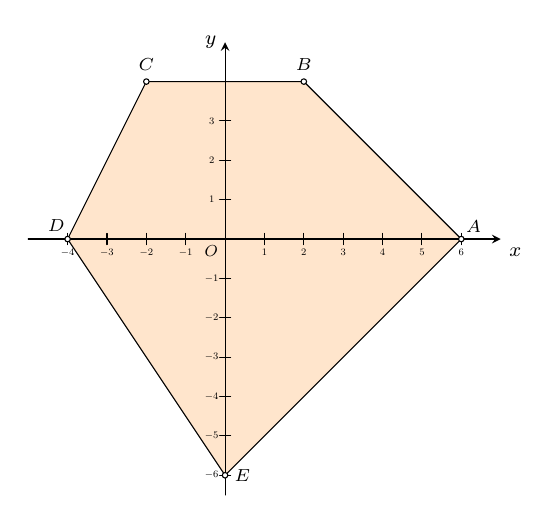
\begin{tikzpicture}[>=stealth,line join=round,line cap=round,font=\footnotesize,scale=1,x=0.5cm,y=0.5cm]		
		\path (6,0) coordinate (A)
		(2,4) coordinate (B)
		(-2,4) coordinate (C)
		(-4,0) coordinate (D)
		(0,-6) coordinate (E);		
		\fill[orange!20] (A)--(B)--(C)--(D)--(E)--cycle;
		\draw[->] (-5,0)--(7,0) node[below right] {$x$};
		\draw[->] (0,-6.5)--(0,5) node[left] {$y$};
		\draw (0,0) node[below left,scale=0.8] {$O$};
		\draw (A)--(B)--(C)--(D)--(E)--cycle;
		\foreach \x/\g in {-4/-90,-3/-90,-2/-90,-1/-90,1/-90,2/-90,3/-90,4/-90,5/-90,6/-90}
		\draw[thin] (\x,2pt)--(\x,-2pt) + (\g:1mm) node [scale=0.5] {$\x$};
		%Vẽ các điểm trên trục Oy
		\foreach \y/\g in {-6/180,-5/180,-4/180,-3/180,-2/180,-1/180,1/180,2/180,3/180}
		\draw[thin] (2pt,\y)--(-2pt,\y) + (\g:1mm) node [scale=0.5] {$\y$};
		\foreach \t/\g in {A/45,B/90,C/90,D/130,E/0}{
			\draw[fill=white] (\t) circle (1pt) node[shift={(\g:7pt)},font=\scriptsize]{$ \t $};
		}
	\end{tikzpicture}
\end{center}
	\loigiai{
		\begin{itemize}
			\item  Nhận thấy hình ngũ giác $ABCDE$ tính cả $5$ cạnh của nó là miền nghiệm của hệ bất phương trình gồm $5$ bất phương trình có miền nghiệm là nửa mặt phẳng chứa điểm $O(0;0)$ và lần lượt có các bờ là các đường $AB, BC, CD, DE, EA$.
		\item Phương trình đường thẳng $AB \colon x+y-6=0$. Bất phương trình có miền nghiệm là nửa mặt phẳng bờ $AB$ (tính cả bờ $AB$) và chứa điểm $O(0;0)$ là $x+y\le 6$.
		\item Phương trình đường thẳng $BC \colon y=4$. Bất phương trình có miền nghiệm là nửa mặt phẳng bờ $BC$ (tính cả bờ $BC$) và chứa điểm $O(0;0)$ là $y\le 4$.
		\item Phương trình đường thẳng $ CD \colon 2x-y+8=0$. Bất phương trình có miền nghiệm là nửa mặt phẳng bờ $CD$ (tính cả bờ $CD $) và chứa điểm $O(0;0)$ là $2x-y+8\ge 0$.
		\item Phương trình đường thẳng $DE \colon 3x+2y+12=0$. Bất phương trình có miền nghiệm là nửa mặt phẳng bờ $DE$ (tính cả bờ $DE$ và chứa điểm $O(0;0)$ là $3x+2y+12\ge 0$.
		\item Phương trình đường thẳng $EA \colon x-y-6=0$. Bất phương trình có miền nghiệm là nửa mặt phẳng bờ $EA$ (tính cả bờ Phương trình đường thẳng: $x-y-6=0$. Bất phương trình có miền nghiệm là nửa mặt phẳng bờ $EA$ (tính cả bờ $EA$ và chứa điểm $O(0;0)$ là $x-y-6\le 0$ và chứa điểm $O(0;0)$ là $x-y-6\le 0$.
		\item Như vậy hình ngũ giác $ABCDE$ tính cả $5$ cạnh của nó là miền nghiệm của hệ bất phương trình.
		\[\left\{\begin{array}{l}
			{x+y-6\le 0} \\
			{y\le 4} \\
			{2x-y+8\ge 0} \\
			{3x+2y+12\ge 0} \\
			{x-y-6\le 0.} 
		\end{array}\right. (*)\] 
		\item Điểm $M\ (m;m+4)$ nằm trên hình ngũ giác $ABCDE$ tính cả năm cạnh của nó khi và chỉ khi $M\ (m;m+4)$ là một nghiệm của hệ $(*)$ tức là \[\left\{\begin{array}{l}
			{m+m+4-6\le 0} \\
			{m+4-4\le 0} \\
			{2m-m-4+8\ge 0} \\
			{3m+2m+20\ge 0} \\
			{m-m-4-6\le 0} 
		\end{array}\right. 
		\Leftrightarrow \left\{\begin{array}{l}
			{m\le 1} \\
			{m\le 0} \\
			{-4\le m} 
		\end{array}\right. 
		\Leftrightarrow-4\le m\le 0.\] 
		Do $m$ nguyên nên $m\in \left\{-4,-3,-2,-1{,}0\right\}$.
	\end{itemize}
		Vậy có 5 giá trị nguyên của $m$ thoả mãn yêu cầu bài toán.
	}
\end{bt}

% từ: cau-hoi/lop11/1D1_Ham_so_luong_giac_va_phuong_trinh_luong/1D1-1-1_Cau_hoi_ly_thuyet.tex
\begin{ex}%[1D1N1-1]%[ma:0d6b1b1a]
	Trong các mệnh đề sau, mệnh đề nào  đúng ?
	\choice 
		{Các hàm số $y=\sin x$, $ y=\cos x$, $y=\cot x$  đều là hàm số chẵn}
		{\True Các hàm số $y=\sin x$, $y=\cot x$, $y=\tan  x$ đều là hàm số lẻ}
		 {Các hàm số $y=\sin x$, $y=\cos x$, $y=\tan x$ đều là hàm số chẵn}
		{Các hàm số $y=\sin x$, $y=\cos x$, $y=\cot x$ đều là hàm số lẻ} 
	\loigiai{ 
		 Hàm số $y=\sin x$, $y=\tan x$, $y=\cot x$ là hàm số lẻ.\\
	Hàm số $y=\cos x$ là hàm số  chẵn. }
\end{ex}

% từ: cau-hoi/lop11/1D1_Ham_so_luong_giac_va_phuong_trinh_luong/1D1-1-2_Chuyen_doi_don_vi_do_va_radian.tex
\begin{ex}%[1D1B1-2]%[ma:481837d4]
	Hãy chọn khẳng định \textbf{sai} trong các khẳng định dưới đây: Trong  khoảng $\left(\dfrac{\pi}{2};\pi\right)$ thì
	\choice 
		{\True hàm số $y=\cot x$ là hàm số đồng biến} 
		{hàm số $y=\tan x$ là hàm số  đồng biến}
		{hàm số $y=\cos x$ là hàm  số nghịch biến}
		{hàm số  $y=\sin x$ là hàm số nghịch biến}
	\loigiai{ 
		Trong khoảng $\left(\dfrac{\pi}{2};\pi\right)$ thì hàm số  $y=\cot x$ là hàm số nghịch biến.
	 }
\end{ex}

% từ: cau-hoi/lop11/1D1_Ham_so_luong_giac_va_phuong_trinh_luong/1D1-1-4_Do_dai_cua_mot_cung_tron.tex
\begin{ex}%[1D1N1-4]%[ma:9aafea7b]
	Cho $\pi <\alpha  <\dfrac{3\pi}{2}$, tìm phát biểu đúng trong các phát biểu sau.
	\choice 
		 {$\sin x>0$}
		{$\cos  x>0$}
		{\True $\tan  x>0$}
		{$\cot x<0$} 
	 \loigiai{
	Ta có $\pi <\alpha <\dfrac{3\pi}{2}\Rightarrow \heva{&\sin x<0 \\&\cos x<0 \\&\tan x>0  \\&\cot x>0 .}$}
\end{ex}

% từ: cau-hoi/lop11/1D1_Ham_so_luong_giac_va_phuong_trinh_luong/1D1-2-1_Cau_hoi_ly_thuyet.tex
\begin{ex}%[1D1N2-1]%[ma:43374932]
	\immini 
	{Cho góc lượng giác có số đo bằng $\dfrac{-3\pi}{4}$. Điểm nào sau đây  là điểm biểu diễn góc lượng giác đã cho trên đường tròn lượng giác?
	\choice 
		{Điểm  $A$}
		{Điểm  $B$}
		{\True Điểm  $C$}
		 {Điêm $D$}}
		{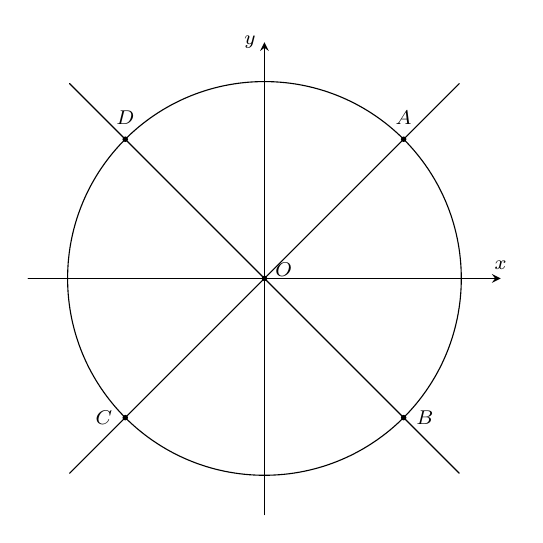
\begin{tikzpicture}[line join=round,line cap=round,>=stealth,font=\footnotesize,scale=1]
		\def\r{2.5} 
		\draw[-stealth]  (-3,0)--(3,0) node[above]{$x$};
		 \draw[-stealth] (0,-3)--(0,3) node[left]{$y$};
		\draw (45:\r+1)--(225:\r+1)  node[above]{};
		\draw (135:\r+1)--(315:\r+1)  node[left]{};
		 \path
			(0,0) coordinate (O) 
			 (45:\r) coordinate (A)
			(135:\r)  coordinate (D)
			 (225:\r) coordinate (C)
			 (315:\r) coordinate (B);
		\draw (O) circle (\r); 
		\foreach \p/\r  in {O/25,A/90,B/0,D/90,C/180}
		\fill (\p)  circle (1pt) node[shift={(\r:3mm)}]{$\p$};
	\end{tikzpicture}
		 }
	 \loigiai{
		Điểm $C$ nằm ở vị  trí $-135^\circ=-\dfrac{3\pi}{4}$.
	} 
\end{ex}

% từ: cau-hoi/lop11/1D1_Ham_so_luong_giac_va_phuong_trinh_luong/1D1-2-1_Cau_hoi_ly_thuyet.tex
\begin{ex}%[1D1Y2-1]%[ma:173efa7c]
	Phương trình $\cos x  =\dfrac{\sqrt{3}}{2}$ có nghiệm là
	 \choice
		{$x=  \dfrac{\pi}{6}+k\pi$}
		{$\hoac {&x=\dfrac{\pi}{6}+k\pi \\& x=\dfrac{5\pi}{6}+k\pi}$} 
		 {$\hoac {&x=\dfrac{\pi}{6}+k2\pi \\& x=\dfrac{5\pi}{6}+k2\pi}$}
		 {\True $x= \pm \dfrac{\pi}{6}+k2\pi $}
	\loigiai{ Phương trình $\cos x =\dfrac{\sqrt{3}}{2} \Leftrightarrow \cos  x =\cos \left( \dfrac{\pi}{6}\right)\Leftrightarrow x= \pm \dfrac{\pi}{6}+k2\pi, k\in \mathbb{Z}. $
	} 
\end{ex}

% từ: cau-hoi/lop11/1D1_Ham_so_luong_giac_va_phuong_trinh_luong/1D1-2-2_Xet_dau_gia_tri_luong_giac_Tinh_gia_tri_luong.tex
\begin{ex}%[1D1N2-2]%[ma:86e92a6c]
	\immini[thm]{Cho góc hình học $uOv=30^\circ$. Xác  định số đo của góc lượng giác $(Ou,Ov)$.
	 \choice
		{  $\mathrm{\text{sđ}}(Ou,Ov)=-30^\circ+k360^\circ$, $k \in \mathbb{Z}$}
		 {\True $\mathrm{\text{sđ}}(Ou,Ov)=30^\circ+k360^\circ$, $k \in \mathbb{Z}$}
		{$\mathrm{\text{sđ}}(Ou,Ov)=150^\circ+k360^\circ$, $k \in \mathbb{Z}$} 
		{$\mathrm{\text{sđ}}(Ou,Ov)=-150^\circ+k360^\circ$, $k \in \mathbb{Z}$}}{\begin{tikzpicture}
		\draw (0,0)--(5,0); 
		\draw (0,0)--(30:4); 
		\draw  (5,0) node[below]{$u$}
			 (0,0) node[left]{$O$};
		 \draw (30:4) node[left]{$v$};
		 \draw (5,0) coordinate (A)--(0:0) coordinate (B)--(30:4) coordinate (C)
			pic [draw,->]{angle=A--B--C}; 
	\end{tikzpicture}
		} 
	\loigiai{ 
		Các góc lượng  giác tia đầu $Ou$, tia cuối $Ov$ có số đo là $\mathrm{\text{sđ}}(Ou,Ov)=30^\circ+k360^\circ$, $k \in \mathbb{Z}$.
	} 
\end{ex}

% từ: cau-hoi/lop11/1D1_Ham_so_luong_giac_va_phuong_trinh_luong/1D1-2-2_Xet_dau_gia_tri_luong_giac_Tinh_gia_tri_luong.tex
\begin{ex}%[1D1V2-2]%[ma:4609ab3c]
	Biểu thức $A=\sin^210^\circ+\sin^220^\circ+\cdots +\sin^2180^\circ  $ có giá trị bằng
	 \choice
		 {$A=6$}
		 {$A=8$}
		{$A=3$} 
		{\True  $A=9$}
	\loigiai{ Ta có $\sin\left(90^\circ+\alpha\right)=\cos\alpha  $.\\
	Suy ra  $\sin 100^\circ=\cos 10^\circ\Rightarrow{\sin^2}100^\circ=\cos^210^\circ $.\\
	Tương tự  ta có $\sin^2110^\circ=\cos^220^\circ $, $\sin^2120^\circ=\cos^230^\circ$, $\sin^2130^\circ=\cos^240^\circ $,\\
	 $\sin^2150^\circ=\cos^240^\circ $, $\sin^2160^\circ=\cos^270^\circ $, $\sin^2170^\circ=\cos^280^\circ $, $\sin^2180^\circ=\cos^290^\circ $.\\
	 Vậy ta có $A=\left(\sin^210^\circ+\cos^210^\circ\right)+\left(\sin^220^\circ+\cos^220^\circ\right)+ \cdots +\left(\sin^290^\circ+\cos^290^\circ\right)$ \\ $\Rightarrow A=1+1+\cdots +1=9$.}
\end{ex}

% từ: cau-hoi/lop11/1D1_Ham_so_luong_giac_va_phuong_trinh_luong/1D1-2-2_Xet_dau_gia_tri_luong_giac_Tinh_gia_tri_luong.tex
\begin{bt}%[1D1H2-2]%[ma:7aea24d6]
% nguon: Archive/2024/TOAN_11_XE/TOAN_11_XE/data4/11C1/KNTT-1.1.tex #1217

	Tính các giá trị lượng giác của mỗi góc sau: $225^\circ$; $-225^\circ$; $-1~035^\circ$; $\dfrac{5\pi}{3}$; $\dfrac{19\pi}{2}$; $-\dfrac{159\pi}{4}$.
	\loigiai{
		\begin{itemize}
			\item $\sin 225^\circ=\sin (45^\circ+180^\circ)=-\sin 45^\circ=-\dfrac{\sqrt{2}}{2}$;\\
			$\cos 225^\circ=\cos (45^\circ+180^\circ)=-\cos 45^\circ=-\dfrac{\sqrt{2}}{2}$;\\
			$\tan 225^\circ=\dfrac{\sin 225^\circ}{\cos 225^\circ}=1$;
			$\cot 225^\circ=\dfrac{\cos 225^\circ}{\sin 225^\circ}=1$.
			\item $\sin (-225^\circ)=\sin (-45^\circ+180^\circ)=-\sin (-45^\circ)=\sin 45^\circ=\dfrac{\sqrt{2}}{2}$;\\
			$\cos (-225^\circ)=\cos (-45^\circ+180^\circ)=-\cos (-45^\circ)=-\cos 45^\circ=-\dfrac{\sqrt{2}}{2}$;\\
			$\tan (-225^\circ)=\dfrac{\sin (-225^\circ)}{\cos (-225^\circ)}=-1$;
			$\cot (-225^\circ)=\dfrac{\cos (-225^\circ)}{\sin (-225^\circ)}=-1$.
			\item $\sin (-1~035^\circ)=\sin (45^\circ -3\cdot 360^\circ)=\sin 45^\circ=\dfrac{\sqrt{2}}{2}$;\\
			$\cos (-1~035^\circ)=\cos (45^\circ -3\cdot 360^\circ)=\cos 45^\circ=\dfrac{\sqrt{2}}{2}$;\\
			$\tan (-1~035^\circ)=\dfrac{\sin (-1~035^\circ)}{\cos (-1~035^\circ)}=1$;
			$\cot (-1~035^\circ)=\dfrac{\cos (-1~035^\circ)}{\sin (-1~035^\circ)}=1$;	
			\item $\sin \dfrac{5\pi}{3}=\sin \left(2\pi-\dfrac{\pi}{3}\right)=\sin \left(-\dfrac{\pi}{3}\right)=-\sin \dfrac{\pi}{3}=-\dfrac{\sqrt{3}}{2}$;\\
			$\cos \dfrac{5\pi}{3}=\cos \left(2\pi-\dfrac{\pi}{3}\right)=\cos \left(-\dfrac{\pi}{3}\right)=\cos \dfrac{\pi}{3}=\dfrac{1}{2}$;\\
			$\tan \dfrac{5\pi}{3}=\dfrac{\sin \dfrac{5\pi}{3}}{\cos \dfrac{5\pi}{3}}=-\sqrt{3}$;
			$\cot \dfrac{5\pi}{3}=\dfrac{\cos \dfrac{5\pi}{3}}{\sin \dfrac{5\pi}{3}}=-\dfrac{\sqrt{3}}{3}$.
			\item $\sin \dfrac{19\pi}{2}=\sin \left(10\pi-\dfrac{\pi}{2}\right)=\sin \left(-\dfrac{\pi}{2}\right)=-\sin \dfrac{\pi}{2}=-1$;\\
			$\cos \dfrac{19\pi}{2}=\cos \left(10\pi-\dfrac{\pi}{2}\right)=\cos \left(-\dfrac{\pi}{2}\right)=\cos \dfrac{\pi}{2}=0$;
			$\cot \dfrac{19\pi}{2}=\dfrac{\cos \dfrac{19\pi}{2}}{\sin \dfrac{19\pi}{2}}=0$.
			\item $\sin \left(-\dfrac{159\pi}{4}\right)=\sin \left(\dfrac{\pi}{4}-40\pi\right)=\sin \dfrac{\pi}{4}=\dfrac{\sqrt{2}}{2}$;\\
			$\cos \left(-\dfrac{159\pi}{4}\right)=\cos \left(\dfrac{\pi}{4}-40\pi\right)=\cos \dfrac{\pi}{4}=\dfrac{\sqrt{2}}{2}$;\\
			$\tan \left(-\dfrac{159\pi}{4}\right)=\dfrac{\sin \left(-\dfrac{159\pi}{4}\right)}{\cos \left(-\dfrac{159\pi}{4}\right)}=1$;
			$\cot \left(-\dfrac{159\pi}{4}\right)=\dfrac{\cos \left(-\dfrac{159\pi}{4}\right)}{\sin \left(-\dfrac{159\pi}{4}\right)}=1$.
		\end{itemize}
	}
\end{bt}

% từ: cau-hoi/lop11/1D1_Ham_so_luong_giac_va_phuong_trinh_luong/1D1-2-4_Cac_goc_luong_giac_co_lien_quan_dac_biet_bu_n.tex
\begin{ex}%[1D1H2-4]%[ma:d11394de]
	Tính $S=\sin ^25^{\circ}+\sin ^210^{\circ}+\sin  ^215^{\circ}+\cdots\sin ^28^0+\sin ^285^{\circ}$.
	 \choice
		{$\dfrac{19}{2}$} 
		{$8$} 
		 {\True $\dfrac{17}{2}$}
		{$9$} 
	 \loigiai{
		\begin{align*}
			S&=\sin ^25^{\circ}+\sin ^210^{\circ}+\sin ^215^{\circ}+\cdots\sin ^280^{\circ}+\sin  ^285^{\circ}\\
			&=\left(\sin ^25^{\circ}+\sin  ^285^{\circ}\right)+\left(\sin ^210^{\circ}+\sin ^280^{\circ}\right)+\cdots\left(\sin ^215^{\circ}+\sin ^275^{\circ}\right)+\sin ^245^{\circ}\\
			&=8+\dfrac{1}{2}=\dfrac{17}{2}. 
		\end{align*}
	} 
\end{ex}

% từ: cau-hoi/lop11/1D1_Ham_so_luong_giac_va_phuong_trinh_luong/1D1-2-4_Cac_goc_luong_giac_co_lien_quan_dac_biet_bu_n.tex
\begin{ex}%[1D1H2-4]%[ma:26f6618c]
	Giá trị của biểu thức $\tan 110^\circ\cdot \tan 340^\circ+\sin 160^\circ\cdot \cos 110^\circ+\sin 250^\circ\cdot \cos 340^\circ $  bằng
	 \choice
		 {\True $ 0$}
		{$ 1$} 
		{$-1$} 
		{$ 2$} 
	 \loigiai{
		 Ta có
		\allowdisplaybreaks\begin{eqnarray*}
		A&=&\tan 110^\circ\cdot \tan 340^\circ+\sin 160^\circ\cdot \cos  110^\circ+\sin 250^\circ\cdot \cos 340^\circ \\
		&=&\tan\left(90^\circ+20^\circ\right)\tan\left(360^\circ-20^\circ\right)+\sin\left(180^\circ-20^\circ\right)\cos\left(90^\circ+20^\circ\right)+\sin 250^\circ\cdot \cos 340^\circ \\ 
		&=&\cot 20^\circ\tan  20^\circ-\sin 20^\circ\sin 20^\circ+\sin\left(360^\circ-110^\circ\right)\cos\left(360^\circ-20^\circ\right)\\
		 &=&\cot 20^\circ\tan 20^\circ-\sin 20^\circ\sin 20^\circ-\sin 110^\circ\cos 20^\circ \\
		 &=&1-\sin^220^\circ-\sin\left(90^\circ+20^\circ\right)\cos 20^\circ\\
		&=&1-\sin^220^\circ-\cos^220^\circ  \\
		&=&1-\left(\sin^220^\circ+\cos^220^\circ\right)\\ 
		 &=&0.
	\end{eqnarray*}
} 
\end{ex}

% từ: cau-hoi/lop11/1D1_Ham_so_luong_giac_va_phuong_trinh_luong/1D1-3-5_Ket_hop_nhieu_cong_thuc_luong_giac.tex
\begin{ex}%[1D1V3-5]%[ma:ac2d2f1b]
	Tính $S=\sin ^25^{\circ}+\sin ^210^{\circ}+\sin ^215^{\circ}+\cdots+\sin ^280^{\circ}+\sin ^285^{\circ}$. (Kết quả là số thập  phân).
	\shortans{8,5} 
	 \loigiai{
		Ta  có
		 \[
		\begin{aligned}
			& \sin^2 5^{\circ}+\sin^2  85^{\circ}=\cos^2 85^{\circ}+\sin^2 85^{\circ}=1, \\
			 & \sin^2 10^{\circ}+\sin^2 80^{\circ}=\cos^2 80^{\circ}+\sin^2 80^{\circ}=1, \\
			&  \cdots \\
			&  \sin^2 40^{\circ}+\sin^2 45^{\circ}=\cos^2 45^{\circ}+\sin^2 45^{\circ}=1.
		\end{aligned}
		\] 
		Tổng số có  $8$ cặp dư ra $\sin ^245^{\circ}$ nên $S=8+\dfrac{1}{2}=\dfrac{17}{2}$.
	 }
\end{ex}

% từ: cau-hoi/lop11/1D1_Ham_so_luong_giac_va_phuong_trinh_luong/1D1-3-7_Toan_thuc_te_ap_dung_cong_thuc_luong_giac.tex
\begin{ex}%[1D1V3-7]%[ma:cc0c7759]
	\immini{ Trong hình vẽ bên, ba  điểm $M$, $N$, $P$ nằm ở đầu các cánh quạt của tua-bin gió. Biết các cánh quạt dài $31$ mét, độ cao của điểm $M$ so với mặt đất là $30$ mét, góc giữa các cánh quạt là $\dfrac{2\pi}{3}$ và số góc $\left(OA,OM\right)$ là $\alpha$.
	 \choiceTF
		 {$\sin\alpha=-\dfrac{\sqrt{61}}{31}$}
		{\True Giá trị sin của góc lượng  giác $\left(OA,ON\right)$ là một số âm}
		{Chiều cao  của các điểm $N$ so với mặt đất (làm tròn đến hàng phần trăm theo đơn vị mét) khoảng $89{,}76$ m}
		{\True Chiều cao của các điểm $P$ so với mặt đất (làm tròn đến hàng phần trăm theo đơn vị mét) khoảng $81{,}76$ m}}{	\begin{tikzpicture}[scale=1,font=\footnotesize,line join=round,line cap=round,>=stealth]
		\def\a{1/16} 
		\def\xmin{-2.5} \def\xmax{4} 
		 \def\ymin{-3.1} \def\ymax{2}
		\draw[->] (\xmin,0)--(\xmax,0)  node [below]{$x$};
		\draw[->] (0,\ymin)--(0,\ymax) node [left]{$y$}; 
		\coordinate[label=above left:$O$] (O) at  (0,0);
		\coordinate[label=above left:$N$] (N) at  ($(O)+(160:1.5)$);
		\coordinate[label=above right:$P$] (P) at ($(O)+(40:1.5)$); 
		 \coordinate[label=below:$M$] (M) at ($(O)+(-70:1.5)$);
		\coordinate[label=above:$A$] (A)  at ($(O)+(0:1.5)$);
		\draw  pic["$\dfrac{2\pi}{3}$",draw=black,below,angle eccentricity=1.4,angle radius=.5cm]{angle=M--O--P};
		 \draw pic["$\dfrac{2\pi}{3}$",draw=black,angle eccentricity=1.8,angle radius=.4cm]{angle=N--O--M};
		\draw pic["$\alpha$",draw=black,angle eccentricity=1.6,angle radius=.2cm]{angle=M--O--A}; 
		\draw[dashed] (M)--($(M)+(0:1.8)$) 
			(0,-2.8)--($(0,-2.8)+(0:3)$); 
		\coordinate (E)  at ($(M)+(0:1.2)$);
		\draw[<->](E)--($(E)+(-90:1.4)$); 
		 \draw[<->](2.8,0)--(2.8,-2.8);
		\draw[fill=gray] (P)..controls +(-155:.3) and +(65:.4)..  (O)--cycle; \draw[fill=gray] (N)..controls +(-40:.3) and +(-140:.2).. (O)--cycle;
		 \draw[fill=gray] (O)..controls +(-30:.3) and +(100:.3).. (M)--cycle;
		\draw[fill=gray] (O)..controls +(-95:.3) and  +(70:.3).. (-.15,-2.8)--(.15,-2.8)
			..controls +(110:.3) and  +(-80:.3).. (O);
		\node at (2.8,-1.5)  [right]{$60$ m};
		\node at (1.7,-2.1)  [right]{$30$ m};
	\end{tikzpicture}
		} 
	\loigiai{ 
		\begin{itemchoice}
		\immini{  \itemch Gọi $M'$ là hình chiếu của $M$ trên $Ox$.\\
			Ta  có $MM'=60-30=30$ m.\\
			Suy ra  $y_M = -30$. \\
			Mà $y_M = 31 \cdot \sin \alpha  $ nên $ \sin \alpha = -\dfrac{30}{31}$ và $\cos \alpha =\dfrac{\sqrt{61}}{31} $.
			\itemch Giá trị sin của các góc lượng giác $\left(OA,ON\right)$ là một  số âm.
			\itemch Vì các cánh quạt  tạo thành $3$ góc bằng nhau nên $\widehat{MOP}=\widehat{NOP}=\widehat{MON}=\dfrac{2\pi }{3}$.\\
			Ta  có khoảng cách từ $N$ đến mặt đất bằng $y_N + 60$.
			}{	\begin{tikzpicture}[scale=1,font=\footnotesize,line join=round,line cap=round,>=stealth]
		\def\a{1/16} 
		\def\xmin{-2.5} \def\xmax{4} 
		 \def\ymin{-3.1} \def\ymax{2}
		\draw[->] (\xmin,0)--(\xmax,0) node [below]{$x$}; 
		\draw[->]  (0,\ymin)--(0,\ymax) node [left]{$y$};
		\coordinate[label=above left:$O$]  (O) at (0,0);
		\coordinate[label=above  left:$N$] (N) at ($(O)+(160:1.5)$);
		\coordinate[label=above  right:$P$] (P) at ($(O)+(40:1.5)$);
		\coordinate[label=below:$M$] (M) at ($(O)+(-70:1.5)$); 
		\coordinate[label=above:$A$] (A) at  ($(O)+(0:1.5)$);
		\coordinate[label=above right:$M'$]  (M') at ($(A)!(M)!(O)$);
		\draw pic["$\alpha$",draw=black,angle  eccentricity=1.6,angle radius=.2cm]{angle=M--O--A};
		\draw[fill=black](A)  circle (1pt)
			 (M') circle (1pt);
		\draw[dashed]  (M)--($(M)+(0:1.8)$)
			 (0,-2.8)--($(0,-2.8)+(0:3)$)
			(M)--(M'); 
		\coordinate (E) at  ($(M)+(0:1.2)$);
		\draw[<->](E)--($(E)+(-90:1.4)$); 
		 \draw[<->](2.8,0)--(2.8,-2.8);
		\draw[fill=gray] (P)..controls +(-155:.3) and +(65:.4).. (O)--cycle; \draw[fill=gray] (N)..controls +(-40:.3) and  +(-140:.2).. (O)--cycle;
		 \draw[fill=gray] (O)..controls +(-30:.3) and +(100:.3).. (M)--cycle;
		\draw[fill=gray] (O)..controls +(-95:.3) and +(70:.3).. (-.15,-2.8)--(.15,-2.8) 
			..controls +(110:.3)  and +(-80:.3).. (O);
		\node at  (2.8,-1.5) [right]{$60$ m};
		\node at  (1.7,-2.1) [right]{$30$ m};
	\end{tikzpicture}
			} 
			 \noindent
			Ta có $(OA, ON) = (OA, OM) + (OM, ON) = \alpha - \dfrac{2\pi  }{3}+ k 2 \pi$ ($k \in \mathbb{Z}$).\\
			Suy ra $\sin (OA, ON) = \sin \alpha \cdot \cos  \dfrac{2\pi }{3} - \cos \alpha \cdot \sin \dfrac{2\pi }{3} =\dfrac{30-\sqrt{183}}{62}$.\\
			Khi đó khoảng cách từ $N$ đến mặt đất là $60+ y_N =60+ 31 \cdot \sin \left(OA, ON \right)\approx 68{,}24  $ mét.
			\itemch  Ta có $(OA, OP)= (OA, OM)+(OM, OP)= \alpha - \dfrac{4\pi }{3}+ k 2 \pi $ với $k \in \mathbb{Z}$.\\
			 Suy ra $\sin (OA, OP) = \sin \alpha \cdot \cos \dfrac{4\pi}{3} - \cos \alpha \cdot \sin \dfrac{4\pi}{3}= \dfrac{30+\sqrt{183}}{62}$.\\
			Khi đó khoảng cách từ $P$ đến mặt đất bằng $$60 + y_P = 60 + 31  \sin (OA, OP) \approx 81{,}76 \text{ mét.}$$
		\end{itemchoice}
	} 
\end{ex}

% từ: cau-hoi/lop11/1D1_Ham_so_luong_giac_va_phuong_trinh_luong/1D1-3-7_Toan_thuc_te_ap_dung_cong_thuc_luong_giac.tex
\begin{ex}%[1D1V3-7]%[ma:7e92c48a]
	Một sợi cáp $R$ được gắn vào một cột thẳng đứng ở vị trí cách mặt đất $33$ m. Một sợi cáp $S$ khác cũng được gắn vào cột đó ở vị trí cách mặt đất $25$ m. Biết rằng hai sợi cáp trên cùng được gắn với  mặt đất tại một vị trí cách chân cột $35$ m. Tính $\tan\alpha$ (làm tròn kết quả đến hàng phần trăm).
	\begin{center}
		\begin{tikzpicture}[>=stealth,line join=round,line cap=round,font=\footnotesize,scale=.7]
				\path 
					 (0,0) coordinate (H) node[below]{$H$}
					(-0.2,0) coordinate (H1) 
					(7.5,0)  coordinate (O) node[below]{$O$}
					(0,7) coordinate (A)  node[above]{$A$}
					 (0,5) coordinate (B) node[above left,shift={(160:3pt)}]{$B$}
					(2,1.7) coordinate  (I)
					(2.2,1.7)  coordinate (I1)
					($(B)-(H)+(I)$) coordinate (J) 
					(2.07,6.6) coordinate (J1) 
					($(A)-(H)+(I)$) coordinate  (K)
					 ($(K)-(I)+(I1)$) coordinate (K1)
					($(A)-(B)+(J1)$)  coordinate (K2)
					($(A)-(H)+(H1)$) coordinate  (A1);
				 \fill[blue!45]
					 (A)--(A1)--(H1)--(H)--cycle
					(I)--(I1)--(K1)--(K)--cycle; 
				 \draw[<->]
					 (-.85,0)--(-.85,5) node[fill=white,inner sep=2pt,midway]{$25$m};
				 \draw[<->]
					(-1.7,0)--(-1.7,7)  node[fill=white,inner sep=2pt,midway]{$33$m};
				\draw[dashed] 
					(-1.7,0)--(H1) 
					(-.85,5)--(-.2,5) 
					(-1.7,7)--(A1); 
				\draw[red] 
					 (A)--(O) node[pos=.5,above,black]{$R$}
					 (B)--(O) node[pos=.45,below,black]{$S$};
				\draw[<->] 
					 (-0.07,-0.05)--(O) node[pos=.5,below]{$35$m};
				 \draw
					(H)--(H1)--(A1)--(A)--cycle--(I)--(K)--(K1)--(I1)--(I) 
					 (B)--(J1)
					 (A)--(K2)
					(O) pic[draw,angle radius = 25] {angle =  A--O--H} node[shift={(160:29pt)}]{$\beta$}
					(O) pic[draw,angle radius = 40] {angle = A--O--B} node[shift={(142:45pt)}]{$\alpha$} 
					(O) pic[draw,angle radius = 41] {angle  = A--O--B};
			\end{tikzpicture}
	\end{center}
	 \shortans{0,14}
	\loigiai{ 
		Xét $\Delta AOH$ vuông tại  $H$: $\tan\widehat{AOH}=\dfrac{AH}{OH}=\dfrac{33}{35}$.\\
		Xét $\Delta BOH$ vuông tại $H$: $\tan\widehat{BOH}=\dfrac{BH}{OH}=\dfrac{25}{35}$.\\  $\tan\alpha=\tan\widehat{AOB}=\tan\left(\widehat{AOH}-\widehat{BOH}\right)=\dfrac{tan\widehat{AOH}-\tan\widehat{BOH}}{1+\tan\widehat{AOH}.\tan\widehat{BOH}}=\dfrac{\dfrac{33}{35}-\dfrac{25}{35}}{1+\dfrac{33}{35}\cdot\dfrac{25}{35}}=\dfrac{28}{205}$.\\
		 Vậy $\tan\alpha=\dfrac{28}{205}\approx 0{,}14$.
	} 
\end{ex}

% từ: cau-hoi/lop11/1D1_Ham_so_luong_giac_va_phuong_trinh_luong/1D1-3-7_Toan_thuc_te_ap_dung_cong_thuc_luong_giac.tex
\begin{ex}%[1D1V3-7]%[ma:dfc3adfe]
	Một sợi cáp $R$ được gắn vào một cột thẳng đứng ở vị trí cách mặt đất $14$dm. Một sợi cáp $S$ khác cũng được gắn vào cột đó ở vị trí cách mặt đất $12$dm. Biết rằng hai sợi  cáp trên cùng được gắn với mặt đất tại một vị trí cách chân cột $15$dm. Tìm góc $\alpha$ (làm tròn kết quả đến hàng đơn vị theo đơn vị độ).
	\begin{center}
		\begin{tikzpicture}[>=stealth,line join=round,line cap=round,font=\footnotesize,scale=.7]
				 \path
					(0,0)  coordinate (H) node[below]{$H$}
					(-0.2,0) coordinate  (H1)
					(7.5,0) coordinate (O) node[below]{$O$} 
					(0,7) coordinate  (A) node[above]{$A$}
					(0,5) coordinate (B)  node[above left,shift={(160:3pt)}]{$B$}
					(2,1.7) coordinate (I) 
					(2.2,1.7)  coordinate (I1)
					($(B)-(H)+(I)$) coordinate (J) 
					(2.07,6.6) coordinate  (J1)
					 ($(A)-(H)+(I)$) coordinate (K)
					 ($(K)-(I)+(I1)$) coordinate (K1)
					($(A)-(B)+(J1)$)  coordinate (K2)
					($(A)-(H)+(H1)$) coordinate  (A1);
				 \fill[blue!45]
					(A)--(A1)--(H1)--(H)--cycle 
					(I)--(I1)--(K1)--(K)--cycle; 
				\draw[<->] 
					(-.85,0)--(-.85,5) node[fill=white,inner sep=2pt,midway]{$12$m}; 
				 \draw[<->]
					(-1.7,0)--(-1.7,7) node[fill=white,inner sep=2pt,midway]{$14$m}; 
				\draw[dashed] 
					 (-1.7,0)--(H1)
					 (-.85,5)--(-.2,5)
					(-1.7,7)--(A1); 
				 \draw[red]
					 (A)--(O) node[pos=.5,above,black]{$R$}
					(B)--(O)  node[pos=.45,below,black]{$S$};
				\draw[<->] 
					 (-0.07,-0.05)--(O) node[pos=.5,below]{$15$m};
				\draw 
					 (H)--(H1)--(A1)--(A)--cycle--(I)--(K)--(K1)--(I1)--(I)
					(B)--(J1) 
					 (A)--(K2)
					(O) pic[draw,angle radius = 25] {angle = A--O--H} node[shift={(160:29pt)}]{$\beta$} 
					(O) pic[draw,angle radius =  40] {angle = A--O--B} node[shift={(142:45pt)}]{$\alpha$}
					(O) pic[draw,angle  radius = 41] {angle = A--O--B};
			\end{tikzpicture}
	\end{center}
	 \shortans{4}
	 \loigiai{
		Xét $\Delta AOH$ vuông tại  $H$: $\tan\widehat{AOH}=\dfrac{AH}{OH}=\dfrac{14}{15}$.\\
		Xét  $\Delta BOH$ vuông tại $H$: $\tan\widehat{BOH}=\dfrac{BH}{OH}=\dfrac{12}{15}$.\\ $\tan\alpha=\tan\widehat{AOB}=\tan\left(\widehat{AOH}-\widehat{BOH}\right)=\dfrac{tan\widehat{AOH}-\tan\widehat{BOH}}{1+\tan\widehat{AOH}.\tan\widehat{BOH}}=\dfrac{\dfrac{14}{15}-\dfrac{12}{15}}{1+\dfrac{14}{15}\cdot\dfrac{12}{15}}=\dfrac{10}{131}$.\\
		 $\tan\alpha=\dfrac{10}{131}\Rightarrow\alpha\approx 4^\circ$.
	} 
\end{ex}

% từ: cau-hoi/lop11/1D1_Ham_so_luong_giac_va_phuong_trinh_luong/1D1-3-7_Toan_thuc_te_ap_dung_cong_thuc_luong_giac.tex
\begin{bt}%[1D1V3-7]%[ma:2d0ce081]
% nguon: Archive/2024/SP-K10-K11-LyVanHoang_TVN-023/11. C1-LuongGiac-lvhoang_TVN-023/dataC1K11/Bai2-Dang1-Congthuccong.tex #1931
%[CTST]%[Đỗ Vũ Minh Thắng, 24-25 BG 10 11]
	Trong Hình bên dưới, ba điểm $M$, $N$, $P$ nằm ở đầu các cánh quạt của tua-bin gió. Biết các cánh quạt dài $31$ m, độ cao của điểm $M$ so với mặt đất là $30$ m, góc giữa các cánh quạt là $\dfrac{2 \pi}{3}$ và số đo góc $(OA, OM)$ là $\alpha$.
	\begin{itemize}
		\item[a)] Tính $\sin \alpha$ và $\cos \alpha$.
		\item[b)] Tính $\sin$ của các góc lượng giác $(OA, ON)$ và $(OA, OP)$, từ đó tính chiều cao của các điểm $N$ và $P$ so với mặt đất (theo đơn vị mét). Làm tròn kết quả đến hàng phần trăm.
	\end{itemize}
	\begin{minipage}{0.5\textwidth}
		\centering
		\chardef\catAtCu=\catcode`\@\relax\scantokens{\catcode`\@=6\relax \tikzset{
			ex_markstyle/.style={},
			ex_mark/.style  n args={1}{decoration={ markings, 
					mark= at position 0.5 with
					with{
						\ifnum@1=1
						\draw[ex_markstyle] (0pt,-2pt) -- (0pt,2pt);
						\fi
						\ifnum@1=2
						\draw[ex_markstyle] (-1pt,-2pt) -- (-1pt,2pt);
						\draw[ex_markstyle] (1pt,-2pt) -- (1pt,2pt);
						\fi
						\ifnum@1=3
						\draw[ex_markstyle] (-2pt,-2pt) -- (-2pt,2pt);
						\draw[ex_markstyle] (0pt,-2pt) -- (0pt,2pt);
						\draw[ex_markstyle] (2pt,-2pt) -- (2pt,2pt);
						\fi
						\ifnum@1=4
						\draw[ex_markstyle] (-1pt,-1pt) -- (1pt,1pt);
						\draw[ex_markstyle] (-1pt,1pt) -- (1pt,-1pt);
						\fi
				} },
				pic actions/.append code=\tikzset{postaction=decorate}},
		}}\catcode`\@=\catAtCu\relax 
		\definecolor{deepskyblue}{rgb}{0.0, 0.75, 1.0}
		\definecolor{green(ryb)}{rgb}{0.4, 0.69, 0.2}
		\definecolor{anti-flashwhite}{rgb}{0.95, 0.95, 0.96}
		\definecolor{bittersweet}{rgb}{1.0, 0.44, 0.37}
		\begin{tikzpicture}[scale=1, font=\footnotesize, line join=round, line cap=round,>=stealth]
			%\draw[gray!50] (-3,-3) grid (4,4);
			
			\fill[bottom color=white,top color=deepskyblue!90, middle color=deepskyblue!90] (-3,0) rectangle (4,4);  
			
			\fill[green(ryb)] (-3,-3) rectangle (4,0);  
			
			\tikzset{quat_gio/.pic={
					\coordinate (O) at (0,0);
					\coordinate (N) at ($(O)+(160:1.5)$);
					\coordinate (P) at ($(O)+(40:1.5)$);
					\coordinate (M) at ($(O)+(-70:1.5)$);
					
					\draw[fill=anti-flashwhite] (P)..controls +(-155:.3) and +(65:.4) ..  (O)--cycle;				
					\draw[fill=anti-flashwhite] (N)..controls +(-40:.3) and +(-140:.2) ..  (O)--cycle;
					\draw[fill=anti-flashwhite] (O)..controls +(-30:.3) and +(100:.3) ..  (M)--cycle;
					\draw[fill=anti-flashwhite] (O)..controls +(-95:.3) and +(70:.3) ..  (-.15,-2.8)--(.15,-2.8)
					..controls +(110:.3) and +(-80:.3) ..  (O)
					;
			}}
	
\path (-1.7,1)pic[scale=.7,yscale=.85,yslant=-.05]{quat_gio}
(0,1.5)pic[scale=.8,yscale=1,yslant=-.08]{quat_gio}
(3,1.1)pic[scale=.6,yscale=.8,yslant=-.08]{quat_gio}
(2,1.35)pic[scale=1,yscale=1.2,yslant=-.1]{quat_gio};
		\end{tikzpicture}
		
	\end{minipage}%
	\hspace{0.5cm} % Khoảng cách giữa hai hình
	\begin{minipage}{0.5\textwidth}
		\centering
		\begin{tikzpicture}[scale=1.2, font=\footnotesize, line join=round, line cap=round,>=stealth]
			\def\a{1/16}  
			\def\xmin{-2.5} \def\xmax{4}
			\def\ymin{-3.1} \def\ymax{2} 
			\draw[->] (\xmin,0)--(\xmax,0) node [below]{$x$};
			\draw[->] (0,\ymin)--(0,\ymax) node [left]{$y$};
			\coordinate[label=above left:$O$] (O) at (0,0);
			\coordinate[label=above left:$N$] (N) at ($(O)+(160:1.5)$);
			\coordinate[label=above right:$P$] (P) at ($(O)+(40:1.5)$);
			\coordinate[label=below:$M$] (M) at ($(O)+(-70:1.5)$);
			\coordinate[label=above:$A$] (A) at ($(O)+(0:1.5)$);
			\draw pic["$\dfrac{2\pi}{3}$", draw=black,below, angle eccentricity=1.4, angle radius=.5cm]{angle=M--O--P}; %góc
			\draw pic["$\dfrac{2\pi}{3}$", draw=black,angle eccentricity=1.8, angle radius=.4cm]{angle=N--O--M}; %góc
			\draw pic["$\alpha$", draw=black, angle eccentricity=1.6, angle radius=.2cm]{angle=M--O--A}; 
			\draw[dashed] (M)--($(M)+(0:1.8)$) 
			(0,-2.8)--($(0,-2.8)+(0:3)$);
			\coordinate (E) at ($(M)+(0:1.2)$);
			\draw[<->](E)--($(E)+(-90:1.4)$); 
			\draw[<->](2.8,0)--(2.8,-2.8);
			\draw[fill=gray] (P)..controls +(-155:.3) and +(65:.4) ..  (O)--cycle;				\draw[fill=gray] (N)..controls +(-40:.3) and +(-140:.2) ..  (O)--cycle;
			\draw[fill=gray] (O)..controls +(-30:.3) and +(100:.3) ..  (M)--cycle;
			\draw[fill=gray] (O)..controls +(-95:.3) and +(70:.3) ..  (-.15,-2.8)--(.15,-2.8)
			..controls +(110:.3) and +(-80:.3) ..  (O)
			;
			\node at (2.8,-1.5) [right]{$60$ m};
			\node at (1.7,-2.1) [right]{$30$ m};
		\end{tikzpicture}
	\end{minipage}
	\loigiai{
		\begin{itemize}
			\item[a)] Ta có tọa độ điểm $M$ trong hệ trục tọa độ $Oxy$ là $M(x_M; y_M)$.\\
			Với $\sin \alpha = \dfrac{y_M}{OM} = -\dfrac{30}{31}$ và $\cos \alpha =\sqrt{1 - \sin^2 \alpha} = \dfrac{\sqrt{61}}{31}$.
			\item[b)] 		
			Ta có $(OA, OP)=(OA,OM)+(OM,OP)=\alpha+\dfrac{2\pi}{3}$.\\ Suy ra \begin{eqnarray*}
				\sin (OA,OP)=\sin\left(\alpha+\dfrac{2\pi}{3}\right)&=&\sin\alpha\cos\dfrac{2\pi}{3}+\sin\dfrac{2\pi}{3}\cos\alpha\\
				&=&-\dfrac{30}{31}\cdot \left(-\dfrac{1}{2}\right)+\dfrac{\sqrt{3}}{2}\cdot\dfrac{\sqrt{61}}{31}=\dfrac{30+\sqrt{183}}{62}.
			\end{eqnarray*}
			Do đó chiều cao của điểm $P$ so với mặt đất là $60+31\sin(OA,OP)=60+31\cdot \dfrac{30+\sqrt{183}}{62}\approx 81{,}76$ m.\\
			Tương tự, ta có $(OA, ON)=(OA,OM)+(OM,ON)=\alpha+\dfrac{4\pi}{3}$. \\
			Suy ra \begin{eqnarray*}
				\sin (OA,ON)=\sin\left(\alpha+\dfrac{4\pi}{3}\right)&=&\sin\alpha\cos\dfrac{4\pi}{3}+\sin\dfrac{4\pi}{3}\cos\alpha\\
				&=&-\dfrac{30}{31}\cdot \left(-\dfrac{1}{2}\right)+\left(-\dfrac{\sqrt{3}}{2}\right) \cdot\dfrac{\sqrt{61}}{31}=\dfrac{30-\sqrt{183}}{62}.
			\end{eqnarray*}
			Do đó chiều cao của điểm $N$ so với mặt đất là $60+31\sin(OA,ON)=60+31\cdot \dfrac{30-\sqrt{183}}{62}\approx 68{,}24$ m.
		\end{itemize}
	} 
\end{bt}

% từ: cau-hoi/lop11/1D1_Ham_so_luong_giac_va_phuong_trinh_luong/1D1-4-6_Tim_tap_gia_tri_va_min_max.tex
\begin{ex}%[1D1V4-6]%[ma:9ed1283e]
	Tính giá trị nhỏ nhất của $F=\cos ^2\alpha+2\sin  \alpha+2$
	 \choice
		{$-1$} 
		{\True  $0$}
		{$1$} 
		{$2$} 
	 \loigiai{
		$F=\cos  ^2\alpha+2\sin \alpha+2=-\sin ^2\alpha+2\sin \alpha+3=-(\sin \alpha-1)^2+4$.\\
		Ta có 
		 \[
		\begin{aligned}
			&-1\leq  \sin \alpha \leq 1, \forall \alpha\in\mathbb{R}\\
			&\Leftrightarrow-2\leq  \sin \alpha-1\leq 0,\forall \alpha\in\mathbb{R}\\
			&\Leftrightarrow 0\leq(\sin \alpha-1)^2\leq 4,  \forall \alpha\in\mathbb{R}\\
			 &\Leftrightarrow
			-4\leq-(\sin \alpha-1)^2\leq 0,  \forall \alpha\in\mathbb{R}\\
			&\Leftrightarrow 0\leq F\leq 4, \forall \alpha\in\mathbb{R}. 
		\end{aligned}
		\] 
		Dấu bằng xảy ra khi  và chỉ khi
		\allowdisplaybreaks 
		\begin{eqnarray*}
			F=0\Leftrightarrow \sin \alpha=-1\Leftrightarrow  \alpha=-\dfrac{\pi}{2}+k2\pi,k\in\mathbb{Z}.
		\end{eqnarray*}
		Vậy giá trị nhỏ nhất của $F$ là  $0$.
	} 
\end{ex}

% từ: cau-hoi/lop11/1D1_Ham_so_luong_giac_va_phuong_trinh_luong/1D1-4-7_Bang_bien_thien_va_do_thi.tex
\begin{ex}%[1D1H4-7]%[ma:bb77d4f3]
	Cho hàm số $y=\cos x$ có đồ thị như hình vẽ. Tìm số nghiệm của phương trình $2\cos x+1=0$  trên khoảng $\left(0;\pi \right)$.
	\begin{center}
		\begin{tikzpicture}[line join=round,line cap=round,>=stealth,scale=1.25,transform shape]
				 \pgfmathsetmacro{\xmin}{0}
				\pgfmathsetmacro{\xmax}{pi} 
				 \def\ymin{-1.5} \def\ymax{1.5} \def\rt{.03}
				 \draw[->](\xmin-1,0)--(\xmax+1,0) node[below]{$x$};
				\draw[->](0,-1.5)--(0,1.8) node[left]{$y$}; 
				\draw (0,0) node[above  left]{$O$};
				\begin{scope}
					\clip (\xmin,\ymin) rectangle  (\xmax,\ymax);
					 \draw[domain=\xmin:\xmax,samples=200,smooth] plot (\x,{cos (\x r)});
				\end{scope}
				 \draw[dash pattern=on 2pt off 1.5pt]
					(0,1) node[above left]{$1$} 
					(pi,0) node[above]{$\pi$}|-(0,-1)  node[left]{$-1$};
			\end{tikzpicture}
	\end{center}
	\choice 
		 {$0$}
		{$2$} 
		{$3$} 
		 {\True $1$}
	 \loigiai{
		Ta có phương trình $2\cos  x+1=0\Leftrightarrow \cos x=-\dfrac{1}{2}$.\\
		Số nghiệm phương trình trên $\left(0;\pi \right)$  bằng số giao điểm của đồ thị hàm số $y=\cos x$ với đường thẳng $y=-\dfrac{1}{2}$ trên $\left(0;\pi \right)$.
		\begin{center}
			\begin{tikzpicture}[line join=round,line cap=round,>=stealth,scale=1.25,transform shape]
					 \pgfmathsetmacro{\xmin}{0}
					\pgfmathsetmacro{\xmax}{pi} 
					\def\ymin{-1.5}  \def\ymax{1.5} \def\rt{.03}
					\draw[->](\xmin-1,0)--(\xmax+1,0)  node[above]{$x$};
					\draw[->](0,-1.5)--(0,1.8)  node[left]{$y$};
					\draw  (0,0) node[above left]{$O$};
					\begin{scope}
						\clip (\xmin,\ymin) rectangle (\xmax,\ymax); 
						\draw[domain=\xmin:\xmax,samples=200,smooth]  plot (\x,{cos (\x r)});
					\end{scope}
					\draw[dash pattern=on  2pt off 1.5pt]
						(0,1) node[above left]{$1$} 
						(pi,0)  node[above]{$\pi$}|-(0,-1) node[left]{$-1$};
					\draw[blue] (\xmin-1,-.5)--(\xmax+1,-.5) node[right]{$y=-\tfrac{1}{2}$}; 
				\end{tikzpicture}
		\end{center}
		Dựa vào đồ thị hàm số ta thấy đường thẳng $y=-\dfrac{1}{2}$ cắt đồ thị hàm  số $y=\cos x$ trên $\left(0;\pi \right)$ tại đúng 1 điểm. Vì thế phương trình đã cho có đúng 1 nghiệm thuộc $\left(0;\pi \right)$.
	 }
\end{ex}

% từ: cau-hoi/lop11/1D1_Ham_so_luong_giac_va_phuong_trinh_luong/1D1-5-2_Dieu_kien_co_nghiem.tex
\begin{ex}%[1D1H5-2]%[ma:4b3e787e]
	Có bao  nhiêu giá trị nguyên của $m\in[0;2024]$ để hàm số $y=\sin \left(\dfrac{2x}{x^2+2x+m^2+3} \right)$ có tập xác định là $\mathscr{D}=\mathbb{R}$?
	\shortans{2025} 
	\loigiai{ 
		Điều kiện $x^2+2x+m^2+3\ne 0$.\\ 
		Ta có  $x^2+2x+m^2+3=(x^2+2x+1)+m^2+2=(x+1)^2+m^2+2\ge m^2+2>0, \forall m\in \mathbb{R}$.
		Vậy có  $2025$ giá trị nguyên của $m$ thỏa mãn.
	 }
\end{ex}

% từ: cau-hoi/lop11/1D1_Ham_so_luong_giac_va_phuong_trinh_luong/1D1-5-3_Phuong_trinh_co_ban_dung_Radian.tex
\begin{bt}%[1D1H5-3]%[ma:c15f07da]
% nguon: Archive/2024/SP-K10-K11-LyVanHoang_TVN-023/11. C1-LuongGiac-lvhoang_TVN-023/dataC1K11/Chuong1-Bai4-Dang3-PhuongTrinhCBDungRadian.tex #1636
[Mức H, CTST]%[BG Toán 11 CT2025, Quan Ón]
	Giải các phương trình lượng giác sau:
	\begin{listEX}[3]
		\item $\sin 2 x=\dfrac{1}{2}$;
		\item $\sin \left(x-\dfrac{\pi}{7}\right)=\sin \dfrac{2 \pi}{7}$;
		\item $\sin 4 x-\cos \left(x+\dfrac{\pi}{6}\right)=0$;
		\item $\cos \left(x+\dfrac{\pi}{3}\right)=\dfrac{\sqrt{3}}{2}$;
		\item $\cos 4 x=\cos \dfrac{5 \pi}{12}$;
		\item $\cos ^2 x=1$;
		\item $\tan \left(2 x+\dfrac{\pi}{4}\right)=0$;
		\item $\cot \left(\dfrac{1}{2} x+\dfrac{\pi}{4}\right)=-1$;
		\item $\cot 3 x=-\dfrac{\sqrt{3}}{3}$.
	\end{listEX}
	\loigiai{
		\begin{enumerate}
			\item $\sin2x=\dfrac{1}{2}\Leftrightarrow\sin2x=\sin\dfrac{\pi}{6}\Leftrightarrow\hoac{&2x=\dfrac{\pi}{6}+k2\pi\\&2x=\dfrac{5\pi}{6}+k2\pi}\Leftrightarrow\hoac{&x=\dfrac{\pi}{12}+k\pi\\&x=\dfrac{5\pi}{12}+k\pi}\,(k\in\mathbb{Z})$.
			\item $\sin\left(x-\dfrac{\pi}{7}\right)=\sin \dfrac{2\pi}{7}\Leftrightarrow\hoac{&x-\dfrac{\pi}{7}=\dfrac{2\pi}{7}+k2\pi\\&x-\dfrac{\pi}{7}=\dfrac{5\pi}{7}+k2\pi}\Leftrightarrow\hoac{&x=\dfrac{3\pi}{7}+k2\pi\\&x=\dfrac{6\pi}{7}+k2\pi}\,(k\in\mathbb{Z})$.
			\item Ta có
			\allowdisplaybreaks
			\begin{eqnarray*}
				\sin4x-\cos \left(x+\dfrac{\pi}{6}\right)=0 \Leftrightarrow \sin4x=\sin\left(\dfrac{\pi}{3}-x\right)
				&\Leftrightarrow&
				\hoac{&4x=\dfrac{\pi}{3}-x+k2\pi\\&4x=\dfrac{2\pi}{3}+x+k2\pi}\\
				&\Leftrightarrow& \hoac{&x=\dfrac{\pi}{15}+\dfrac{k2\pi}{5}\\&x=\dfrac{2\pi}{9}+\dfrac{k2\pi}{3}}\,\, (k\in\mathbb{Z}).
			\end{eqnarray*}
			\item Ta có
			\allowdisplaybreaks
			\begin{eqnarray*}
				\cos \left(x+\dfrac{\pi}{3}\right) = \dfrac{\sqrt{3}}{2} \Leftrightarrow \cos\left(x+\dfrac{\pi}{3}\right)=\cos\dfrac{\pi}{6} &\Leftrightarrow& \hoac{&x+\dfrac{\pi}{3}=\dfrac{\pi}{6}+k2\pi\\&x+\dfrac{\pi}{3}=-\dfrac{\pi}{6}+k2\pi}\\
				&\Leftrightarrow& \hoac{&x=-\dfrac{\pi}{6}+k2\pi\\&x=-\dfrac{\pi}{2}+k2\pi}\,\,(k\in\mathbb{Z}).
			\end{eqnarray*}
			\item $\cos 4 x=\cos \dfrac{5 \pi}{12}\Leftrightarrow4x=\pm\dfrac{5\pi}{12}+k2\pi\Leftrightarrow x=\pm\dfrac{5\pi}{48}+\dfrac{k\pi}{2},\,(k\in\mathbb{Z})$.
			\item $\cos^2x=1\Leftrightarrow\sin^2x=0\Leftrightarrow\sin x=0\Leftrightarrow x=k\pi,\,(k\in\mathbb{Z})$.
			\item $\tan \left(2 x+\dfrac{\pi}{4}\right)=0\Leftrightarrow2x+\dfrac{\pi}{4}=k\pi\Leftrightarrow x=-\dfrac{\pi}{8}+\dfrac{k\pi}{2},\,(k\in\mathbb{Z})$.
			\item Ta có
			\allowdisplaybreaks
			\begin{eqnarray*}
				\cot \left(\dfrac{1}{2} x+\dfrac{\pi}{4}\right)=-1 \Leftrightarrow \cot\left(\dfrac{1}{2}x+\dfrac{\pi}{4}\right)=\cot\left(-\dfrac{\pi}{4}\right) &\Leftrightarrow& \dfrac{1}{2}x+\dfrac{\pi}{4}=-\dfrac{\pi}{4}+k\pi\\
				&\Leftrightarrow& x=(2k-1)\pi,\,\,(k\in\mathbb{Z}).
			\end{eqnarray*}
			\item $\cot3x=-\dfrac{\sqrt{3}}{3}\Leftrightarrow\cot3x=\cot\left(-\dfrac{\pi}{3}\right)\Leftrightarrow3x=-\dfrac{\pi}{3}+k\pi\Leftrightarrow x=-\dfrac{\pi}{9}+\dfrac{k\pi}{3},\,(k\in\mathbb{Z})$.
		\end{enumerate}
	}
\end{bt}

% từ: cau-hoi/lop11/1D1_Ham_so_luong_giac_va_phuong_trinh_luong/1D1-5-4_Phuong_trinh_co_ban_dung_Do.tex
\begin{bt}%[1D1H5-4]%[ma:534e3977]
% nguon: Archive/2024/TOAN_11_XE/TOAN_11_XE/data4/11C1/KNTT-1.4.tex #1083
%[DCHT Toán 11 - KNTT -Thọ Bùi] 
	Giải phương trình: $\sqrt3\tan\left(\dfrac{x}{2}+15^\circ \right)=1$.
	\loigiai{
		Ta có:
		{\allowdisplaybreaks
			\begin{eqnarray*}
				\sqrt3\tan\left(\dfrac{x}{2}+15^\circ \right)=1
				&\Leftrightarrow& \tan \left(\dfrac{x}{2}+15^\circ \right)=\dfrac{1}{\sqrt3}\\
				&\Leftrightarrow&\tan \left(\dfrac{x}{2}+15^\circ \right)=\tan 30^\circ\\
				&\Leftrightarrow& \dfrac{x}{2}+15^\circ=30^\circ+k180^{\circ}\\
				&\Leftrightarrow& x=30^\circ+k360^{\circ}, k \in \mathbb{Z}.
		\end{eqnarray*}}
	}
\end{bt}

% từ: cau-hoi/lop11/1D1_Ham_so_luong_giac_va_phuong_trinh_luong/1D1-5-6_Toan_thuc_te_ap_dung_phuong_trinh_luong_giac.tex
\begin{ex}%[1D1V5-6]%[ma:607cabbe]
	Theo Định luật khúc xạ ánh sáng, khi một tia sáng được chiếu tới mặt phân cách giữa hai môi trường trong suốt không đồng chất thì tỉ số $\dfrac{\sin  i}{\sin r}$, với $i$ là góc tới và $r$ là góc khúc xạ, là một hằng số phụ thuộc vào chiết suất của hai môi trường. Biết rằng khi góc tới là $45^\circ$ thì góc khúc xạ bằng $30^\circ$. Khi góc tới là $60^\circ$, tính góc khúc xạ theo đơn vị độ, phút, giây.
	\begin{center}
		\begin{tikzpicture}[line cap=round,line join=round,font=\footnotesize]
				\path  (0:0) coordinate (I)
					(180:3) coordinate (x') 
					($(x')+(-90:2.5)$) coordinate (a') 
					 (0:3) coordinate (x)
					($(x)+(-90:2.5)$)  coordinate (a)
					(90:1.77)  coordinate (N)
					 (-90:2) coordinate (N')
					(135:2.5)  coordinate (S)
					(135:1)  coordinate (S')
					(-60:2.25)  coordinate (R)
					(-60:1)  coordinate (R');
				\fill[cyan!50,opacity=.50]  (x')--(x)--(a)--(a');
				 \draw(x')--(x)--(a)--(a')--cycle;
				\draw[]  (N)--(N')
					(S')--(I) 
					 (R')--(R);
				 \draw[-{Stealth[length=2.25mm]}] (S)--(S');
				\draw[-{Stealth[length=2.25mm]}]  (I)--(R');
				\foreach \x/\y in  {I/45}
				\fill (\x) circle (1pt) 
					($(\y:3mm)+(\x)$) node  {$\x$};
				\foreach  \x/\y in {N/90,N'/-90,S/135,R/-69}
				\fill (\x) circle  (.1pt)
					($(\y:3mm)+(\x)$)  node {$\x$};
				\pic["$i$",draw,angle radius=3mm,angle  eccentricity=1.5] {angle=N--I--S};
				\pic["$r$",draw,angle radius=4mm,angle  eccentricity=1.35] {angle=N'--I--R};
				 \pic[draw,angle radius=3.5mm,angle eccentricity=1.35] {angle=N'--I--R};
			\end{tikzpicture}
	\end{center}
	\loigiai{ 
		Vì $\dfrac{\sin45^\circ}{\sin30^\circ}  =\dfrac{\sin60^\circ}{\sin r}$ nên $\sin r =\dfrac{\sin60^\circ\cdot\sin30^\circ}{\sin45^\circ} =\dfrac{\sqrt{6}}{4}$.\\
		Suy ra $r\approx37{,}76^\circ \approx 37^\circ45'36''$. 
	 }
\end{ex}

% từ: cau-hoi/lop11/1D1_Ham_so_luong_giac_va_phuong_trinh_luong/1D1-5-6_Toan_thuc_te_ap_dung_phuong_trinh_luong_giac.tex
\begin{bt}%[1D1H5-6]%[ma:b98a4a50]
% nguon: Archive/2024/SP-K10-K11-LyVanHoang_TVN-023/11. C1-LuongGiac-lvhoang_TVN-023/dataC1K11/Chuong1-Bai4-Dang6-Toanthucte-lienmon.tex #1707
%[Anh Duy]
	Trong hình dưới, ngọn đèn trên hải đăng $H$ cách bờ biển $y y'$ một khoảng $HO=1$ km. Đèn xoay ngược chiều kim đồng hồ với tốc độ $\dfrac{\pi}{10}$ rad/s và chiếu hai luồng ánh sáng về hai phía đối diện nhau. Khi đèn xoay, điểm $M$ mà luồng ánh sáng của hải đăng rọi vào bờ biển chuyển động dọc theo bờ.
	\begin{center}
		
\begin{tikzpicture}[scale=1.3,font=\footnotesize, line join=round, line cap=round, >=stealth]
			\definecolor{nen tron}{RGB}{173,223,246}
			\definecolor{thap trai}{rgb}{0.51, 0.21, 0.21}
			\definecolor{thap mat}{rgb}{0.51, 0.21, 0.30}
			\definecolor{luon duoi}{RGB}{1,116,181}
			\fill[black!40] (-2.5,-2.3) rectangle (2.5,3.2);
			% NữaTháp phải
			\fill[black!20] (0,-1.7) ellipse (2 and .5); 
			\def \A{
				(0,2)
				..controls +(-90:.1) and +(150:.12)..(.07,1.46)
				..controls +(-60:.1) and +(90:.1)..(.11,1.32)
				--(.52,1.11)--(.52,1.08)--(.4,1.08)--(.4,.72)--(.48,.72)--(.48,.6)--(.4,.6)
				--(.6,-1.49)--(0,-1.49)--(0,2)}
			\fill[thap mat] \A;
			\fill[thap trai][xscale=-1] \A;
			% Ô cửa phải
			\def\B{
				(.11,.76)--(.26,.76)--(.26,1.04)--(.11,1.04)--(.11,.76) 
				(0,.76)--(.07,.76)--(.07,1.04)--(0,1.04)--(0,.76)}
			\fill[nen tron]\B;
			\fill[nen tron][xscale=-1] \B;
			% chân tháp
			\fill[thap mat] 
			(0,-1.49)--(.7,-1.49)--(.72,-1.6)--(0,-1.6);
			\fill[thap trai]
			(0,-1.49)--(0,-1.6)
			..controls +(175:.3) and +(3:.1)..(-.72,-1.58) --(-.71,-1.49)
			--(0,-1.49);
			
			\foreach \a in {0, 20, ..., 360}{%
				\begin{scope}[shift={(0,1.8)}]
					\fill[rotate=\a,white] (0,0)--(0,1);
					\fill[rotate=45,white] (-1.5,0)--(0,0.03)--(1.5,0)--(0,-0.03)--(-1.5,0);
				\end{scope}
			}
			\fill [white] (0,1.8) circle (.2);
			
		\end{tikzpicture} \hspace{2cm}
		\begin{tikzpicture}[scale=1,font=\footnotesize, line join=round, line cap=round, >=stealth]
			\path 
			(0,0) coordinate (O)
			(-3,0) coordinate (H)
			(0,2) coordinate (M)
			(0,-3) coordinate (N)
			
			;
			
			\draw[->] (0,-4) -- (0,3)node[right] {$y$};
			\draw[blue,shorten >=-2cm] (M)--(H);
			\draw[dashed] (H)--(O);
			\draw pic[draw, angle radius=2mm]{right angle=H--O--M};
			\pic[draw,"$\alpha$", angle eccentricity=0.6,angle radius=0.8cm]{angle=O--H--M};
			\path (O)--(N) node[right,midway]{$1$ km};
			\path (O)--(H) node[below,midway]{$1$ km};
			\path (0,-4) node[left]{$y'$};
			\path (0,-4) node[right]{bờ biển};
			\foreach \x/\g in {H/90,O/0,N/0,M/0} \fill[black] (\x) circle (1pt)+(\g:.3) node {$\x$};
			%%\path ([xshift=-.25cm]current bounding box.south) node[below]{\HINHVE};
		\end{tikzpicture}
	\end{center}
	\begin{enumerate}[a)]
		\item Ban đầu luồng sáng trùng với đường thẳng $HO$. Viết hàm số biểu thị toạ độ $y_M$ của điểm $M$ trên trục $Oy$ theo thời gian $t$.
		\item Ngôi nhà $N$ nằm trên bờ biển với toạ độ $y_N=-1$ (km). Xác định các thời điểm $t$ mà đèn hải đăng chiếu vào ngôi nhà.
	\end{enumerate}
	\loigiai{
		\begin{enumerate}[a)]
			\item Xét $\triangle OMH$ có 
			$OM=OH\cdot \tan \alpha\Rightarrow y_M=\tan \alpha=\tan \left(\dfrac{\pi t}{10}\right)$.\\
			Vậy hàm số biểu thị toạ độ $y_M$ của điểm $M$ trên trục $Oy$ theo thời gian $t$ là $y_M=\tan \left(\dfrac{\pi t}{10}\right)$.
			\item Theo giả thiết, ta có \allowdisplaybreaks
			\begin{eqnarray*}
				&&y_N=-1\\
				&\Leftrightarrow& \tan \left(\dfrac{\pi t}{10}\right)=-1\\
				&\Leftrightarrow& \dfrac{\pi t}{10}=-\dfrac{\pi}{4}+k\pi\\ &\Leftrightarrow&  t=-\dfrac{5}{2}+10k \,(k\in \mathbb{N}^*).
			\end{eqnarray*}
		\end{enumerate}
		
	}
\end{bt}

% từ: cau-hoi/lop11/1D2_Day_so_Cap_so_cong_Cap_so_nhan/1D2-1-1_Cau_hoi_ly_thuyet.tex
\begin{bt}%[1D2Y1-1]%[ma:afe91584]
	Xét  tính tăng, giảm của dãy số $(u_n)$, biết:
	\begin{enumEX}[a)]{3}
		\item $u_n=2 n-1$; 
		\item  $u_n=-3 n+2$;
		\item  $u_n=\dfrac{(-1)^{n-1}}{2^n}$.
	\end{enumEX}
	 \loigiai{
		\begin{enumEX}[a)]{1}
			\item Ta  có
			$$u_{n+1}-u_{n}=[2(n+1)-1]-(2 n-1)=2>0,$$ tức là $u_{n+1}>u_{n},\, \forall n \in \mathbb{N}^{*}$. Vậy $\left(u_{n}\right)$ là dãy số  tăng.
			\item  Ta có
			$$u_{n+1}-u_{n}=[-3(n+1)+2]-(-3 n+2)=-3<0,$$ tức là $u_{n+1}<u_{n},\, \forall n \in \mathbb{N}^{*}$.  Vậy $\left(u_{n}\right)$ là dãy số giảm.
			\item Bốn số hạng  đầu của dãy số là \\$u_2=\dfrac{(-1)^{1}}{2^1}=-\dfrac{1}{2};$ $u_3=\dfrac{(-1)^{2}}{2^2}=\dfrac{1}{4};$ $u_4=\dfrac{(-1)^{3}}{2^4}=-\dfrac{1}{16};$ $u_5=\dfrac{(-1)^{4}}{2^5}=\dfrac{1}{32};$ $\cdots$
			 \\
			Vậy dãy số không  tăng, không giảm.
	\end{enumEX}}
\end{bt}

% từ: cau-hoi/lop11/1D2_Day_so_Cap_so_cong_Cap_so_nhan/1D2-1-1_Cau_hoi_ly_thuyet.tex
\begin{ex}%[1D2Y1-1]%[ma:8a94a6a8]
	Xét tính tăng, giảm của dãy số  $(u_n)$, biết:
	\begin{enumEX}[a)]{3}
		\item  $u_n=2 n-1$;
		\item $u_n=-3 n+2$; 
		\item $u_n=\dfrac{(-1)^{n-1}}{2^n}$. 
	\end{enumEX}
	 \loigiai{
		\begin{enumEX}[a)]{1}
			 \item Ta có
			$$u_{n+1}-u_{n}=[2(n+1)-1]-(2 n-1)=2>0,$$ tức là  $u_{n+1}>u_{n},\, \forall n \in \mathbb{N}^{*}$. Vậy $\left(u_{n}\right)$ là dãy số tăng.
			\item Ta có 
			$$u_{n+1}-u_{n}=[-3(n+1)+2]-(-3 n+2)=-3<0,$$ tức là $u_{n+1}<u_{n},\, \forall n \in \mathbb{N}^{*}$. Vậy $\left(u_{n}\right)$ là dãy số  giảm.
			\item Bốn số hạng đầu của dãy số là  \\$u_2=\dfrac{(-1)^{1}}{2^1}=-\dfrac{1}{2};$ $u_3=\dfrac{(-1)^{2}}{2^2}=\dfrac{1}{4};$ $u_4=\dfrac{(-1)^{3}}{2^4}=-\dfrac{1}{16};$ $u_5=\dfrac{(-1)^{4}}{2^5}=\dfrac{1}{32};$ $\cdots$
			 \\
			Vậy dãy số không tăng, không giảm. 
	\end{enumEX}}
\end{ex}

% từ: cau-hoi/lop11/1D2_Day_so_Cap_so_cong_Cap_so_nhan/1D2-1-3_Tim_so_hang_cu_the_cua_day_so.tex
\begin{ex}%[1D2H1-3]%[ma:fbcf3afc]
	Xét tính bị chặn của mỗi dãy  số $ (u_n)$ cho bởi công thức số hạng tổng quát như sau:
	\begin{enumEX}[a)]{2}
		\item  $ u_n = \dfrac{n^2 + 2n}{n^2 + n + 1} $.
		\item $ u_n = \dfrac{n}{\sqrt{n^2 + 2n + n}}  $.
		\item $u_n  = (-1)^n \cos\left( \dfrac{\pi}{2n} \right) $.
		\item $ u_n  = \dfrac{4\sin n + 4\cos(3n^2 + 1)}{5n^2 + n} $.
	\end{enumEX}
	 \loigiai{
		\begin{enumerate}
			\item $ u_n  = \dfrac{n^2 + 2n}{n^2 + n + 1} = 1 + \dfrac{n - 1}{n^2 + n + 1} $.\\
			Do $ 0 \le \dfrac{n - 1}{n^2  + n + 1} < 1, \ \forall n \in \mathbb{N}^* $.\\
			Suy ra $1 \le u_n  < 2, \ \forall n \in \mathbb{N}^* $.\\
			Vậy dãy số đã cho bị chặn. 
			\item $ u_n = \dfrac{n}{\sqrt{n^2  + 2n + n}} = \dfrac{1}{\sqrt{1 + \dfrac{2}{n} + \dfrac{1}{n^2}}} \Rightarrow 0 < u_n < \dfrac{1}{\sqrt{1 + \dfrac{2}{n} + \dfrac{1}{n^2}}} < \dfrac{1}{\sqrt{1}} = 1 $\\
			Suy ra $ 0 < u_n < 1,  \ \forall n \in \mathbb{N}^*$.\\ Vậy dãy số đã cho bị chặn.
			\item $ u_n = (-1)^n \cos\left(\dfrac{\pi}{2n}\right) \Rightarrow |u_n| =  \left|\cos\left(\dfrac{\pi}{2n}\right)\right| \le 1 \Rightarrow -1 \le u_n \le 1, \ \forall n \in \mathbb{N}^* $.\\
			Vậy dãy số đã cho bị chặn. 
			\item $ u_n = \dfrac{4\sin n  + 3\cos(3n^2 + 1)}{5n^2 + n}$.\\ $\Rightarrow |u_n| = \left| \dfrac{4\sin n + 3\cos(3n^2 + 1)}{5n^2 + n} \right| \le \dfrac{4|\sin n| + 3|\cos(3n^2 + 1)|}{5n^2 + n} $
			$ \le \dfrac{4 +  3}{5n^2 + n} = \dfrac{7}{5n^2 + n} < \dfrac{7}{5n^2} < \dfrac{7}{5n^2} ~\text{tiến đến}~ 0 \ \text{khi} \ n ~\text{tiến đến}~ \infty $
			$ \Rightarrow -1 < u_n < 1, \ \forall  n \in \mathbb{N}^*$.\\
			Vậy dãy số đã cho  bị chặn.
		\end{enumerate}
	} 
\end{ex}

% từ: cau-hoi/lop11/1D2_Day_so_Cap_so_cong_Cap_so_nhan/1D2-3-2_Nhan_dien_cap_so_nhan_cong_boi.tex
\begin{ex}%[1D2N3-2]%[ma:8810bcb9]
 Cho dãy số $\left(u_n\right)$, biết $\heva{&u_1=-1\\&u_{n+1}=u_n+3}$  với $n \ge 1$. Khi đó
 \choiceTF 
   {\True Bốn số hạng đầu tiên của dãy số lần lượt là $-1$; $2$; $5$; $8$}
  {Số hạng thứ năm  của dãy là $13$}
  {Công thức số hạng tổng  quát của dãy số là $u_n=2 n-3$}
  {\True $101$ là số hạng thứ  $35$ của dãy số đã cho}
  \loigiai{
  \begin{itemchoice}
   \itemch Đúng. Ta có  $u_1=-1$; $u_2=u_1+3=2$; $u_3=u_2+3=5$; $u_4=u_3+3=8$.
    \itemch Sai. $u_5=u_4+3=11$.
   \itemch Sai. Từ giả thiết, ta có $\heva{&u_1=-1\\&u_2=u_1+3\\&u_3=u_2+3\\ &\cdots \cdots \cdots \\  &u_n=u_{n-1}+3}$.\\
   Cộng theo vế toàn bộ các đẳng thức trên và triệt tiêu các số hạng giống nhau  ở hai vế, ta có $u_n=-1+3(n-1)=3 n-4$.\\Vậy công thức số hạng tổng quát của dãy số là $u_n=3 n-4$.
   \itemch Đúng. Xét $101=3 n-4 \Rightarrow n=35$.\\ Vậy $101$ là số hạng  thứ $35$ của dãy số đã cho.
  \end{itemchoice}
 } 
\end{ex}

% từ: cau-hoi/lop11/1D2_Day_so_Cap_so_cong_Cap_so_nhan/1D2-3-3_So_hang_tong_quat_cua_cap_so_nhan.tex
\begin{bt}%[1D2H3-3]%[ma:28109ff6]
% nguon: Archive/2024/TOAN_11_XE/TOAN_11_XE/data4/11C2/KNTT-2.3.tex #554
%[Dự án Tbt hóa SGK 11, Cánh Diều, 2023]%[Tiêu Khánh Văn]
	Chứng minh mỗi dãy số $\left(u_n\right)$ với số hạng tổng quát như sau là cấp số nhân:
	\begin{enumEX}[a)]{3} 
		\item $u_n=\dfrac{-3}{4}\cdot 2^n$
		\item $u_n=\dfrac{5}{3^n}$;
		\item $u_n=(-0{,}75)^n$.
	\end{enumEX} 
	\loigiai{
		\begin{enumEX}[a)]{1} 
			\item Với mọi $n\in\mathbb{N}^*$, ta có 
			$$\begin{aligned}
				u_{n+1}&=\dfrac{-3}{4}\cdot 2^{n+1}\\
				&=\dfrac{-3}{4}\cdot 2^n\cdot2\\
				&=2u_n.
			\end{aligned}$$
			Vậy dãy số $\left(u_n\right)$ đã cho là cấp số nhân.
			\item  Với mọi $n\in\mathbb{N}^*$, ta có 
			$$\begin{aligned}
				u_{n+1}&=\dfrac{5}{3^{n+1}}\\
				&=\dfrac{5}{3^n\cdot 3}\\
				&=\dfrac{1}{3}u_n.
			\end{aligned}$$
			Vậy dãy số $\left(u_n\right)$ đã cho là cấp số nhân.
			\item Với mọi $n\in\mathbb{N}^*$, ta có 
			$$\begin{aligned}
				u_{n+1}&=(-0{,}75)^{n+1}\\
				&=(-0{,}75)^n\cdot (-0{,}75)\\
				&=(-0{,}75)u_n.
			\end{aligned}$$
			Vậy dãy số $\left(u_n\right)$ đã cho là cấp số nhân.
		\end{enumEX} 
	}
\end{bt}

% từ: cau-hoi/lop11/1D2_Day_so_Cap_so_cong_Cap_so_nhan/1D2-3-6_Tinh_tong_cua_cap_so_nhan.tex
\begin{ex}%[1D2H3-6]%[ma:dab278c3]
	Cho dãy số $(a_n)$ xác định bởi $a_1 = 2,\ a_{n+1} = -2a_n,\ n \ge 1,\ n \in \mathbb{N}$. Tính  tổng của $10$ số hạng đầu tiên của dãy số.
	 \choice
		 {$\dfrac{2050}{3}$}
		{$2046$} 
		{\True  $-682$}
		{$-2046$} 
	\loigiai{ 
		Vì $\dfrac{a_{n+1}}{a_n} = -2$ suy  ra $(a_n)$ là một cấp số nhân với
		$\heva{ 
		&a_1  = 2\\
		 &q = -2.
		 }$\\
		 Suy ra $S_{10} = \dfrac{a_1\left(1 - q^{10}\right)}{1 - q} = \dfrac{2(1 - (-2)^{10})}{1 + 2} = -682$.
	 }
\end{ex}

% từ: cau-hoi/lop11/1D2_Day_so_Cap_so_cong_Cap_so_nhan/1D2-3-6_Tinh_tong_cua_cap_so_nhan.tex
\begin{ex}%[1D2H3-6]%[ma:f61ee2df]
	Cho dãy số $\left(a_n\right)$ xác định bởi $a_1=2$, $a_{n+1}=-2a_n$,  $n\ge 1$, $n\in\mathbb{N}$. Tính tổng của $10$ số hạng đầu tiên của dãy số.
	 \choice
		{$\dfrac{2\,050}{3}$} 
		{$2\,046$} 
		{\True $-682$} 
		 {$-2\,046$}
	\loigiai{ 
		Vì $\dfrac{a_{n+1}}{a_n}=-2$ suy ra $\left(a_n\right)$  là một cấp số nhân với $\heva{&a_1=2\\&q=-2.}$\\
		Suy ra  $S_{10}=\dfrac{a_1\left(1-q^{10}\right)}{1-q}=-682$.
	 }
\end{ex}

% từ: cau-hoi/lop11/1D2_Day_so_Cap_so_cong_Cap_so_nhan/1D2-3-6_Tinh_tong_cua_cap_so_nhan.tex
\begin{ex}%[1D2V3-6]%[ma:bc035412]
	Cho dãy số $\left(u_n \right)$ xác định  bởi $u_1=\dfrac{1}{3}$ và $u_{n+1}=\dfrac{n+1}{3n}\cdot u_n$. Tổng $S=u_1+\dfrac{u_2}{2}+\dfrac{u_3}{3}+\cdots+\dfrac{u_{10}}{10}$ bằng
	\choice 
		 {$\dfrac{3\,280}{6\,561}$}
		{\True $\dfrac{29\,524}{59\,049}$} 
		{$\dfrac{25\,942}{59\,049}$} 
		{$\dfrac{1}{243}$} 
	 \loigiai{
		Theo đề ta có $u_{n+1}=\dfrac{n+1}{3n}\cdot u_n$  $\Leftrightarrow \dfrac{u_{n+1}}{n+1}=\dfrac{1}{3} \dfrac{u_n}{n}$ mà $u_1=\dfrac{1}{3}$ hay $\dfrac{u_1}{1}=\dfrac{1}{3}$.\\
		Nên ta có $\dfrac{u_2}{2}=\dfrac{1}{3}\cdot \dfrac{1}{3}=\left(\dfrac{1}{3}\right)^2$; $\dfrac{u_3}{3}=\dfrac{1}{3}\cdot \left(\dfrac{1}{3} \right)^2=\left(\dfrac{1}{3}\right)^3$; $\ldots$; $\dfrac{u_{10}}{10}=\left(\dfrac{1}{3} \right)^{10}$.\\ 
		Hay dãy $\left(\dfrac{u_n}{n} \right)$ là một cấp số nhân có số hạng đầu $u_1=\dfrac{1}{3}$, công bội  $q=\dfrac{1}{3}$.\\
		 Khi đó $S=u_1+\dfrac{u_2}{2}+\dfrac{u_3}{3}+\cdots+\dfrac{u_{10}}{10}=\dfrac{3^{10}-1}{2\cdot 3^{10}} =\dfrac{59\,048}{2\cdot 3^{10}} =\dfrac{29\,524}{59\,049}$.
	 }
\end{ex}

% từ: cau-hoi/lop11/1D3_Gioi_han_Ham_so_lien_tuc/1D3-1-2_Phuong_phap_dat_thua_so_chung_lim_huu_han.tex
\begin{ex}%[1D3H1-2]%[ma:9a78cc74]
	Cho dãy số $(u_n)$ có $u_n=n\cdot \sqrt{\dfrac{2n+2}{n^4+n^2-1}}$. Khi đó, $\lim \limits_{n\to +\infty  } u_n$ có giá trị là
	 \choice
		{$+\infty  $}
		 {$2$}
		{$-\infty $} 
		 {\True $0$}
	\loigiai{ 
		Ta  có
		\begin{align*}
			 \lim \limits_{n\to +\infty } u_n&=\lim \limits_{n\to +\infty } n\cdot \sqrt{\dfrac{2n+2}{n^4+n^2-1}}\\
			&=\lim \limits_{n\to +\infty } \sqrt{\dfrac{2n^3+2n^2}{n^4+n^2-1}}\\ 
			&=\lim  \limits_{n\to +\infty } \sqrt{\dfrac{\dfrac{2}{n}+\dfrac{2}{n^2}}{1+\dfrac{1}{n^2}-\dfrac{1}{n^4}}}\\
			 &=\sqrt{\dfrac{0+0}{1+0-0}}=0.\
		\end{align*}
	} 
\end{ex}

% từ: cau-hoi/lop11/1D3_Gioi_han_Ham_so_lien_tuc/1D3-1-2_Phuong_phap_dat_thua_so_chung_lim_huu_han.tex
\begin{ex}%[1D3H1-2]%[ma:d012416e]
	Cho dãy số $(u_n)$ với $u_n=\dfrac{3n-1}{n \cdot 2^n}+2024$. Khi đó $\lim\limits_{n \to+\infty} u_n$ bằng bao  nhiêu?
	 \shortans{2024}
	\loigiai{ 
		Ta  có
		\begin{eqnarray*}
			\lim\limits_{n \to+\infty}  u_n&=&\lim\limits_{n \to+\infty}\left(\dfrac{3n-1}{n \cdot 2^n}+2024\right)\\
			&=&\lim\limits_{n  \to+\infty}\left(\dfrac{3-\dfrac{1}{n}}{2^n}+2024\right)\\
			 &=&2024.
		\end{eqnarray*}
		Vì $\lim\limits_{n \to+\infty}\left(3-\dfrac{1}{n}\right)=3$ và $\lim\limits_{n \to+\infty} 2^n=+\infty$ nên $\lim\limits_{n \to+\infty}  \dfrac{3-\dfrac{1}{n}}{2^n}=0$.\\
		Vậy $\lim\limits_{n \to+\infty} u_n=0+2024=2024$. 
	 }
\end{ex}

% từ: cau-hoi/lop11/1D3_Gioi_han_Ham_so_lien_tuc/1D3-1-2_Phuong_phap_dat_thua_so_chung_lim_huu_han.tex
\begin{ex}%[1D3H1-2]%[ma:9fbce122]
	Cho $\lim\limits_{n \to+\infty}\left[\sqrt{4n^2-3n+1}-(a n+b)\right]=0$, ($a$,  $b \in \mathbb{R}$). Tính $S=a+8b$.
	\shortans{-4} 
	\loigiai{ 
		Nhận xét: $\lim\limits_{n \to+\infty}\left[\sqrt{4n^2-3n+1}-(a n+b)\right]=0$  nên $a=\sqrt{4}=2$.\\
		 Khi đó
		\begin{eqnarray*}
			\lim\limits_{n \to+\infty}\left[\sqrt{4n^2-3n+1}-(an+b)\right]&=&\lim\limits_{n  \to+\infty}\left[\sqrt{4n^2-3n+1}-(2n+b)\right]\\
			&=&  \lim\limits_{n \to+\infty}\left(\dfrac{4n^2-3n+1-4n^2}{\sqrt{4n^2-3n+1}+2n}-b\right)\\
			 &=& \lim\limits_{n \to+\infty}\left[\dfrac{-3n+1}{\sqrt{4n^2-3n+1}+2n}-b\right]\\
			&=&\lim\limits_{n \to+\infty}\left[\dfrac{n\left( -3+\dfrac{1}{n}\right) }{n\left(\sqrt{4-\dfrac{3}{n}+\dfrac{1}{n^2}}+2\right)  }-b\right]\\
			 &=&\lim\limits_{n \to+\infty}\left[\dfrac{-3+\dfrac{1}{n}}{\sqrt{4-\dfrac{3}{n}+\dfrac{1}{n^2}}+2}-b\right]\\
			&=&\dfrac{-3}{4}-b. 
		\end{eqnarray*}
		Theo đề $\lim\limits_{n  \to+\infty}\left[\sqrt{4n^2-3n+1}-(a n+b)\right]=0$ nên $\dfrac{-3}{4}-b$ hay $b=\dfrac{-3}{4}$.\\
		 Vậy $S=a+8b=-4$.
	} 
\end{ex}

% từ: cau-hoi/lop11/1D3_Gioi_han_Ham_so_lien_tuc/1D3-1-2_Phuong_phap_dat_thua_so_chung_lim_huu_han.tex
\begin{bt}%[1D3H1-2]%[ma:baa84af1]
% nguon: Archive/SP_KhoLatex/ID6_old/1K5-15-1.tex #2717
%[Anh Duy]
	Tính các giới hạn sau:
	\begin{enumEX}{2}
	\item $\lim \dfrac{2^n+3\cdot 4^n}{4^n-5\cdot 3^n}$.
	\item $T=\lim\dfrac{3\cdot7^n+2\cdot 4^n}{4\cdot 5^n+7^n}$.
	\end{enumEX}
\loigiai{
\begin{enumEX}{1}
	\item $\lim \dfrac{2^n+3\cdot 4^n}{4^n-5\cdot 3^n}=\lim \dfrac{\left(\dfrac {1} {2}\right)^n+3}{1-5\left(\dfrac {3} {4}\right)^n}=3$.
	\item Ta có $T=\lim\dfrac{3\cdot7^n+2\cdot 4^n}{4\cdot 5^n+7^n}=\lim\dfrac{3+2\cdot\left(\dfrac{4}{7}\right)^n}{4\cdot\left(\dfrac{5}{7}\right)^n+1}=3$.
\end{enumEX}
}
\end{bt}

% từ: cau-hoi/lop11/1D3_Gioi_han_Ham_so_lien_tuc/1D3-1-5_Cap_so_nhan_lui_vo_han.tex
\begin{ex}%[1D3H1-5]%[ma:1d37032d]
	Cho dãy  số $\left(u_n \right)$ được xác định bởi:
	$\heva{&u_1 = 1\\& u_{n+1} = u_{n} + \dfrac{1}{2^n}, \left(n \in  \mathbb{N}^*\right).}$
	 \loigiai{
		 Ta có
		 \[
		u_n = \left(u_n - u_{n-1} \right) + \left(u_{n-1} - u_{n-2} \right) + \cdots + \left(u_2 - u_1 \right) + u_1  = \left(\dfrac{1}{2} \right)^{n-1} + \left(\dfrac{1}{2} \right)^{n-2} + \cdots + \dfrac{1}{2} + 1.
		\] 
		Dãy  số $\left\{\left(\dfrac{1}{2} \right)^{n-1}, \left(\dfrac{1}{2} \right)^{n-2}, \ldots, \dfrac{1}{2} \right\}$ là một cấp số nhân có $n-1$ số hạng với số hạng đầu $u_1 = \dfrac{1}{2}$ và công bội $q = \dfrac{1}{2}$.
		Vậy 
		 \[
		u_n = S_{n-1} + 1 = \dfrac{1}{2} \cdot \dfrac{1  - {{\left(\dfrac{1}{2} \right)}^{n-1}}}{1 - \dfrac{1}{2}} + 1 = 2 - \left(\dfrac{1}{2} \right)^{n-1}.
		\] 
		Do  đó
		\[ 
		\lim \left(u_n - 2 \right) = \lim \left[-\left(\dfrac{1}{2} \right)^{n-1} \right] =  0.
		\] 
	 }
\end{ex}

% từ: cau-hoi/lop11/1D3_Gioi_han_Ham_so_lien_tuc/1D3-3-2_Tinh_lien_tuc_the_hien_qua_do_thi.tex
\begin{ex}%[1D3K3-2]%[ma:0c9e6ae2]
	Cho cấp số cộng $({{u}_{n}})$ thỏa mãn $\heva{ 
	 & {{u}_{1}}+{{u}_{7}}=26 \\
	& {{u}_{2}}^2+{{u}_{6}}^2=466  \\
	}$. Mệnh đề nào sau  đây đúng?
	\choice 
		{ $\heva{ 
		&  {{u}_{1}}=13 \\
		 & d=-3 \\
		 }$}
		{  $\heva{
		&  {{u}_{1}}=10 \\
		& d=-3  \\
		}$} 
		{  \True $\heva{
		 & {{u}_{1}}=1 \\
		 & d=4 \\
		 }$}
		{  $\heva{
		&  {{u}_{1}}=13 \\
		 & d=-4 \\
		 }$}
	\loigiai{ 
		Ta có 
		 $$\heva{
		& {{u}_{1}}+{{u}_{7}}=26  \\
		&  {{u}_{2}}^2+{{u}_{6}}^2=466
		} 
		\Leftrightarrow \heva{ 
		 & 2{{u}_{1}}+6d=26 \\
		 & {{({{u}_{1}}+d)}^2}+{{({{u}_{1}}+5d)}^2}=466 \\
		}\Leftrightarrow \heva{ 
		 & {{u}_{1}}=13-3d \quad (1) \\
		&  {{({{u}_{1}}+d)}^2}+{{({{u}_{1}}+5d)}^2}=466.\quad(2)
		 }$$
		Thay (1) vào  (2) ta được
		{\allowdisplaybreaks 
		\begin{eqnarray*}
			(13-2d)^2+(13+2d)62=466\Leftrightarrow 8d^2+338=466\Leftrightarrow \hoac{&d=4\Rightarrow u_1=1\\&d=-4\Rightarrow u_1=25.} 
		\end{eqnarray*}
		} 
	} 
\end{ex}

% từ: cau-hoi/lop11/1D3_Gioi_han_Ham_so_lien_tuc/1D3-3-3_Ham_so_lien_tuc_tai_mot_diem.tex
\begin{ex}%[1D3N3-3]%[ma:43077e67]
	Cho hàm số $y=f(x)$ xác định  trên $\mathbb{R}$. Hàm số đã cho liên tục tại $x_0=1$ khi
	\choice 
		{$\displaystyle  \lim\limits_{x\to 1^{-}}f(x)=\displaystyle \lim\limits_{x\to 1^{+}}f(x)$}
		{\True $\displaystyle  \lim\limits_{x\to 1}f(x)=f(1)$}
		{$\displaystyle  \lim\limits_{x\to 1}f(x)=1$}
		{$\displaystyle \lim\limits_{x\to  1}f(1)=f(1)$}
	\loigiai{ 
		Hàm số  liên tục tại $x_0=1$ khi và chỉ khi $\displaystyle \lim\limits_{x\to 1}f(x)=f(1)$.
	} 
\end{ex}

% từ: cau-hoi/lop11/1D3_Gioi_han_Ham_so_lien_tuc/1D3-3-5_Bai_toan_phuong_trinh_co_nghiem.tex
\begin{ex}%[1D3C3-5]%[ma:9ca7cc41]
	Có tất cả bao nhiêu giá trị nguyên của tham số  $m$ thuộc khoảng $(-10;10)$ để phương trình $x^3-3x^2+(2m+2)x+m-3=0$ có ba nghiệm phân biệt $x_1,x_2,x_3$ thỏa mãn $x_1<-1<x_2<x_3$?
	\choice 
		 {$19$}
		{$18$} 
		{\True  $4$}
		{$3$} 
	 \loigiai{
		Xét hàm số  $f(x)=x^3-3x^2+(2m+2)x+m-3$ liên tục trên $\mathbb{R}$.\\
		Giả sử phương trình có ba nghiệm phân biệt $x_1,x_2,x_3$ sao cho  $x_1<-1<x_2<x_3$. Khi đó $f(x)=(x-x_1)(x-x_2)(x-x_3)$.\\
		 Ta có $f(-1)=(-1-x_1)(-1-x_2)(-1-x_3)>0$ (do $x_1<-1<x_2<x_3$).\\
		Mà $f(-1)=-m-5$ nên suy ra $-m-5>0\Leftrightarrow m<-5$.\\ 
		 Thử lại với $m<-5$, ta có \\
		$\lim\limits_{x\to  -\infty}f(x)=-\infty$ nên tồn tại $a<-1$ sao cho $f(a)<0.\quad (1)$\\
		Do $m<-5$ nên $f(-1)=-m-5>0.\quad (2)$\\ 
		Mặt khác  $f(0)=m-3<0\quad (3)$\\
		$\lim\limits_{x\to  +\infty}f(x)=+\infty$ nên tồn tại $b>0$ sao cho $f(b)>0.\quad (4)$\\
		Từ $(1)$ và $(2)$, suy ra phương trình có nghiệm thuộc khoảng  $(-\infty;-1)$.\\
		Từ $(2)$ và $(3)$, suy ra phương trình có  nghiệm thuộc khoảng $(-1;0)$.\\
		Từ $(3)$ và $(4)$, suy ra phương trình có  nghiệm thuộc khoảng $(0;+\infty)$.\\
		Vậy $m<-5$ thỏa mãn yêu cầu  bài toán.\\
		 Mà $\heva{&-10<m<10\\&m\in \mathbb{Z}}\Rightarrow m\in \left\lbrace -9;-8;-7;-6 \right\rbrace $.
	} 
\end{ex}

% từ: cau-hoi/lop11/1D3_Gioi_han_Ham_so_lien_tuc/1D3-3-5_Bai_toan_phuong_trinh_co_nghiem.tex
\begin{ex}%[1D3V3-5]%[ma:92a4c799]
	Cho phương trình $4x^4 + 2x^2 - x - 3 = 0$.  Phương trình có đúng $m$ nghiệm trên khoảng $(-1;1)$. Tìm $m$.
	\shortans{2} 
	 \loigiai{
		Xét $f(x)=4x^4+2x^2-x-3$ trên đoạn $[-1;1]$. Ta có $f(x)$ liên tục trên đoạn  này.\\
		$f(-1)=4,\; f(0)=-3,\; f(1)=2 \Rightarrow  f(-1)f(0)<0,\; f(1)f(0)<0$.\\
		Do  đó phương trình $f(x)=0$ có hai nghiệm trong khoảng $(-1;1)$.\\
		Ta có $f'(x)=6x^3+4x-1$. Khi đó $f'(-1)=-11,\; f'(1)=9 \Rightarrow  f'(-1)f'(1)<0$.\\
		Do đó phương trình  $f'(x)=0$ có nghiệm trong khoảng $(-1;1)$.\\
		Vì $f''(x)=18x^2+4>0$ với mọi $x\in(-1;1)$  nên $f'(x)$ đồng biến trên khoảng này $\Rightarrow$ phương trình $f'(x)=0$ có duy nhất một nghiệm trong khoảng $(-1;1)$.\\
		Suy ra  $f(x)=0$ có tối đa hai nghiệm trên khoảng $(-1;1)$.\\
		Vậy phương trình  có đúng hai nghiệm trên khoảng $(-1;1)$.
	 }
\end{ex}

% từ: cau-hoi/lop11/1D5_Cac_so_dac_trung_do_xu_the_trung_tam_cho/1D5-1-1_Cau_hoi_ly_thuyet.tex
\begin{bt}%[1D5B1-1]%[ma:a8473e5f]
	Dùng định nghĩa, tính đạo hàm  các hàm số sau đây:
	\begin{listEX}
		\item $y=x^2+3x-2$ tại $x_0=1$. 
		\item $y=-\dfrac{3}{x}$  tại $x_0=2$.
		\item $y=\dfrac{x+1}{x-1}$ tại  điểm $x_0=0$.
	\end{listEX}
	\loigiai{ 
		\begin{listEX}
			 \item
			Ta  có $\displaystyle \lim \limits_{x \to 1}\dfrac{x^2+3x-2-2}{x-1}=\displaystyle \lim \limits_{x \to 1}\dfrac{(x+4)(x-1)}{x-1}=\displaystyle \lim \limits_{x \to 1}(x+4)=5$.
			\item 
			Ta có $\displaystyle \lim \limits_{x \to 2}\dfrac{\frac{-3}{x}+\frac{3}{2}}{x-2}=\displaystyle \lim \limits_{x \to  2}\dfrac{3x-6}{2x(x-2)}=\displaystyle \lim \limits_{x \to 2}\dfrac{3}{2x}=\dfrac{3}{4}$.
			\item Ta có  $\displaystyle \lim \limits_{x \to 0}\dfrac{\frac{x+1}{x-1}+1}{x}=\displaystyle \lim \limits_{x \to 0}\dfrac{2x}{x(x-1)}=-2$.
		\end{listEX}
	} 
\end{bt}

% từ: cau-hoi/lop11/1D5_Cac_so_dac_trung_do_xu_the_trung_tam_cho/1D5-2-1_Cau_hoi_ly_thuyet.tex
\begin{ex}%[1D5B2-1]%[ma:2363cb5b]
	Cho hàm số $y=x^2-2x+2011$. Phương trình $y'=0$  có nghiệm là
	\choice 
		{$x=2$} 
		{\True  $x=1$}
		{$x=-1$} 
		 {$x=-2$}
	\loigiai{ 
		Ta có $y'=0\Leftrightarrow 2x-2=0\Leftrightarrow x=1$. 
	 }
\end{ex}

% từ: cau-hoi/lop11/1D5_Cac_so_dac_trung_do_xu_the_trung_tam_cho/1D5-2-1_Cau_hoi_ly_thuyet.tex
\begin{ex}%[1D5B2-1]%[ma:d60a42eb]
	Cho hai hàm số  $f(x)=x^2+5$ và $g(x)=9x-\dfrac{3}{2}x^2$. Giá trị của $x$ là bao nhiêu để $f'(x)=g'(x)$?
	 \choice
		 {$-4$}
		 {$4$}
		{\True $\dfrac{9}{5}$} 
		{$\dfrac{5}{4}$} 
	\loigiai{ 
	Ta có $\heva{&f'(x)=2x\\&g'(x)=9-3x}$,  $f'(x)=g'(x) \Leftrightarrow 2x=9-3x \Leftrightarrow x=\dfrac{9}{5}$.
	 }
\end{ex}

% từ: cau-hoi/lop11/1D5_Cac_so_dac_trung_do_xu_the_trung_tam_cho/1D5-2-1_Cau_hoi_ly_thuyet.tex
\begin{ex}%[1D5K2-1]%[ma:b4e4ab11]
	Cho hàm số $y=\dfrac{1}{3}x^3-mx^2+(m+6)x+3$ có đạo hàm là $y'$.  Tìm tất cả các giá trị của $m$ để phương trình $y'=0$ có hai nghiệm phân biệt là $x_1$, $x_2$ thoả mãn $x_1^2+x_2^2=30$.
	 \choice
		{$m=-2$; $m=\dfrac{7}{2}$} 
		{\True  $m=-3$; $m=\dfrac{7}{2}$}
		 {$m=-3$}
		 {$m=3$}
	 \loigiai{
		Ta có  $y'=x^2-2mx+(m+6)$.\\
		Phương trình $y'=0$ có hai nghiệm phân biệt $x_1$,  $x_2$ $\Leftrightarrow \Delta'>0\Leftrightarrow (-m)^2-(m+6)>0\Leftrightarrow \hoac{&m<-2\\&m>3.}$\\
		Theo định lí Viet ta có 
		\[ 
		 \heva{&x_1+x_2=2m\\&x_1\cdot x_2=m+6}
		\] 
		Theo  đề\allowdisplaybreaks
		\begin{eqnarray*}
			 &&x_1^2+x_2^2=30\\
			&\Leftrightarrow&(x_1+x_2)^2-2x_1x_2=30\\ 
			&\Leftrightarrow&(2m)^2-2(m+6)=30\\ 
			&\Leftrightarrow&4m^2-2m-42=0\\ 
			 &\Leftrightarrow&\hoac{&m=\dfrac{7}{2}&(\text{nhận})\\&m=-3&(\text{nhận}).}
		\end{eqnarray*}
	 }
\end{ex}

% từ: cau-hoi/lop11/1D6_Ham_so_mu_va_ham_so_logarit/1D6-1-3_Dieu_kien_cho_luy_thua_can_thuc.tex
\begin{ex}%[1D6H1-3]%[ma:69cf5520]
	Tập xác định $\mathscr{D}$ của  hàm số $y=(x-3)^{\tfrac{\pi}{2}}$ là
	 \choice
		{$\mathscr{D}=\mathbb{R}  \setminus\{3\}$}
		{$\mathscr{D}=[3;+\infty)$} 
		{$\mathscr{D}=\mathbb{R}$} 
		{\True $\mathscr{D}=(3;+\infty)$} 
	 \loigiai{
		Vì $\dfrac{\pi}{2}$ là số vô tỉ nên hàm số $y=(x-3)^{\tfrac{\pi}{2}}$ xác  định $\Leftrightarrow x - 3 > 0 \Leftrightarrow x>3$.\\
		Vậy tập xác định của hàm số là  $\mathscr{D}=(3;+\infty)$.
	 }
\end{ex}

% từ: cau-hoi/lop11/1D6_Ham_so_mu_va_ham_so_logarit/1D6-3-3_Su_bien_thien_va_do_thi_cua_ham_so_mu_logarit.tex
\begin{ex}%[1D6H3-3]%[ma:44fbf5b1]
	Gieo một đồng xu cân đối và đồng chất liên tiếp ba lần. Gọi $A$  là biến cố ``Có ít nhất hai mặt sấp xuất hiện liên tiếp'' và $B$ là biến cố ``Kết quả ba lần gieo là như nhau''. Xác định biến cố $A \cup B$.
	 \choice
		{$A\cup B = \{SSS, SSN, NSS,SNS, NNN\}$} 
		{$A\cup B =  \{SSS, NNN\}$}
		 {\True $A\cup B = \{SSS, SSN, NSS, NNN\}$}
		 {$A\cup B = \Omega$}
	\loigiai{ 
		Ta có $A = \{SSS, SSN, NSS\}$, $B = \{SSS, NNN\}$.\\ 
		Vậy $A \cup B = \{SSS, SSN,  NSS, NNN\}$.
	} 
\end{ex}

% từ: cau-hoi/lop11/1D6_Ham_so_mu_va_ham_so_logarit/1D6-3-3_Su_bien_thien_va_do_thi_cua_ham_so_mu_logarit.tex
\begin{ex}%[1D6H3-3]%[ma:550cae3d]
	Tìm tất cả các giá trị của  $a$ để hàm số $ y = ( 2 - a)^x $ nghịch biến trên $ \mathbb{R} $.
	\choice 
		{$ 2 < a <  3 $}
		{\True $ 1  < a < 2 $}
		{$ a > 2  $}
		{$ 0 < a < 1 $} 
	 \loigiai{
		Hàm số $ y = (2 - a)^x $ nghịch biến trên $  \mathbb{R} \Leftrightarrow 0 < 2 - a < 1 \Leftrightarrow 1 < a < 2 $.
	} 
\end{ex}

% từ: cau-hoi/lop11/1D6_Ham_so_mu_va_ham_so_logarit/1D6-3-3_Su_bien_thien_va_do_thi_cua_ham_so_mu_logarit.tex
\begin{ex}%[1D6V3-3]%[ma:2558c99b]
	\immini 
	 {
	Cho ba hàm số $y=a^x,y=b^x, y=c^x$, với $a,b,c$ là hai số thực dương khác $1$ lần  lượt có đồ thị như hình bên. Khẳng định nào sau đây đúng?
	\choice 
		{$a<b<c$} 
		{\True  $a<c<b$}
		 {$b<c<a$}
		 {$c<a<b$}
		}{ 
		\begin{tikzpicture}[scale=1,font=\footnotesize,line join=round,line cap=round,>=stealth]
				\def\xmin{-4}\def\xmax{5}\def\ymin{-1}\def\ymax{4} 
				 \draw[->] (\xmin-0.2,0)--(\xmax+0.2,0) node[below] {\footnotesize $x$};
				\draw[->]  (0,\ymin-0.2)--(0,\ymax+0.2) node[right] {\footnotesize $y$};
				\draw (0,0) node [below left]  {\footnotesize $O$};
				\foreach \x in {}\draw (\x,0.1)--(\x,-0.1) node [below] {\footnotesize  $\x$};
				\foreach \y in {1}\draw (0.1,\y)--(-0.1,\y) node [left] {\footnotesize  $\y$};
				\clip  (\xmin,\ymin) rectangle (\xmax,\ymax);
				 \draw[smooth,samples=200,domain=\xmin:\xmax] plot (\x,{3^\x});
				 \draw (1.2,3.8) node [right]{$y=b^x$};
				 \draw[smooth,samples=200,domain=\xmin:\xmax] plot (\x,{.5^\x});
				 \draw (-1.9,3.8) node [right]{$y=a^x$};
				 \draw[smooth,samples=200,domain=\xmin:\xmax] plot (\x,{1.7^\x});
				\draw (2,3) node  [right]{$y=c^x$};
			\end{tikzpicture}
		} 
	\loigiai{\immini{ Kẻ đường thẳng $x=1$ cắt các đồ thị hàm số  tại các điểm lần lượt có tung độ là $a,c,b$ như hình trên.
	Từ  đồ thị ta có
	\[ 
	 0<a<1<c<b.
	 \]
	 }
	{ 
	\begin{tikzpicture}[scale=1,font=\footnotesize,line join=round,line cap=round,>=stealth]
			 \def\xmin{-4}\def\xmax{5}\def\ymin{-1}\def\ymax{4}
			\draw[->] (\xmin-0.2,0)--(\xmax+0.2,0) node[below]  {\footnotesize $x$};
			\draw[->] (0,\ymin-0.2)--(0,\ymax+0.2) node[right] {\footnotesize $y$}; 
			\draw (0,0)  node [below left] {\footnotesize $O$};
			\foreach \x in {}\draw (\x,0.1)--(\x,-0.1) node [below] {\footnotesize $\x$}; 
			\foreach \y in {1}\draw (0.1,\y)--(-0.1,\y)  node [left] {\footnotesize $\y$};
			\clip (\xmin,\ymin) rectangle  (\xmax,\ymax);
			\draw[smooth,samples=200,domain=\xmin:\xmax]  plot (\x,{3^\x});
			 \draw (1.2,3.8) node [right]{$y=b^x$};
			\draw[smooth,samples=200,domain=\xmin:\xmax] plot  (\x,{.5^\x});
			\draw (-1.9,3.8) node [right]{$y=a^x$}; 
			 \draw[smooth,samples=200,domain=\xmin:\xmax] plot (\x,{1.7^\x});
			\draw (2,3) node  [right]{$y=c^x$};
			\draw[dashed] (1,-1.3)  node[below]{$1$}--(1,4.1)
				(1,3)--(0,3)  node[left]{$b$}
				(1,.5)--(0,.5)  node[left]{$a$}
				(1,1.7)--(0,1.7) node[left]{$c$}; 
		\end{tikzpicture}
	 }
	 }
\end{ex}

% từ: cau-hoi/lop11/1D6_Ham_so_mu_va_ham_so_logarit/1D6-3-3_Su_bien_thien_va_do_thi_cua_ham_so_mu_logarit.tex
\begin{ex}%[1D6V3-3]%[ma:22cf2b7f]
  \immini{
 Cho $a$, $b$, $c$ là các  số thực dương và khác $1$. Hình bên là đồ thị của ba hàm số $y=a^{x}$, $y=b^{x}$, $y=c^{x}$ được vẽ trên một hệ trục tọa độ.}
 {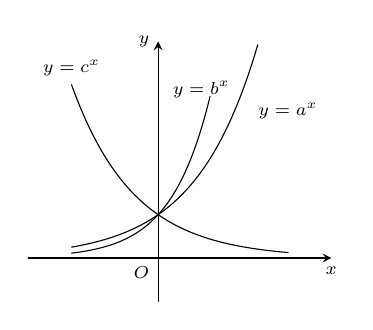
\begin{tikzpicture}[scale=0.55,font=\footnotesize,line join=round,line cap=round,>=stealth]
  \draw[->] (-3,0)  -- (4,0) node[below] {\scriptsize $x$};
  \draw[->] (0,-1) -- (0,5) node[left] {\scriptsize $y$}; 
  \draw (0,0) node[below  left]{\scriptsize $O$};
  \draw (3,3)  node[above]{\scriptsize $ y=a^x $};
  \draw (1,3.5) node[above]{\scriptsize $  y=b^x $};
  \draw (-2,4)  node[above]{\scriptsize $ y=c^x $};
  \draw[samples=150,smooth,domain=-2:2.3]  plot (\x,{2^(\x)});
  \draw[samples=150,smooth,domain=-2:1.2] plot  (\x,{3^(\x)});
  \draw[samples=150,smooth,domain=-2:3] plot (\x,{(0.5)^(\x)}); 
 \end{tikzpicture}
  }
 \choiceTF 
  {\True  $c^2 < 1$}
   {$a<1$}
   {$ab < 1$}
  {\True  $a+b-c > 0$}
 \loigiai{ 
  Kẻ đường thẳng $ x=1 $ cắt đồ thị  $ y=a^x $, $ y=b^x $ và $ y=c^x $ lần lượt tại các điểm $ A(1;a) $, $ B(1;b) $ và $ C(1;c) $.
  \begin{center}
   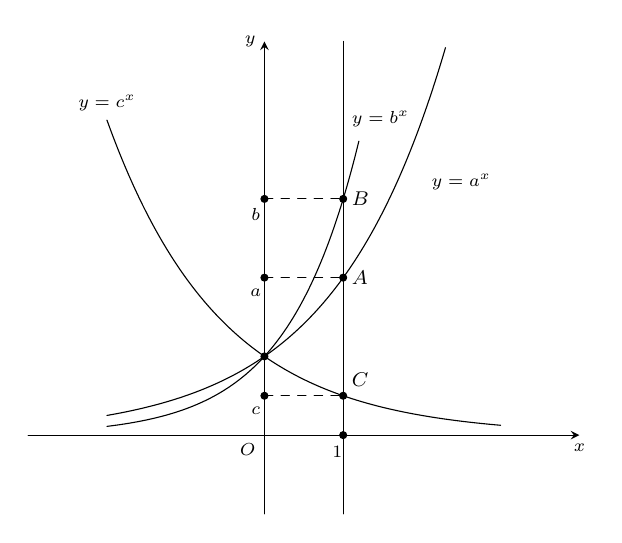
\begin{tikzpicture}[scale=1,font=\footnotesize,line join=round,line cap=round,>=stealth]
      \draw[->] (-3,0) -- (4,0) node[below] {\scriptsize $x$};
     \draw[->] (0,-1) -- (0,5) node[left] {\scriptsize  $y$};
     \draw (0,0) node[below  left]{\scriptsize $O$};
     \draw (2.5,3) node[above]{\scriptsize  $ y=a^x $};
     \draw (1,3.8) node[above right]{\scriptsize $ y=b^x  $};
     \draw (-2,4) node[above]{\scriptsize $  y=c^x $};
     \draw[samples=150,smooth,domain=-2:2.3] plot  (\x,{2^(\x)});
     \draw[samples=150,smooth,domain=-2:1.2] plot (\x,{3^(\x)}); 
     \draw[samples=150,smooth,domain=-2:3] plot (\x,{(0.5)^(\x)}); 
      \draw[fill=black] (1,2) circle (1.25pt) node[right]{$ A $}
      (1,3) circle (1.25pt) node[right]{$ B $} 
      (1,0.5) circle (1.25pt) node[above right]{$ C  $};
     \draw (1,-1)--(1,5); 
     \draw[dashed]  (0,0.5)--(1,0.5)
       (0,2)--(1,2)
      (0,3)--(1,3); 
     \foreach \x/\y in{1/0,0/1/2,0/2,0/3,0/0.5}\draw[fill=black](\x,\y)  circle (1.25pt);
     \foreach \x/\y/\goc/\z  in{1/0/-110/1,0/0.5/-120/c,0/2/-120/a,0/3/-120/b}
      \path (\x,\y) node[shift={(\goc:7pt)}]{\scriptsize$\z$};
    \end{tikzpicture}
  \end{center}
  Dựa vào đồ thị, ta có hàm số $ y=c^x $ nghịch biến trên $ \mathbb{R} $ nên $ 0<c<1 $ và hàm số $  y=a^x $, $ y=b^x $ đồng biến trên $ \mathbb{R} $ nên $ 1<a$, $b$.\\
  Mặt khác $ y_A<y_B $ nên $ a<b $.  Do đó $ 0<c<1<a<b $.
  \begin{itemchoice}
   \itemch \textbf{Đúng}. Vì $0 < c <1$ thì $c^2 < 1$. 
   \itemch \textbf{Sai}. 
    \itemch \textbf{Sai}. Vì $ab>1$
    \itemch\textbf{Đúng}.
  \end{itemchoice}
  }
\end{ex}

% từ: cau-hoi/lop11/1D6_Ham_so_mu_va_ham_so_logarit/1D6-3-3_Su_bien_thien_va_do_thi_cua_ham_so_mu_logarit.tex
\begin{ex}%[1D6V3-3]%[ma:cc624893]
	Cho đồ thị hàm số $ y=a^x$ dưới đây. 
	\begin{center}
		\begin{tikzpicture}[line join = round,line cap = round,>=stealth,font=\footnotesize,scale =1]
				\draw[->,line width  = 1pt] (-2,0)--(0,0) node[below right]{$O$}--(4.5,0) node[below]{$x$};
				\draw[->,line width = 1pt] (0,-1)--(0,4.5)  node[right]{$y$};
				\foreach \x  in {1} \draw[thin] (\x,2pt)--(\x,-2pt) node [below] {$\x$};
				\foreach \y in {1,3} \draw[thin]  (2pt,\y)--(-2pt,\y) node [left] {$\y$};
				\clip (-2,-1) rectangle  (3,4.5);
				\draw[samples=300,domain=-2.5:1.5,smooth] plot (\x,{(3)^(\x)}); 
				\draw[dashed]  (1,0)--(1,3)--(0,3);
				\fill[black] (1,3) circle (1pt); 
				 \path (2,4) node[below]{$y=a^x$};
			\end{tikzpicture}
	\end{center}
	\choiceTF 
		{Hàm  số đã cho nghịch biến trên khoảng $\left(0;1\right)$}
		{\True Hàm số cho bởi công thức  $ y=3^x$}
		{Đồ  thị hàm số đã cho cắt đường thẳng $ y=\dfrac{1}{3}$ tại điểm có hoành độ không âm}
		{Đồ thị hàm số đã  cho cắt đường thẳng $ y=-x+1$ tại điểm có hoành độ dương}
	\loigiai{ 
		\begin{itemchoice}
			\itemch SAI\\ 
			Dựa vào đồ thị hàm số ta thấy hàm số đã cho  đồng biến trên $ \mathbb{R} $
			 \itemch ĐÚNG\\
			 Đồ thị hàm số $ y=a^x$ đi qua điểm $ (1;3)$ suy ra $ a=3$.
			\itemch SAI\\ 
			Phương trình  hoành độ giao điểm của $ y=3^x$ và đường thẳng $ y=\dfrac{1}{3}$ là $3^x=\dfrac{1}{3}\Leftrightarrow x=-1$.
			\itemch SAI\\ 
			Phương trình hoành độ giao điểm của $ y=3^x$  và đường thẳng $ y=-x+1$ là $3^x=-x+1.\quad (1)$\\
			 Ta có hàm số $ y=3^x$ đồng biến trên $ \mathbb{R} $ và $ 3^x>0 $, $ \forall x \in \mathbb{R} $.\\
			Đường thẳng $ y=-x+1$ có hệ số  $ a=-1 < 0$ nên nghịch biến trên $ \mathbb{R} $.\\
			Ta lại có  $3^0=-0+1$ nên phương trình $ (1)$ có nghiệm duy nhất $ x=0$.
	\end{itemchoice}}
\end{ex}

% từ: cau-hoi/lop11/1D6_Ham_so_mu_va_ham_so_logarit/1D6-3-4_So_sanh_cac_luy_thua_va_logarit.tex
\begin{ex}%[1D6H3-4]%[ma:03b3a4fd]
 Cho $a$, $b$ là các  số thực.
  \choiceTF
  {\True $a >1$  nên $a^{\sqrt{2}} < a^{\sqrt{3}}$}
  {$0<a<1$ nên $\log_a 30 >  \log_a 29{,}7$}
  {$0 <  b < 1$ nên $b^{\tfrac{\sqrt{3}}{4}} < b^{\tfrac{\sqrt{2}}{3}}$}
  {\True $b>1$ nên $\log_b  7 > \log_b 2$}
 \loigiai{ 
  \begin{itemchoice}
   \itemch \textbf{Đúng}. Vì $a>1$ nên hàm số $y=a^x$ đồng biến trên $\mathbb{R}$  và $\sqrt{2} < \sqrt{3}$ nên $a^{\sqrt{2}} < a^{\sqrt{3}}$.
   \itemch \textbf{Sai}.  Vì $0<a<1$ nên hàm số $y = \log_a x$ nghịch biến trên $(0;+\infty)$ và $30 > 29{,}7$ nên $\log_a 30 < \log_a 29{,}7$.
   \itemch \textbf{Sai}. Vì $0<b<1$ nên hàm số $y=b^x$ nghịch biến trên $\mathbb{R}$ và $\dfrac{\sqrt{3}}{4} < \dfrac{\sqrt{2}}{3}$ nên $b^{\tfrac{\sqrt{3}}{4}} >  b^{\tfrac{\sqrt{2}}{3}}$.
   \itemch \textbf{Đúng}. Vì $b>1$ nên hàm số $y = \log_b x$ đồng biến trên $(0;+\infty)$ và $7 > 2$ nên  $\log_b 7 > \log_b 2$.
  \end{itemchoice}
  }
\end{ex}

% từ: cau-hoi/lop11/1D6_Ham_so_mu_va_ham_so_logarit/1D6-4-2_Phuong_trinh_mu_logarit_co_ban.tex
\begin{bt}%[1D6H4-2]%[ma:af30a31c]
% nguon: Archive/SP-4Phan-Dot3/Data/KNTT_1-OTHK2_De01.tex #4241

	Giải phương trình  $3 \mathrm{e}^{2x+4}=4$.
	\loigiai{
			Ta có $3\mathrm{e}^{2x+4}=4 \Leftrightarrow \mathrm{e}^{2x+4}=\dfrac{4}{3} \Leftrightarrow 2x+4=\ln \dfrac{4}{3} \Leftrightarrow x=\dfrac{1}{2} \ln \dfrac{4}{3}-2$.\\
			Vậy phương trình có nghiệm là $x=\dfrac{1}{2} \ln \dfrac{4}{3}-2$.
	}
\end{bt}

% từ: cau-hoi/lop11/1D6_Ham_so_mu_va_ham_so_logarit/1D6-4-3_Bat_phuong_trinh_mu_logarit_co_ban.tex
\begin{ex}%[1D6H4-3]%[ma:1ab556e6]
	Cho hàm số  $y=f(x)=\log_2 (x-3)$.
	\choiceTF 
		{\True Điểm $A(5;1)$  thuộc đồ thị hàm số $y=f(x)$}
		{\True  Tập xác định của hàm số $y=f(x)$ là $(3;+\infty)$}
		{Đồ thị hàm số $y=f(x)$ cắt đường thẳng $y=3$ tại điểm  có hoành độ $x=8$}
		{\True Có đúng ba điểm có hoành độ nguyên, thuộc đồ thị hàm số  $y=f(x)$ và $f(x)<2$}
	 \loigiai{
		\begin{itemchoice}
			\itemch Vì $f(5)=\log_2(5-3)=\log_2 2=1$ nên điểm  $A(5;1)$ thuộc đồ thị.
			\itemch Điều kiện  xác định $x-3>0\Leftrightarrow x>3$.\\
			Tập xác định $\mathscr{D}=(3;+\infty)$. 
			\itemch Phương trình hoành độ giao  điểm $\log_2 (x-3)=3\Leftrightarrow x-3=8\Leftrightarrow x=11$.
			\itemch Ta có $f(x)<2\Leftrightarrow \log_2 (x-3)<2\Leftrightarrow \heva{&x-3>0 \\&x-3<4}\Leftrightarrow  \heva{&x>3 \\&x<7.}$\\
			Mà $x\in \mathbb{Z}$ nên $x\in \{4;5;6\}$. 
		\end{itemchoice}
	 }
\end{ex}

% từ: cau-hoi/lop11/1D7_Dao_ham/1D7-1-2_So_gia_ham_so_so_gia_bien_so.tex
\begin{ex}%[1D7H1-2]%[ma:3d5924dd]
	Cho hàm số $y=f(x)$ có đạo hàm tại $x_0$ là $f'(x_0)$. Khẳng định nào sau  đây là \textbf{sai}?
	\choice 
		{\True  $f'(x_0)=\lim\limits_{x\to x_0}\dfrac{f(x+x_0)-f(x_0)}{x-x_0}$}
		{$f'(x_0)=\lim\limits_{x\to \Delta x}\dfrac{f(x_0+\Delta  x)-f(x_0)}{\Delta x}$}
		{$f'(x_0)=\lim\limits_{x\to  x_0}\dfrac{f(x)-f(x_0)}{x-x_0}$}
		{$f'(x_0)=\lim\limits_{h\to 0}\dfrac{f(h+x_0)-f(x_0)}{h}$} 
	\loigiai{ 
		Theo định nghĩa đạo  hàm của hàm số tại một điểm.\\
		Mệnh đề  $f'(x_0)=\lim\limits_{x\to x_0}\dfrac{f(x+x_0)-f(x_0)}{x-x_0}$ là mệnh đề sai
	 }
\end{ex}

% từ: cau-hoi/lop11/1D7_Dao_ham/1D7-1-4_Y_nghia_Vat_ly_cua_dao_ham.tex
\begin{bt}%[1D7V1-4]%[ma:63a79961]
% nguon: Archive/SP_DA_SauLuoi/1-TN-DS-TLN-THPT-ToanThang-HaiPhong-HKII-N23-24.tex #2456
%[Dự án đề kiểm tra Toán 11 HKII NH23-24-Dot-17-Lê Hữu Kiệt]%[THPT Toàn Thắng - Tỉnh Hải Phòng]
	\immini[thm]
	{Một vật chuyển động có vận tốc (m/s) được xác định bởi hàm số bậc hai có đồ thị như hình vẽ. Gia tốc tại thời điểm vận tốc bị triệt tiêu là $a\sqrt{b}$ (m/s$^2$) với $a>1$. Tính $2a+3b$.}
	{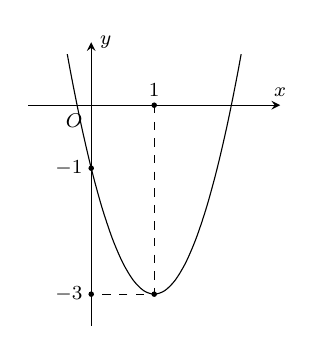
\begin{tikzpicture}[font=\footnotesize, >=stealth, x=0.8cm, y=0.8cm]
	\draw[->] (-1,0)--(3,0)node[above]{$x$};
	\draw[->] (0,-3.5)--(0,1)node[right]{$y$};
	\draw (0,0) node[below left]{$O$};
	\draw[dashed] (1,0) |- (0,-3);
	\begin{scope}
		\clip (-1,-3.5) rectangle (3,0.8);
		\draw[smooth] plot[domain=-1:3] (\x,{2*(\x)^2-4*(\x)-1});
	\end{scope}
	\fill[black]
		(0,-1) circle (1pt) node[left]{$-1$}
		(0,-3) circle (1pt) node[left]{$-3$}
		(1,0) circle (1pt) node[above]{$1$}
		(1,-3) circle (1pt)
		;
	\end{tikzpicture}}
	\par\shortans[]{$22$}
	\loigiai{
	Gọi $v(x)=mx^2+nx+q$ là hàm số vận tốc của vật ($m\ne 0$).
	\begin{itemize}
		\item Đồ thị hàm số đi qua điểm $(0;-1)$, suy ra $q=-1$.
		\item Đồ thị hàm số đi qua điểm $(1;-3)$, suy ra $m+n-1=-3 \Rightarrow m+n=-2$. \quad$(1)$
		\item Đồ thị hàm số có hoành độ đỉnh là $1$, suy ra $-\dfrac{n}{2m}=1 \Rightarrow 2m+n=0$. \quad$(2)$
	\end{itemize}
	Từ $(1)$ và $(2)$ ta có hệ phương trình $\heva{&m+n=-2 \\& 2m+n=0}\Leftrightarrow \heva{&m=2 \\& n=-4.} \quad\text{(thỏa mãn)}$\\
	Suy ra $v(x)=2x^2-4x-1$.\\
	Gọi $a(x)$ là hàm số gia tốc của vật, ta có $a(x)=v'(x)=4x-4$.\\
	Tại thời điểm vận tốc triệt tiêu, ta có $v(x)=0$ và $x> 0$.\\
	Ta có $v(x)=0 \Leftrightarrow 2x^2-4x-1=0 \Leftrightarrow \hoac{&x=\dfrac{2+\sqrt6}{2} \quad\text{(nhận)} \\& x=\dfrac{2-\sqrt6}{2}. \quad\text{(loại)}}$\\
	Khi đó $a\left(\dfrac{2+\sqrt6}{2}\right)=2\sqrt6$.\\
	Suy ra $a=2$; $b=6$. Vậy $2a+3b=22$.
	}
\end{bt}

% từ: cau-hoi/lop11/1D7_Dao_ham/1D7-2-8_Toan_thuc_te_ap_dung_quy_tac_dao_ham.tex
\begin{ex}%[1D7N2-8]%[ma:f5ab6bf9]
	Cho chuyển động được xác định bởi phương trình $S(t)=t^{3}-3t^{2}+t+11$, trong đó $t$ được tính bằng giây và $S$ được tính bằng mét. Vận tốc của chuyển động khi $t=2$  giây là
	\choice 
		{$9$ m/s} 
		 {$6$ m/s}
		 {$-3$ m/s}
		{\True $1$  m/s}
	 \loigiai{
		Ta có $S'(t)=3t^{2}-6t+1\Rightarrow  v(2)=S'(2)=1$.
	 }
\end{ex}

% từ: cau-hoi/lop11/1D7_Dao_ham/1D7-2-8_Toan_thuc_te_ap_dung_quy_tac_dao_ham.tex
\begin{ex}%[1D7H2-8]%[ma:52b75fa8]
	Cho chuyển động được xác định bởi phương trình $s=2t^3+6t^2-t$, trong đó $t$ được tính bằng giây và $s$ được tính bằng mét. Vận tốc tức thời của chuyển động tại thời điểm $t=3$  s là
	 \choice
		{\True $89$ m/s} 
		{$105$  m/s}
		{$48$  m/s}
		{$20$ m/s} 
	 \loigiai{
		Ta có  $v(t)=S'(t)=6t^2+12t-1$.\\
	Vận tốc tức  thời của chuyển động khi $t=3$ s là $v(3)=6\cdot 3^2+12\cdot 3-1=89$ m/s.}
\end{ex}

% từ: cau-hoi/lop11/1D7_Dao_ham/1D7-2-8_Toan_thuc_te_ap_dung_quy_tac_dao_ham.tex
\begin{ex}%[1D7H2-8]%[ma:b21706a8]
	Một vật  chuyển động theo quy luật $s(t)=-\dfrac{1}{2}t^3+12t^2$, $t$ (giây) là khoảng thời gian tính từ lúc vật bắt đầu chuyển động, $s$ (mét) là quãng đường vật chuyển động trong $t$ giây. Vận tốc tức thời của vật tại thời điểm $t=10$ (giây) là
	\choice 
		 {$80$ (m/s)}
		{\True  $90$ (m/s)}
		{$100$ (m/s)} 
		{$70$  (m/s)}
	\loigiai{ 
		Vận tốc tức thời  của vật tại thời điểm $t$ là $v\left(t\right)=s'(t)=-\dfrac{3}{2}t^2+24t$.\\
	Vận tốc tức thời của vật tại  thời điểm $t=10$ (giây) là $v\left(10\right)=-\dfrac{3}{2}\cdot10^2+24\cdot10=90$ (m/s).}
\end{ex}

% từ: cau-hoi/lop11/1D7_Dao_ham/1D7-2-8_Toan_thuc_te_ap_dung_quy_tac_dao_ham.tex
\begin{ex}%[1D7V2-8]%[ma:479ad685]
 Một vật chuyển động theo quy luật $s(t) = -\dfrac{1}{2} t^3 + 12t^2$, trong đó  $t$(giây) là khoảng thời gian tính từ lúc vật bắt đầu chuyển động, $s$ (mét) là quãng đường vật chuyển động được trong $t$ giây.
  \choiceTF
  {\True Sau $2$ giây kể từ lúc bắt đầu chuyển động, vật đi được quãng  đường là $44$ m}
  {\True Vận tốc tức thời của vật tại thời điểm $t =  10$ giây bằng $90$ m/s}
  {Vận tốc của vật có giá trị lớn  nhất tại thời điểm $t=10$ giây}
  {\True Vật dừng hẳn tại thời điểm $t=16$  giây}
  \loigiai{
 \begin{itemchoice}
  \itemch Sau $2$ giây kể từ lúc bắt đầu chuyển động, vật đi được quãng đường là $s(2)=  -\dfrac{1}{2} \cdot (2)^3 + 12\cdot (2)^2=44$ m.
  \itemch Biểu  thức vận tốc của vật là $v(t) = s'(t) = -\dfrac{3}{2}t^2 + 24 t$.\\
  Vận tốc tức thời của vật tại thời điểm $t = 10$ giây là $v(10)  = -\dfrac{3}{2} \cdot 10^2 + 24 \cdot 10 = 90 \textrm{ m/s}$.
  \itemch Ta có $v(t) = -\dfrac{3}{2}t^2 + 24 t=-\dfrac{3}{2}(t-8)^2+96\le  96$.\\
  Suy ra, vận tốc của vật có giá trị lớn nhất tại thời điểm $t=8$ giây. 
  \itemch Ta  có $v(t) = -\dfrac{3}{2}t^2 + 24 t=0\Rightarrow t=16$ giây.
 \end{itemchoice}
  }
\end{ex}

% từ: cau-hoi/lop11/1D7_Dao_ham/1D7-2-8_Toan_thuc_te_ap_dung_quy_tac_dao_ham.tex
\begin{ex}%[1D7H2-8]%[ma:bf8b5f8d]
	Một vật chuyển  động theo quy luật $s(t)=-\dfrac{1}{2}t^3+12t^2$, $t$ (giây) là khoảng thời gian tính từ lúc vật bắt đầu chuyển động, $s$ (mét) là quãng đường vật chuyển động trong $t$ giây. Vận tốc tức thời của vật tại thời điểm $t=10$ (giây) là
	 \shortans{90}
	\loigiai{ 
		Vận tốc tức thời của vật tại thời điểm $t$  là $v\left(t\right)=s'(t)=-\dfrac{3}{2}t^2+24t$.\\
	Vận tốc tức thời  của vật tại thời điểm $t=10$ (giây) là $v\left(10\right)=-\dfrac{3}{2}\cdot10^2+24\cdot10=90$ (m/s).}
\end{ex}

% từ: cau-hoi/lop11/1D7_Dao_ham/1D7-2-8_Toan_thuc_te_ap_dung_quy_tac_dao_ham.tex
\begin{ex}%[1D7V2-8]%[ma:4385acff]
	Một vật chuyển động thẳng xác định bởi phương trình $s(t)=-\dfrac{1}{3}t^3+3t^2+7t-2$, trong đó $t$ tính bằng giây và $s$ tính bằng mét. Vận tốc của vật đạt giá trị lớn nhất bằng bao  nhiêu?
	 \shortans{16}
	\loigiai{ 
		Ta có vận tốc của vật tại thời điểm $t$  là $v(t)=s'(t)=-t^2+6t+7$.\\
		Khi đó ta có $v(t)=-(t-3)^2+16\leq 16$ suy ra hàm số $v(t)$ đạt giá trị lớn nhất  bằng $16$ khi và chỉ khi $t-3=0\Leftrightarrow t=3$.\\
	Vậy vận tốc  của vật đạt giá trị lớn nhất bằng $16$ tại $t=3$.}
\end{ex}

% từ: cau-hoi/lop11/1D7_Dao_ham/1D7-3-3_Toan_thuc_te_va_Y_nghia_Vat_ly_cua_dao_ham_ca.tex
\begin{ex}%[1D7V3-3]%[ma:e38dc1e8]
	\immini{Một chuyển động có vận tốc được biểu diễn theo đồ thị là một đường parabol (xem hình bên). Tính gia tốc của chuyển động tại thời điểm $t=1$ s.}{\begin{tikzpicture}[scale=1,font=\footnotesize,line join=round,line cap=round,>=stealth,x=0.6cm,y=0.6cm,declare function = {f (\x) =-4*(\x)^2+11*(\x)+3;}]
		 \def \xmin{-1.5};
		\def \xmax{4.8}; 
		\def  \ymin{-1.5};
		\def  \ymax{11.5};
		\draw[->] (\xmin,0.) -- (\xmax,0.) node[anchor=north] {$t$}; 
		\draw[->]  (0.,\ymin) -- (0.,\ymax) node[anchor=west] {$v (t)$};
		\clip (\xmin+0.1,\ymin+0.1) rectangle  (\xmax-0.1,\ymax-0.1);
		\draw[smooth,samples=100,domain=0:3]  plot (\x,{f (\x)});
		\draw[dashed] (2,0) node[below]{$2$} |-  (0,9) node[left]{$9$};
		\foreach \x/\y/\l/\g in {0/0/O/225,3/0/3/-90,0/3/3/180,2/9//0}{\fill[black] (\x,\y) circle  (1pt)+(\g:0.5) node{$\l$};}
	\end{tikzpicture}
	 }
	\shortans{3} 
	\loigiai{ 
		 Đồ thị của vận tốc là một Parabol có phương trình $v(t)=at^2+bt+c$ ($a\neq 0$).\\
		Trên hình vẽ đồ thị qua các điểm $(0;3)$, $(2;9)$, $(3;0)$ nên ta  có hệ phương trình
		 $$\heva{&c=3\\&4a+2b+c=9\\&9a+3b+c=0}\Leftrightarrow\heva{&a=-4\\&b=11\\&c=3.}$$
		Do đó phương trình của vận  tốc là $v(t)=-4t^2+11t+3$.\\
		 Suy ra gia tốc của chuyển động là $a(t)=v'(t)=-8t+11$.\\
		Vậy gia tốc của chuyển động tại thời  điểm $t=1$ (s) là $a(1)=v'(1)=3$.
	 }
\end{ex}

% từ: cau-hoi/lop11/1H4_Duong_thang_mat_phang_Quan_he_song_song/1H4-3-2_Duong_thang_song_song_voi_mat_phang.tex
\begin{ex}%[1H4H3-2]%[ma:c14d7600]
	Cho hình lăng trụ tam giác  $ABC.A'B'C'$. Gọi $M$ và $M'$ lần lượt là trung điểm của các cạnh $BC$ và $B'C'$. Chứng minh rằng
	\begin{enumEX}{2}
		 \item $AA'\parallel\left(BCC'B'\right)$.
		 \item $AM\parallel A'M$.
	\end{enumEX}
	 \loigiai{
		\begin{center}
			\begin{tikzpicture}[line join=round,line cap=round,line width=.6pt,font=\footnotesize,scale=1]
					 \coordinate[label=left:$A$] (A) at (0,0);
					 \coordinate[label=below left:$B$] (B) at (1,-1);
					\coordinate[label=right:$C$] (C)  at (4,0);
					\coordinate (H)  at ($(B)!.5!(C)$);
					\coordinate[label=left:$A'$]  (A1) at ($(H)+(90:4)$);
					 \coordinate[label=left:$B'$] (B1) at ($(B)-(A)+(A1)$);
					\coordinate[label=right:$C'$] (C1) at  ($(C)-(A)+(A1)$);
					\coordinate[label=below:$M$]  (M) at ($(B)!1/2!(C)$);
					\coordinate[label=above:$M'$] (M1) at  ($(B1)!1/2!(C1)$);
					 \draw (A1)--(A)--(B)--(C)--(C1)--(A1)--(B1)--(C1)
						(B)--(B1) 
						 (A1)--(M1)--(M);
					\draw[dashed] (A)--(C) 
						(A)--(M); 
					\fill  (A) circle (1pt)
						(B) circle  (1pt)
						(C) circle  (1pt)
						 (A1) circle (1pt)
						 (B1) circle (1pt)
						(C1) circle (1pt) 
						(M)  circle (1pt)
						(M1) circle (1pt); 
				\end{tikzpicture}
		\end{center}
		\begin{enumerate}
			\item Trong hình lăng trụ $ABC.A'B'C'$ ta có $AA'\parallel BB'$ và $BB'\subset\left(BCC'B'\right)\Rightarrow  AA'\parallel\left(BCC'B'\right)$.
			\item Vì $MM'\parallel BB'$, $MM'=BB'$ và $BB'\parallel AA'$,  $BB'=AA'$ nên $MM'\parallel AA'$, $MM'=AA'$.\\
			Suy ra $AMM'A'$ là  hình bình hành nên $AM\parallel A'M'$.
	\end{enumerate} }
\end{ex}

% từ: cau-hoi/lop11/1H8_Quan_he_vuong_goc_trong_khong_gian/1H8-1-3_Tim_goc_giua_hai_duong_thang.tex
\begin{ex}%[1H8H1-3]%[ma:5b591150]
	Cho tứ diện $A B C D$ có $A B=A  C=2$, $D B=D C=3$. Khẳng định nào sau đây đúng?
	\choice 
		{\True $B C  \perp A D$}
		{$A C \perp B D$} 
		{$A B \perp(B C D)$} 
		{$D C \perp(A  B C)$}
	\loigiai{ 
		Do $A B=A C=2$,  $D B=D C=3$ nên $A$ và $D$ nằm trên mặt phẳng trung trực của $BC$.
		 \\
		Suy  ra $B C \perp A D$.
	 }
\end{ex}

% từ: cau-hoi/lop12/2D1_Ung_dung_dao_ham_de_khao_sat_ham_so/2D1-1-1_Xet_tinh_don_dieu_cua_ham_so_cho_boi_cong_thu.tex
\begin{ex}%[2D1H1-1]%[ma:11ba45bd]
	Cho hàm số $y=f(x)$ liên tục  trên $\mathbb{R}$ và có đạo hàm $f'(x)=(x+1)(x-1)^4(2-x)$. Mệnh đề nào dưới đây đúng?
	\choice 
		 {$f(5)>f(4)>f(3)$}
		 {$f(-1)>f(0)>f(1)$}
		 {$f(-3)<f(-2)<f(-1)$}
		{\True $f(0)<f(1)<f(2)$} 
	\loigiai{ 
		\begin{center}
			
\begin{tikzpicture}
				\tkzTabInit 
					 {$x$/1,$f'(x)$/1}
					{$-\infty$,$-1$,$1$,$2$,$+\infty$} 
				 \tkzTabLine{,-,0,+,0,+,0,-,}
			\end{tikzpicture}
		\end{center}
	Vì $f'(x)\geq 0\Leftrightarrow x\in (-1;2)$ nên hàm số đồng biến trên khoảng $(-1;2)$. \\ Do đó,  ta có $f(0)<f(1)<f(2)$.}
\end{ex}

% từ: cau-hoi/lop12/2D1_Ung_dung_dao_ham_de_khao_sat_ham_so/2D1-1-2_Xet_tinh_don_dieu_dua_vao_bang_bien_thien_do.tex
\begin{ex}%[2D1H1-2]%[ma:3b4138fd]
	Cho hàm  số $y=f(x)=\dfrac{ax^2+bx+c}{mx+n}$ (với $a, m\neq 0$) có đồ thị là~đường cong như hình
	\begin{center}
		\resizebox{!}{5cm}{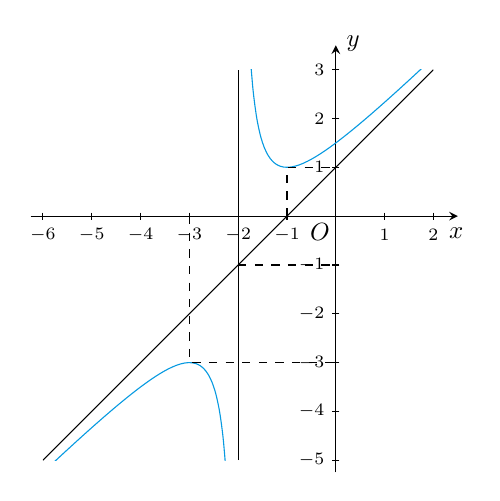
\begin{tikzpicture}[line cap=butt,line join=miter,>=stealth,xscale=0.62,yscale=0.62]
		 \tikzset{declare function={xmin=-6; xmax=2; Xkxd=-2;
			ymin=-5; ymax=3; 
			a=1; b=3; c=3; d=1;  et=2;
			akxd=1;  bkxd=1;
			f (\x)=(a*(\x)^2+b*\x+c)/(d*(\x)+et); 
			 h (\x)=akxd*\x+bkxd;
			 },
			 smooth,samples=50
		} 
		\draw[->]  (xmin-0.25,0)--(xmax+0.5,0)
			node[shift={(-95:7pt)},font=\normalsize]{$ x $}; 
		\draw[->]  (0,ymin-0.25)--(0,ymax+0.5)
			node[shift={(5:7pt)},font=\normalsize]{$ y $}; 
		\fill (0,0) node[shift={(225:9pt)},font=\normalsize]{$ O $}; 
		\foreach \x in  {-6,-5,-4,-3,-2,-1,1,2}{
			\draw (\x,2pt)--(\x,-2pt)  +(0,-9pt) node[font=\scriptsize,inner sep=1pt]{$\x$};
		 }
		\foreach  \y in {-5,-4,-3,-2,-1,1,2,3}{
			\draw (2pt,\y)--(-2pt,\y)  +(-3pt,0) node[font=\scriptsize,anchor=east,inner sep=1pt]{$\y$};
		} 
		\begin{scope}
			\clip (xmin,ymin) rectangle (xmax,ymax); 
			\draw (Xkxd,ymin)--(Xkxd,ymax); 
			\draw plot[domain=xmin:xmax]  (\x,{h (\x)});
			\draw[cyan!85!blue] plot[domain=xmin:{Xkxd-0.05}]  (\x,{f (\x)});
			 \draw[cyan!85!blue] plot[domain={Xkxd+0.05}:xmax] (\x,{f (\x)});
		\end{scope}
		\draw[dashed] (-3,0)--(-3,-3)--(0,-3) 
			(-1,0)--(-1,1)--(0,1) 
			(-2,-1)--(0,-1); 
	\end{tikzpicture}
		} 
	\end{center}
	 \choiceTF
		{\True Hàm số đồng  biến trên các khoảng $(-\infty;-3)$ và $(-1;+\infty)$}
		{\True $f(2024)  < f(2025)$}
		{Đồ thị  hàm số có tiệm cận đứng $x=-3$ và đường tiệm cận xiên $y=x+1$}
		{\True Đồ  thị hàm số đi qua điểm $A\left(2;\dfrac{13}{4}\right)$}
	 \loigiai{
		\begin{itemchoice}
			\itemch Nhìn đồ thị ta thấy mệnh  đề \textbf{đúng}.
			\itemch Do hàm số đồng biến trên khoảng  $(-1;+\infty)$, suy ra mệnh đề \textbf{đúng}.
			\itemch Nhìn đồ thị ta thấy đồ thị hàm số có tiệm cận đứng $x=-2$ và đường tiệm cận xiên đi qua  hai điểm $A\left(-1;0\right)$, $B\left(0;1\right)$ nên có phương trình $y=x+1$, suy ra mệnh đề \textbf{sai}.
			\itemch Ta thấy đồ thị hàm số có tiệm cận đứng $x=-2$ và đường tiệm cận xiên $y=x+1$. Dựa vào công thức thì đồ thị hàm số có tiệm cận đứng $x=-\dfrac{n}{m}$ và đường tiệm cận xiên $y=\dfrac{a}{m} x+\dfrac{b}{m}-\dfrac{an}{m^2}$. Từ đó suy  ra $\heva{&\dfrac{-n}{m}=-2 \\ &\dfrac{a}{m}=1 \\ &\dfrac{b}{m}-\dfrac{an}{m^2}=1}
			\Rightarrow \heva{&n=2m  \\ &a=m \\ &b=3m.}$\\
			 Do đó hàm số có dạng $y=f(x)=\dfrac{mx^2+3mx+c}{mx+2m}$.\\
			Đồ thị hàm số  đi qua điểm $M\left(-1;1\right)\Rightarrow 1=\dfrac{m-3m+c}{-m+2m} \Rightarrow c=3m$.\\
			Vậy hàm số có  dạng $y=f(x)=\dfrac{mx^2+3mx+3m}{mx+2m}=\dfrac{x^2+3x+3}{x+2}$.\\
			Ta  có $\dfrac{13}{4}=\dfrac{2^2+3\cdot2+3}{2+2}$ (đúng), nên đồ thị hàm số đi qua điểm $A\left(2;\dfrac{13}{4} \right)$, suy ra mệnh đề \textbf{đúng}.
		\end{itemchoice}
	} 
\end{ex}

% từ: cau-hoi/lop12/2D1_Ung_dung_dao_ham_de_khao_sat_ham_so/2D1-1-2_Xet_tinh_don_dieu_dua_vao_bang_bien_thien_do.tex
\begin{bt}%[2D1H1-2]%[ma:296d2b8f]
	 \immini{
	Cho đồ thị hàm số $y=f(x)$ có đồ thị như hình vẽ bên. Hàm số $y=f(x)$ nghịch biến trên khoảng $(a;b)$. Tính giá trị lớn nhất của  $b-a$.
	\shortans{2} 
	 }{
	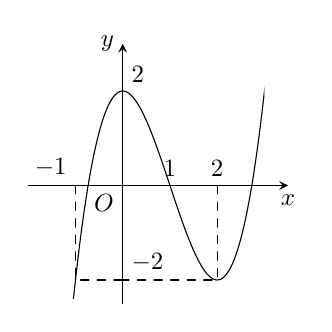
\begin{tikzpicture}[>=stealth,scale=0.6,line join=round,line cap=round]
		 \def\a{1} \def\b{-3} \def\c{0} \def\d{2}
		\def\xmin{-2} \def\xmax{3.5} \def\ymin{-2.5} \def\ymax{3} 
		\draw[->]  (\xmin,0)--(\xmax,0) node [below]{$x$};
		\draw[->] (0,\ymin)--(0,\ymax) node [left]{$y$}; 
		 \node at (0,0) [below left]{$O$};
		 \clip (\xmin+0.1,\ymin+0.1) rectangle (\xmax-0.5,\ymax-0.1);
		\draw[smooth,samples=300] plot  (\x,{\a*(\x)^3+\b*(\x)^2+\c*(\x)+\d});
		\draw[dashed](-1,0) node[above left]{$-1$}--(-1,-2)--(0,-2)  node[above right]{$-2$};
		\draw[dashed](2,0) node[above]{$2$}--(2,-2)--(0,-2); 
		\draw (1,0) node[above]{$1$};  \draw (0,2) node[above right]{$2$};
	\end{tikzpicture}
	 }
	 \loigiai{
		Dựa vào đồ thị hàm số ta thấy hàm số $y=f(x)$ nghịch biến trên  $(0;2)$.\\
		Suy ra $(a;b)\subset  (0; 2)$.\\
		Do đó $b-a$ lớn nhất khi $a=0$,  $b=2$.\\
		Vậy giá trị  lớn nhất của $b-a=2$.
	} 
\end{bt}

% từ: cau-hoi/lop12/2D1_Ung_dung_dao_ham_de_khao_sat_ham_so/2D1-1-2_Xet_tinh_don_dieu_dua_vao_bang_bien_thien_do.tex
\begin{bt}%[2D1N1-2]%[ma:8c7d75a6]
% nguon: Archive/2024/0. [LVH] BG - 12 New - 4in1-20240625T224301Z-001/0. [LVH] BG - 12 New - 4in1/2. [LVH] TEX SGK 12 NEW-20240418T074833Z-001/2. [LVH] TEX SGK 12 NEW/[LVH] CD-12new/SGK-12-CD/data/12-SGK-CD-1-1.tex #1074

	Cho hai hàm số $y=f(x)$, $y=g(x)$ có đồ thị lần lượt được cho ở \textit{Hình} $6a$, \textit{Hình} $6b$. Nêu khoảng đồng biến, nghịch biến và điểm cực trị của mỗi hàm số đó.
	\begin{center}
		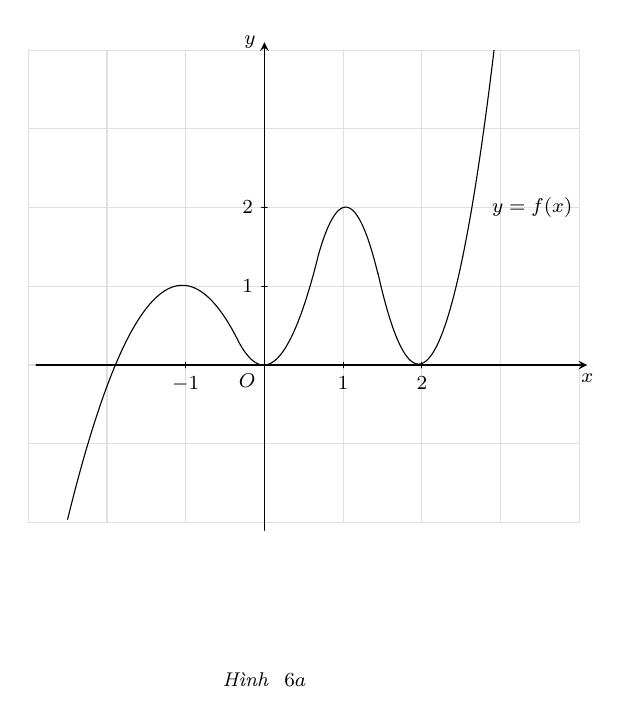
\begin{tikzpicture}[scale=1, font=\footnotesize, line join=round, line cap=round, >=stealth]
		\draw[gray!50,thin,opacity=.5] (-3,-2) grid (4,4);
		\draw[->] (-2.9,0)--(4.1,0) node[below] {$x$};
		\draw[->] (0,-2.1)--(0,4.1) node[left] {$y$};
		\draw (0,0) node [below left] {$O$};
		\foreach \x/\nx in {-1/-1,1/1,2/2}
		\draw[thin] (\x,1pt)--(\x,-1pt) node [below] {$\nx$};
		\foreach \y/\ny in {1/1,2/2}
		\draw[thin] (1pt,\y)--(-1pt,\y) node [left] {$\ny$};
		\begin{scope}
			\clip (-2.8,-2) rectangle (4,4);
			\draw[samples=200,domain=-2.5:-0.32,smooth,variable=\x] plot (\x,{-1.4*(\x)^2-2.92*(\x)-0.51});
			\draw[samples=200,domain=-0.32:0.68,smooth,variable=\x] plot (\x,{2.9*(\x)^2+0.05*(\x)});
			\draw[samples=200,domain=0.68:1.44,smooth,variable=\x] plot (\x,{-5.06*(\x)^2+10.44*(\x)-3.38});
			\draw[samples=200,domain=1.44:3.5,smooth,variable=\x] plot (\x,{4.34*(\x)^2-16.99*(\x)+16.64});
		\end{scope}
		\draw (3.4,2) node{$y=f(x)$};
		\draw (0,-4) node{\text{\textit{Hình }} $6a$};
	\end{tikzpicture}
	\hspace{0.5cm}
	\begin{tikzpicture}[scale=1, font=\footnotesize, line join=round, line cap=round, >=stealth]
		\draw[gray!50,thin,opacity=.5] (-3,-8.5) grid (3,1);
		\draw[->] (-3,0)--(3,0) node[below] {$x$};
		\draw[->] (0,-8.5)--(0,1) node[left] {$y$};
		\draw (0,0) node [above left] {$O$};
		\foreach \x/\nx in {-2/-2,1/1}
		\draw[thin] (\x,1pt)--(\x,-1pt) node [below] {$\nx$};
		\foreach \y/\ny in {-8/-8}
		\draw[thin] (1pt,\y)--(-1pt,\y) node [left] {$\ny$};
		\begin{scope}
			\clip (-3,-8.6) rectangle (2.9,1.2);
			\draw[samples=200,domain=-2.76:-1.75,smooth,variable=\x] plot (\x,{14.08*(\x)^2+55.22*(\x)+46.11});
			\draw[samples=200,domain=-1.75:0.54,smooth,variable=\x] plot (\x,{-2.4*(\x)^2+0.03*(\x)});
			\draw[samples=200,domain=0.54:1.9,smooth,variable=\x] plot (\x,{2.76*(\x)^2-5.48*(\x)+1.47});
		\end{scope}
	\draw[dashed,thin] (0,-1.25)node[left]{$-\tfrac{5}{4}$}--(1,-1.25);
	\draw (-1,-4) node[rotate=75]{$y=g(x)$};
	\draw (0,-9) node{\text{\textit{Hình }} $6b$};
	\end{tikzpicture}
	\end{center}
	\loigiai{
	\begin{itemize}
		\item Quan sát đồ thị \textit{Hình} $6a$, ta thấy hàm số $y=f(x)$ đồng biến trên các khoảng $(-\infty;-1)$, $(0;1)$, $(2;+\infty)$; nghịch biến trên các khoảng $(-1;0)$, $(1;2)$.\\
		Hàm số đạt cực đại tại $x=-1$, $x=1$ và đạt cực tiểu tại $x=0$, $x=2$.
		\item Quan sát đồ thị \textit{Hình} $6b$, ta thấy hàm số $y=g(x)$ đồng biến trên các khoảng $(-2;0)$, $(1;+\infty)$; nghịch biến trên các khoảng $(-\infty;-2)$, $(0;1)$.\\
		Hàm số đạt cực đại tại $x=0$ và đạt cực tiểu tại $x=-2$, $x=1$.
	\end{itemize} 
	}
\end{bt}

% từ: cau-hoi/lop12/2D1_Ung_dung_dao_ham_de_khao_sat_ham_so/2D1-1-2_Xet_tinh_don_dieu_dua_vao_bang_bien_thien_do.tex
\begin{bt}%[2D1N1-2]%[ma:09a5b63c]
% nguon: Archive/2024/0. [LVH] BG - 12 New - 4in1-20240625T224301Z-001/0. [LVH] BG - 12 New - 4in1/2. [LVH] TEX SGK 12 NEW-20240418T074833Z-001/2. [LVH] TEX SGK 12 NEW/[LVH] SGK-12-KNTT/data/C1/12-SGK-KNTT-1-1.tex #1114

	Tìm các khoảng đồng biến, khoảng nghịch biến của các hàm số có đồ thị như sau:
	\begin{center}
		\begin{tikzpicture}[scale=1,xscale=1.3, font=\footnotesize, line join=round, line cap=round, >=stealth]
			\draw[gray!50,thin,opacity=.5] (-2,-2) grid (3,3);
			\draw[->] (-1.6,0)--(2.6,0) node[below] {$x$};
			\draw[->] (0,-1.5)--(0,2.6) node[left] {$y$};
			\draw (0,0) node [above left] {$O$};
			\foreach \x/\nx in {-1/-1,1/1,2/2}
			\draw[thin] (\x,1pt)--(\x,-1pt) node [above] {$\nx$};
			\foreach \y/\ny in {1/1,2/2}
			\draw[thin] (1pt,\y)--(-1pt,\y) node [left] {$\ny$};
			\begin{scope}
				\clip (-2.8,-2) rectangle (4,4);
				\draw[samples=200,domain=-0.8:2,smooth,variable=\x] plot (\x,{(\x)^3-1.5*(\x)^2});
			\end{scope}
			\draw[dashed,thin] (0,-0.5)node[left]{$-\tfrac{1}{2}$}--(1,-0.5)--(1,0);
			\draw (1.2,0) node[below right]{$1,5$};
			\draw (0,3.4) node{\text{a) Đồ thị hàm số } $y=x^3-\dfrac{3}{2}x^2 \left(
				H.1.11\right)$ };
		\end{tikzpicture}
		\hspace{0.5cm}
		\begin{tikzpicture}[scale=1, font=\footnotesize, line join=round, line cap=round, >=stealth]
			\draw[gray!50,thin,opacity=.5] (-3,-1) grid (4,4);
			\draw[->] (-3,0)--(3.5,0) node[below] {$x$};
			\draw[->] (0,-1)--(0,3.5) node[left] {$y$};
			\draw (0,0) node [above left] {$O$};
			\foreach \x/\nx in {-2/-2,-1/-1,1/1,2/2,3/3}
			\draw[thin] (\x,1pt)--(\x,-1pt) node [below] {$\nx$};
			\foreach \y/\ny in {1/1,2/2,3/3}
			\draw[thin] (1pt,\y)--(-1pt,\y) node [left] {$\ny$};
			\begin{scope}
				%\clip (-3,-1) rectangle (2.9,1.2);
				\draw[samples=200,domain=-3:3,smooth,variable=\x] plot (\x,{(((\x)^2-4)^2)^(1/3)});
				%\draw[samples=200,domain=-1.999:1.999,smooth,variable=\x] plot (\x,{(((\x)^2-4)^2)^(1/3)});
				%\draw[samples=200,domain=2:3,smooth,variable=\x] plot (\x,{(((\x)^2-4)^2)^(1/3)});
			\end{scope}
			\draw[dashed,thin] (0,2.5)node[left]{$2,5$};
			\draw (0,3.85) node[above]{b) Đồ thị hàm số $y=\sqrt[3]{\left(x^2-4\right)^2} \left(H.1.12\right)$ };
			%\draw (0,-1) node{\text{\textit{Hình }} $6b$};
		\end{tikzpicture}
	\end{center}
	\loigiai{
		\begin{enumerate}[a)]
			\item Quan sát đồ thị \textit{Hình} $H.1.11$, ta thấy hàm số $y=x^3-\dfrac{3}{2}x^2$ đồng biến trên các khoảng $(-\infty;0)$,  $(1;+\infty)$; nghịch biến trên khoảng $(0;1)$.
			\item Quan sát đồ thị \textit{Hình} $H.1.12$, ta thấy hàm số $y=\sqrt[3]{\left(x^2-4\right)^2}$ đồng biến trên các khoảng $(-2;0)$, $(2;+\infty)$; nghịch biến trên các khoảng $(-\infty;-2)$, $(0;2)$.
		\end{enumerate} 
	}
\end{bt}

% từ: cau-hoi/lop12/2D1_Ung_dung_dao_ham_de_khao_sat_ham_so/2D1-1-4_Ung_dung_tinh_don_dieu_de_chung_minh_bat_dang.tex
\begin{bt}%[2D1V1-4]%[ma:292f25e6]
% nguon: Archive/2024/TaiLieuGiangDay/1.HamSo/1. K12 - 4in1 - Hamso/ThubaiGoc/Bai1-Dang4.tex #2657
[Mức độ 3]%[Dự án bài giảng new 4in1, Trần Quang Thạnh]
	Giải bất phương trình $ \log_2(2^x+1)+\log_3(4^x+2)\le 2$.\hfill $ (*) $
	\loigiai{
		\begin{itemize}
			\item Điều kiện $ \heva{&2^x+1>0\\&4^x+2>0} $ đúng $ \forall x\in \mathbb{R}\Rightarrow  $ Tập xác định $ \mathscr{D}=\mathbb{R} $.
			\item Xét hàm số $ f(x)=\log_2(2^x+1)+\log_3(4^x+2) $ trên $ \mathbb{R} $.\\
			Ta có $ f'(x)=\dfrac{2^x\ln2}{(2^x+1)\ln2}+\dfrac{4^x\ln4}{(4^x+1)\ln3}>0,\forall x\in \mathbb{R}\Rightarrow $ Hàm số $ y=f(x)  $ luôn đồng biến trên $ \mathbb{R} $.\\
			Ta có $ f(0)=2 $ do đó $ \forall x\le 0 $ thì $ f(x)\le f(0)\Leftrightarrow x\le0 $.
			\item Vậy tập nghiệm của bất phương trình là $ x\in (-\infty;0] $.
	\end{itemize}}
\end{bt}

% từ: cau-hoi/lop12/2D1_Ung_dung_dao_ham_de_khao_sat_ham_so/2D1-1-5_Toan_thuc_te_ung_dung_su_dong_bien_nghich_bie.tex
\begin{bt}%[2D1N1-5]%[ma:05e15f2f]
% nguon: Archive/2024/TaiLieuGiangDay/1.HamSo/1. K12 - 4in1 - Hamso/ThubaiGoc/Bai1-Dang5.tex #2668
[SGK12-CTST, Mức độ 1]%[BG12-4in1, Trần Thiên Đức]
	\immini{Trong $8$ phút kể từ khi xuất phát, độ cao $h$ (tính bằng mét) của khinh khí cầu vào tời điểm $t$ phút được cho bởi công thức $h(t)=6t^3-81t^2+324t$. Đồ thị của hàm số $h(t)$ được biểu diễn trong hình bên. Trong các khoảng thời gian nào khinh khí cầu tăng dần độ cao, giảm dần độ cao? Độ cao của khinh khí cầu vào các thời điểm $3$ phút và $6$ phút sau khi xuất phát có gì đặc biệt?
	}{
		\begin{tikzpicture}[scale=0.7, font=\footnotesize, line join=round, line cap=round, >=stealth]
			\def\xmin{-2} \def\xmax{9}
			\def\ymin{-1} \def\ymax{6} 
			\draw[->] (\xmin,0)--(\xmax,0) node [below]{$t$};
			\draw[->] (0,\ymin)--(0,\ymax) node [left]{$h$};
			\clip (\xmin+0.1,\ymin+0.1) rectangle (\xmax-0.1,\ymax-0.1);
			\draw[smooth,samples=300,domain=0:7.3,black] plot(\x,{0.07*(\x)^3-0.89*(\x)^2+3.39*(\x)});
			\fill (0,0)circle (1pt)node[below left]{$O$};
			\fill (0,3.35)circle(1pt )node[left]{$324$} (0,4.05)circle(1pt )node[left]{$405$} (0,4.6)circle(1pt )node[left]{$480$}
			(3,0)circle(1pt )node[below]{$3$}
			(5.6,0)circle(1pt )node[below]{$6$}
			(7.3,0)circle(1pt )node[below]{$8$}
			;
			\draw[dashed] (3,0)--(3,4.05)--(0,4.05) (5.6,0)--(5.6,3.35)--(0,3.35) (7.3,0)--(7.3,4.6)--(0,4.6);
			\fill (3,4.05)circle (1pt)
			(5.6,3.35)circle (1pt)
			(7.3,4.6)circle (1pt)
			;
		\end{tikzpicture}
	}
	\loigiai{
		Dựa vào đồ thị ta thấy khinh khí cầu tăng dần độ cao trong khoảng thời gian $3$ phút đầu và từ phút thứ $6$ đến phút thứ $8$, khinh khí cầu giảm dần độ cao trong khoảng thời gian từ phút thứ $3$ đến phút thứ $6$.\\
		Độ cao của khinh khí cầu tại thời điểm phút thứ $3$ là lớn nhất trong khoảng thời gian $6$ phút đầu, độ cao của khinh khí cầu tại thời điểm phút thứ $6$  là nhỏ nhất trong khoảng thời gian từ phút thứ $3$ đến phút thứ $8$.
		
	}
\end{bt}

% từ: cau-hoi/lop12/2D1_Ung_dung_dao_ham_de_khao_sat_ham_so/2D1-1-5_Toan_thuc_te_ung_dung_su_dong_bien_nghich_bie.tex
\begin{bt}%[2D1N1-5]%[ma:139c6fe4]
% nguon: Archive/2024/TaiLieuGiangDay/1.HamSo/1. K12 - 4in1 - Hamso/Thubai/Bai1-Dang5.tex #3041
%%[SGK12-CTST, Mức độ 1]%[BG12-4in1, Trần Thiên Đức]
	\immini{Trong $8$ phút kể từ khi xuất phát, độ cao $h$ (tính bằng mét) của khinh khí cầu vào tời điểm $t$ phút được cho bởi công thức $h(t)=6t^3-81t^2+324t$. Đồ thị của hàm số $h(t)$ được biểu diễn trong hình bên. Trong các khoảng thời gian nào khinh khí cầu tăng dần độ cao, giảm dần độ cao? Độ cao của khinh khí cầu vào các thời điểm $3$ phút và $6$ phút sau khi xuất phát có gì đặc biệt?
	}{
		\begin{tikzpicture}[scale=0.7, font=\footnotesize, line join=round, line cap=round, >=stealth]
			\def\xmin{-2} \def\xmax{9}
			\def\ymin{-1} \def\ymax{6} 
			\draw[->] (\xmin,0)--(\xmax,0) node [below]{$t$};
			\draw[->] (0,\ymin)--(0,\ymax) node [left]{$h$};
			\clip (\xmin+0.1,\ymin+0.1) rectangle (\xmax-0.1,\ymax-0.1);
			\draw[smooth,samples=300,domain=0:7.3,black] plot(\x,{0.07*(\x)^3-0.89*(\x)^2+3.39*(\x)});
			\fill (0,0)circle (1pt)node[below left]{$O$};
			\fill (0,3.35)circle(1pt )node[left]{$324$} (0,4.05)circle(1pt )node[left]{$405$} (0,4.6)circle(1pt )node[left]{$480$}
			(3,0)circle(1pt )node[below]{$3$}
			(5.6,0)circle(1pt )node[below]{$6$}
			(7.3,0)circle(1pt )node[below]{$8$}
			;
			\draw[dashed] (3,0)--(3,4.05)--(0,4.05) (5.6,0)--(5.6,3.35)--(0,3.35) (7.3,0)--(7.3,4.6)--(0,4.6);
			\fill (3,4.05)circle (1pt)
			(5.6,3.35)circle (1pt)
			(7.3,4.6)circle (1pt)
			;
		\end{tikzpicture}
	}
	\loigiai{
		Dựa vào đồ thị ta thấy khinh khí cầu tăng dần độ cao trong khoảng thời gian $3$ phút đầu và từ phút thứ $6$ đến phút thứ $8$, khinh khí cầu giảm dần độ cao trong khoảng thời gian từ phút thứ $3$ đến phút thứ $6$.\\
		Độ cao của khinh khí cầu tại thời điểm phút thứ $3$ là lớn nhất trong khoảng thời gian $6$ phút đầu, độ cao của khinh khí cầu tại thời điểm phút thứ $6$  là nhỏ nhất trong khoảng thời gian từ phút thứ $3$ đến phút thứ $8$.
		
	}
\end{bt}

% từ: cau-hoi/lop12/2D1_Ung_dung_dao_ham_de_khao_sat_ham_so/2D1-1-5_Toan_thuc_te_ung_dung_su_dong_bien_nghich_bie.tex
\begin{bt}%[2D1V1-5]%[ma:1739d5ce]
% nguon: Archive/SP_SauLuoi_2024-2025/SP_HKI/2-TN-DS-TLN-THPT-GiaDinh-TPHCM-HKI-NH24-25.tex #142
%[Dự án A đợt 5,Nguyễn Tài Tuệ]%[THPT Gia Định, TPHCM]
	Vị trí của một vật chuyển động $s(t)$ (tính theo mét) vật đi được sau khoảng thời gian $t$ (tính theo giây), $t \geq 0$, được mô tả là một hàm số bậc ba có đồ thị như hình vẽ dưới đây.
	\begin{center}
		\begin{tikzpicture}[line join=round, line cap=round,>=stealth,thick,yscale=0.25,xscale=0.5]
			\tikzset{every node/.style={scale=0.9}}
			\draw[->] (-1.1,0)--(10.1,0) node[below] {$t(s)$};
			\draw[->] (0,-1.1)--(0,22.1) node[right] {$s(t)$ m};
			\draw (0,0) node [below left] {$O$};
			\draw[dashed] (3,0) node[below]{$3$}--(3,9)--(0,9) node[left]{$9$}  (7,0)node[below]{$7$} --(7,35/3)--(0,35/3) node[left]{$\tfrac{35}{3}$} (8,0) node[below]{$8$}--(8,52/3)--(0,53/3) node[left]{$\tfrac{52}{3}$};
			\begin{scope}
				\clip (-1,-1) rectangle (10,20);
				\draw[samples=200,domain=0:8.5,smooth,variable=\x] plot (\x,{1/6*((\x)^3)+-2*((\x)^2)+15/2*(\x)+0});
			\end{scope}
		\end{tikzpicture}
	\end{center}
	Trong $30$ giây đầu tiên, vật chuyển động nhanh dần bắt đầu từ thời điểm giây thứ mấy?\par
	\shortans{$3$}
	\loigiai{
		Gọi $s(t)=a t^3+b t^2+c t+d \quad(a \neq 0)$.\\
		Đồ thị hàm số $s(t)$ đi qua các điểm $O,(3 ; 9)$, $\left(7 ; \dfrac{35}{3}\right)$, $\left(8 ; \dfrac{52}{3}\right)$. 		
		$$
		\Rightarrow s(t)=\dfrac{1}{6}t^3-2 t^2+\dfrac{15}{2}t.
		$$
		Vật chuyển động nhanh dần nghĩa là vận tốc và gia tốc cùng dấu\\
		Xét vận tốc $v(t)=s'(t)=\dfrac{1}{2}t^2-4 t+\dfrac{15}{2}$ với $t \in[0 ; 30]$.\\
		$ v(t)=0 \Leftrightarrow \hoac{&t=3\\&t=5.}$\\
		Xét gia tốc $a(t)=v'(t)=t-4=0 \Leftrightarrow t=4$.\\
		Lập bảng xét dấu
		\begin{center}
			\begin{tabular}{|c|cccccccc|}
				\hline $t$ & $0$ & & $3$ & & $4$ & & $5$ & \\
				\hline Vận tốc $v(t)$ & & + & $0$ & - & $\mid$ & - & $0$ & + \\
				\hline Gia tốc $a(t)$ & & - & $\mid$ & - & $0$ & + & $\mid$ & + \\
				\hline$v(t) \cdot a(t)$ & & - & $0$ & + & $0$ & - & $0$ & + \\
				\hline
			\end{tabular}		 
		\end{center}
		Chuyển động nhanh dần từ giây thứ $3$.}
\end{bt}

% từ: cau-hoi/lop12/2D1_Ung_dung_dao_ham_de_khao_sat_ham_so/2D1-2-2_Tim_cuc_tri_dua_vao_BBT_do_thi.tex
\begin{ex}%[2D1N2-2]%[ma:802f411b]
	Cho hàm số bậc ba có đồ thị là đường cong trong hình  bên dưới.
	\begin{center}
		\begin{tikzpicture}[scale=1,font=\footnotesize,line join=round,line cap=round,>=stealth]
			 \draw[->] (-1,0)--(5,0) node[below] {$x$};
			 \draw[->] (0,-3)--(0,3) node[left] {$y$};
			\draw (0,0) node [below left]  {$O$};
			\fill (1,0) circle (1pt)  node[below] {$1$}
				(3,0) circle (1pt) node[above] {$3$}; 
			 \draw[dashed] (1,0)--(1,2)
				 (0,2)--(1,2)
				(3,0)--(3,-2) 
				 (0,-2)--(3,-2);
			\foreach  \y in {-2,2} \fill (0,\y) circle (1pt) node[left] {$\y$};
			\draw[smooth,samples=200] plot[domain=-0.11:4.1]  (\x,{\x^3-6*\x^2+9*\x-2});
		\end{tikzpicture}
	\end{center}
	Giá trị cực tiểu của hàm số  đã cho là
	\choice 
		{\True  $-2$}
		{$2$} 
		 {$1$}
		 {$3$}
	\loigiai{ 
		Giá trị cực tiểu  của hàm số đã cho là $-2$.
	 }
\end{ex}

% từ: cau-hoi/lop12/2D1_Ung_dung_dao_ham_de_khao_sat_ham_so/2D1-3-1_GTLN_GTNN_tren_doan.tex
\begin{ex}%[2D1N3-1]%[ma:fb34898f]
	\immini{Một trong bốn đưởng thẳng dưới đây lả đưởng tiệm cận ngang của đồ thị hàm sổ ở hình bên. Hỏi đường tiệm cận ngang  của đồ thị hàm số đó là đường nào?
	 \choice
		{$x=-1$} 
		{$x=-2$} 
		{\True  $y=1$}
		{$y=2$}} 
		{\resizebox{!}{5cm}{\begin{tikzpicture}[line join=round,line cap=round,>=stealth,scale=0.6]
		\draw[gray!20](-5,-5)  grid (5,5);
		\draw[->] (-5.1,0)--(5.1,0) node[below left] {$x$}; 
		\draw[->] (0,-5)--(0,5) node[below  left] {$y$};
		\draw (0,0)  node [below left] {\footnotesize $O$};
		\foreach \x in  {-3,-2,-1,1,2,3}
		\draw[thin] (\x,1pt)--(\x,-1pt) node [below]  {\footnotesize $\x$};
		\foreach \y  in {-3,-2,-1,1,2,3}
		\draw[thin] (1pt,\y)--(-1pt,\y) node [left] {\footnotesize $\y$}; 
		\begin{scope}
			\clip (-5,-5)  rectangle (5,5);
			 \draw[samples=100,domain=-5:-1.1,smooth,variable=\x]
				plot  (\x,{((\x)+2)/((\x)+1)});
			\draw[samples=100,domain=-0.9:5,smooth,variable=\x] 
				 plot (\x,{((\x)+2)/((\x)+1)});
			\draw[samples=100,domain=-5:5,smooth,dashed,variable=\x] 
				plot (\x,{1/1}); 
			\draw[dashed]  (-1/1,-5)--(-1/1,5);
		\end{scope}
	\end{tikzpicture}
		 }}
	 \loigiai{
		Vì $\lim\limits_{x \to -\infty  } f(x)= 1$; $\lim\limits_{x \to +\infty } f(x)=1$. Nên đồ thị hàm số có tiệm cận ngang là $y=1$.
	} 
\end{ex}

% từ: cau-hoi/lop12/2D1_Ung_dung_dao_ham_de_khao_sat_ham_so/2D1-3-1_GTLN_GTNN_tren_doan.tex
\begin{ex}%[2D1H3-1]%[ma:a10a1757]
	\immini 
	{Đồ thị sau là của hàm số nào sau đây? 
	 \choice
		 {$\dfrac{2x^2+3}{5x^2-15x+10}$}
		{$\dfrac{2x-3}{x^2-5x+6}$} 
		{\True  $\dfrac{2x-3}{5x^2-15x+10}$}
		{$\dfrac{2x-3}{x^2+x-6}$} 
		 }
		{\begin{tikzpicture}[>=stealth,scale=0.7]
		\draw[->]  (-2,0) --(4,0);
		\draw[->](0,-4)--(0,3); 
		\draw (0,0.5)  node[above left]{$O$};
		\draw (4,0) node[below]{$x$}; 
		 \draw (0,3) node[left]{$y$};
		\draw (1,0) node[above left]{$1$}; 
		\draw (2,0) node[above  left]{$2$};
		\clip (-2,-4)  rectangle (4,3);
		\draw[samples=100]  plot[domain=-2:4]
			(\x,{(2*(\x)-3)/(5*(\x)^(2)-15*\x+10)}); 
		\draw (2.6,-1.5) node {\scriptsize  $x=2$};
		 \draw (0.2,-3.2) node {\scriptsize $x=1$};
	\end{tikzpicture}
		} 
	\loigiai{Dựa vào đồ thị hàm số ta thấy phương trình hai tiệm cận đứng là $x=1$ và $x=2$.\\ 
		Mặt khác đồ thị hàm số có đường tiệm  cận ngang là đường thẳng $y=0$.\\
		Vậy đồ thị là của hàm số $\dfrac{2x -  3}{5x^2-15x+10}$.
	 }
\end{ex}

% từ: cau-hoi/lop12/2D1_Ung_dung_dao_ham_de_khao_sat_ham_so/2D1-3-1_GTLN_GTNN_tren_doan.tex
\begin{ex}%[2D1V3-1]%[ma:354bc032]
	Cho hàm số $f(x)=\cos 2x-x$. 
	 \choiceTF
		{\True $f\left(-\dfrac{\pi}{2}\right)=\dfrac{\pi}{2}-1$; $f\left(\dfrac{\pi}{2}\right)=-\dfrac{\pi}{2}-1$} 
		{Đạo hàm của hàm số đã cho là  $f'(x)=2\sin 2x-1$}
		{Phương trình $f'(x)=0$ có đúng hai nghiệm trên đoạn $\left[-\dfrac{\pi}{2}; \dfrac{\pi}{2}\right]$  là $x=-\dfrac{\pi}{12}$ và $x=\dfrac{5\pi}{12}$}
		{\True Giá trị nhỏ nhất  của hàm số $y=f(x)$ trên đoạn $\left[-\dfrac{\pi}{2}; \dfrac{\pi}{2}\right]$ là $-\dfrac{\pi}{2}-1$}
	\loigiai{ 
		\begin{itemchoice}
			\itemch  \textbf{Đúng}.\\
			$f\left(-\dfrac{\pi}{2}\right)=\cos (-\pi)+\dfrac{\pi}{2}=\dfrac{\pi}{2}-1$.\\ $f\left(\dfrac{\pi}{2}\right)=\cos (\pi)-\dfrac{\pi}{2}=-\dfrac{\pi}{2}-1$ 
			\itemch  \textbf{Sai}.\\
			Đạo hàm  của hàm số đã cho là $f'(x)=-2\sin 2x-1$.
			\itemch  \textbf{Sai}.\\
			Ta có $f'(x)=-2\sin 2x-1=0\Leftrightarrow \sin 2x=-\dfrac{1}{2}\Leftrightarrow  \hoac{&x=-\dfrac{\pi}{12}+k\pi\\&x=\dfrac{7\pi}{12}+k\pi}, k\in \mathbb{Z}$.\\
			Vì $x\in  \left[-\dfrac{\pi}{2}; \dfrac{\pi}{2}\right]$ nên $x\in \left\{-\dfrac{\pi}{12};-\dfrac{5\pi}{12}\right\}$.\\
			\itemch \textbf{Đúng}.\\ 
			Ta  có $f\left(-\dfrac{\pi}{2}\right)=\dfrac{\pi}{2}-1$.\\
			 $f\left(\dfrac{\pi}{2}\right)=-\dfrac{\pi}{2}-1$.\\
			$f\left(-\dfrac{\pi}{12}\right)=\dfrac{\pi}{12}+\dfrac{\sqrt{3}}{2}$.\\ 
			 $f\left(-\dfrac{5\pi}{12}\right)=\dfrac{5\pi}{12}-\dfrac{\sqrt{3}}{2}$.\\
			Vậy  giá trị nhỏ nhất của hàm số $y=f(x)$ trên đoạn $\left[-\dfrac{\pi}{2}; \dfrac{\pi}{2}\right]$ là $-\dfrac{\pi}{2}-1$.
		\end{itemchoice}
	 }
\end{ex}

% từ: cau-hoi/lop12/2D1_Ung_dung_dao_ham_de_khao_sat_ham_so/2D1-3-4_Ung_dung_GTNN_GTLN_trong_bai_toan_phuong_trin.tex
\begin{bt}%[2D1N3-4]%[ma:fb80c3f5]
% nguon: Archive/2024/TaiLieuGiangDay/1.HamSo/1. K12 - 4in1 - Hamso/ThubaiGoc/Bai3-Dang6.tex #2021
[Mức độ 1]%[BG12-4IN1, Nguyễn Khánh Trọng]
	\immini{Cho hàm số $y=f(x)=\log_2x$ có đồ thị như hình vẽ bên. Tìm tất cả giá trị của tham số $m$ để bất phương trình $f(x)\ge m$ có nghiệm $x\in(0;4)$.
	}{\begin{tikzpicture}[line join=round,line cap=round,>=stealth,scale=0.5,font=\footnotesize]
		\def \xmin{-1} 		\def \xmax{6}
		\def \ymin{-1} 		\def \ymax{3.5}
		\def \fx{ln(\x)/ln(2)}
		\draw[->] (\xmin,0)--(\xmax,0) node[below left] {\normalsize$x$};
		\draw[->] (0,\ymin)--(0,\ymax) node[below left] {\normalsize$y$};
		\draw (0,0) node[below left] {$O$};
		\foreach \x in {1,4} \fill (\x,0) circle (1.25pt) node[below] {$\x$};
		\foreach \y in {2} \fill (0,\y) circle (1.25pt) node[left] {$\y$};
		\draw[dashed] (4,0)--(4,2)--(0,2);
		\begin{scope}
			\clip (\xmin+0.01,\ymin+0.01) rectangle (\xmax-0.01,\ymax-0.01);
			\draw[thick,samples=150,domain=0.1:\xmax-0.01,smooth,variable=\x] plot (\x,{\fx});
		\end{scope}
		\end{tikzpicture}}
	\loigiai{
		Ta có bất phương trình $f(x)\ge m$ có nghiệm $x\in(0;4)$ khi và chỉ khi
		$$f(4)> m\Leftrightarrow m<2.$$
	}	
\end{bt}

% từ: cau-hoi/lop12/2D1_Ung_dung_dao_ham_de_khao_sat_ham_so/2D1-3-6_Toan_thuc_te_ung_dung_GTLN_GTNN_cua_ham_so.tex
\begin{bt}%[2D1H3-6]%[ma:d7f60989]
	Một chất điểm chuyển động có quãng đường được cho bởi phương trình $s(t)=\dfrac{1}{6}t^4-\dfrac{4}{3}t^3+5t^2-7$, trong đó $t>0$ với $t$ tính bằng giây $(s)$, $s(t)$ tính bằng mét $(m)$. Vận tốc  chuyển động của chất điểm tại thời điểm chất điểm có gia tốc chuyển động nhỏ nhất là $\dfrac{a}{b}$ với $a$, $b \in \mathbb{Z}$ và $\dfrac{a}{b}$ là phân số tối giản. Tính $T=2a-3b$.
	\shortans{47} 
	 \loigiai{Phương trình vận tốc của chuyển động là $v(t)=s'(t)=\dfrac{2}{3}t^3-4t^2+10t$.\\
		Phương trình gia tốc  của chuyển động là $a(t)=v'(t)=2t^2-8t+10$.\\
		Ta có  $a'(t)=4t-8$.\\
		$a'(t)=0 \Leftrightarrow 4t-8 =0  \Leftrightarrow t=2$.\\
		Bảng biến thiên 
		\begin{center}
			\begin{tikzpicture}
				 \tkzTabInit[lgt=1.2,espcl=2]
					{$t$ /0.8,$a'(t)$ /0.8,$a  (t)$/2}
					{$0$,$2$,$+\infty$} 
				 \tkzTabLine{,-,z,+,}
				 \tkzTabVar{+/$+\infty$,-/$a (2)$,+/$+\infty$}
			\end{tikzpicture}
		\end{center}
		Dựa vào bảng biến thiên, ta có $\min \limits_{(0;+\infty)}=a(2)$ nên tại thời điểm $t=2$ vật có gia tốc chuyển  động nhỏ nhất.\\
		Vận tốc chuyển động của chất điểm tại thời điểm chất điểm có gia  tốc chuyển động nhỏ nhất là $v(2)=\dfrac{2}{3} \cdot 2^3 - 4 \cdot 2^2+10 \cdot 2=\dfrac{28}{3}$.\\
	Vậy  $a=28$, $b=3$ nên $T=2a-3b=2 \cdot 28- 3 \cdot 3=47$. }
\end{bt}

% từ: cau-hoi/lop12/2D1_Ung_dung_dao_ham_de_khao_sat_ham_so/2D1-4-1_Bai_toan_xac_dinh_cac_duong_tiem_can_cua_ham.tex
\begin{ex}%[2D1N4-1]%[ma:f5665ad2]
	 \immini{
	Cho hàm số $f(x)=\dfrac{ax+b}{cx+d}$ ($a$, $b$, $c$, $d\in \mathbb{R}$, $c\neq 0$) có đồ thị  như hình bên. Đường tiệm cận đứng của đồ thị hàm số là
	 \choice
		{$y=-2$} 
		 {$y=2$}
		 {$x=-2$}
		{\True $x=2$} 
		} 
		{ 
		\begin{tikzpicture}[scale=0.4,font=\footnotesize,line join=round,line cap=round,>=stealth]
			\draw[->] (-6.1,0)--(8.1,0) node[below left] {$x$}; 
			\draw[->] (0,-7.1)--(0,7.1) node[below  left] {$y$};
			\draw (0,0) node [below left] {$O$} circle (1pt); 
			\draw (2,0) node [below left] {$2$} circle (1pt); 
			 \draw (-2,0) node [below] {$-2$} circle (1pt);
			 \draw (0,2) node [right] {$2$} circle (1pt);
			\draw (0,-2) node [right] {$-2$} circle (1pt); 
			 \draw[dashed] (2.01,-7)--(2.01,7);
			\begin{scope}
				\clip  (-7,-7) rectangle (8,7);
				\draw[samples=100,domain=-6:1.9,smooth,variable=\x] plot (\x,{(0*(\x)+6)/((\x)+-2)}); 
				\draw[samples=100,domain=2.1:8,smooth,variable=\x]  plot (\x,{(0*(\x)+6)/((\x)+-2)});
				 \draw (-6,0/1)--(6,0/1);
			\end{scope}
		\end{tikzpicture}
		} 
	 \loigiai{
		Từ  đồ thị suy ra đường tiệm cận đứng là $x=2$.
	 }
\end{ex}

% từ: cau-hoi/lop12/2D1_Ung_dung_dao_ham_de_khao_sat_ham_so/2D1-4-1_Bai_toan_xac_dinh_cac_duong_tiem_can_cua_ham.tex
\begin{ex}%[2D1N4-1]%[ma:1cb19f38]
	\immini{Cho hàm số $y=f(x)$ có đồ thị  như hình bên. Đường tiệm cận ngang của đồ thị hàm số là
	\choice 
		{$x=-1$} 
		{$x=-2$} 
		{\True $y=1$} 
		{$y=2$}} 
		{\begin{tikzpicture}[scale=0.85,font=\footnotesize,line join=round,line cap=round,>=stealth]
		 \draw[->] (-3.75,0)--(2.75,0) node[above] {$x$};
		\draw[->] (0,-3)--(0,5.75) node[right] {$y$}; 
		\draw (0,0) node [below left] {$O$}; 
		\foreach \x in {1,2}\draw  (\x,0.1)--(\x,-0.1) node[below] {$\x$};
		\draw (-1,0.1)--(-1,-0.1) node[above  left] {$-1$};
		\draw (-2,0.1)--(-2,-0.1) node[below  left] {$-2$}
			(-3,0.1)--(-3,-0.1) node[below left] {$-3$}; 
		\foreach \y in {-2,-1,2,3,4,5}\draw  (-0.1,\y)--(0.1,\y) node[right] {$\y$};
		\draw (-0.1,1)--(0.1,1) node[above  right] {$1$};
		 \draw[dashed] (-3.75,1)--(2.5,1)
			 (-1,-3)--(-1,5.75);
		\draw[smooth,samples=200] plot[domain=-3.7:-1.25]  (\x,{(\x+2)/(\x+1)});
		 \draw[smooth,samples=200] plot[domain=-0.785:2] (\x,{(\x+2)/(\x+1)});
	\end{tikzpicture}
		 }
	\loigiai{ 
		Dựa vào  đồ thị của hàm số $y=f(x)$, ta có đường tiệm cận ngang của đồ thị hàm số là $y=1$.
	} 
\end{ex}

% từ: cau-hoi/lop12/2D1_Ung_dung_dao_ham_de_khao_sat_ham_so/2D1-4-3_Bai_toan_lien_quan_den_do_thi_ham_so_va_cac_d.tex
\begin{ex}%[2D1H4-3]%[ma:2d40d4d7]
	Cho hàm số $y=x^3-3x^2+1$.  Khi đó
	\choiceTF 
		{\True  Hàm số đồng biến trên mỗi khoảng $\left(-\infty;0\right)$ và $\left(2;+\infty \right)$}
		{\True Hàm số đạt cực tiểu tại điểm  $x=2$}
		{\True Bảng biến thiên của  hàm số là \\
		\begin{tikzpicture}[>=stealth]
			\tkzTabInit[nocadre=false,lgt=1,espcl=2,deltacl=0.5]{$x$/.7,$y'$/.7,$y$/2} 
				 {$-\infty$,$0$,$2$,$+\infty$}
			\tkzTabLine{,+,$0$,-,$0$,+,} 
			\tkzTabVar{-/$-\infty$,+/$1$,-/$-3$,+/$+\infty$} 
		\end{tikzpicture}
		 }
		{Đồ thị hàm  số nhận điểm $I\left(1;-2\right)$ làm tâm đối xứng}
	 \loigiai{
		\begin{itemchoice}
			 \itemch
			Tập  xác định $\mathscr{D}=\mathbb{R}$
			\[y'=3x^2-6x=0\Leftrightarrow  \hoac{&x=0\\&x=2.} \]
			Bảng xét dấu $y'$ 
			\begin{center}
				\begin{tikzpicture}[>=stealth]
					\tkzTabInit[nocadre=false,lgt=1,espcl=2,deltacl=0.5]{$x$/.7,$y'$/.7} 
						 {$-\infty$,$0$,$2$,$+\infty$}
					 \tkzTabLine{,+,$0$,-,$0$,+,}
				\end{tikzpicture}
			\end{center}
			Hàm số nghịch biến trên khoảng $\left(0; 2\right)$ và  đồng biến trên mỗi khoảng $\left(-\infty;0\right)$ và $\left(2;+\infty \right)$.
			\itemch 
			Bảng xét dấu $y'$ 
			\begin{center}
				\begin{tikzpicture}[>=stealth]
					\tkzTabInit[nocadre=false,lgt=1,espcl=2,deltacl=0.5]{$x$/.7,$y'$/.7} 
						{$-\infty$,$0$,$2$,$+\infty$} 
					\tkzTabLine{,+,$0$,-,$0$,+,} 
				\end{tikzpicture}
			\end{center}
			Từ bảng xét dấu suy ra hàm số đạt cực tiểu tại  điểm $x=2$.
			 \itemch
			Bảng biến thiên của hàm số  là
			\begin{center}
				\begin{tikzpicture}[>=stealth]
					 \tkzTabInit[nocadre=false,lgt=1,espcl=2,deltacl=0.5]{$x$/.7,$y'$/.7,$y$/2}
						 {$-\infty$,$0$,$2$,$+\infty$}
					 \tkzTabLine{,+,$0$,-,$0$,+,}
					 \tkzTabVar{-/$-\infty$,+/$1$,-/$-3$,+/$+\infty$}
				\end{tikzpicture}
			\end{center}
			\itemch 
			Ta có $y''=6x-6$, $y''=0\Leftrightarrow x=1$.\\ 
			Đồ thị hàm số nhận điểm $I\left(1;-1\right)$ làm tâm đối  xứng.
		\end{itemchoice}
	} 
\end{ex}

% từ: cau-hoi/lop12/2D1_Ung_dung_dao_ham_de_khao_sat_ham_so/2D1-4-4_Toan_thuc_te_ung_dung_tiem_can.tex
\begin{ex}%[2D1V4-4]%[ma:ddf34bba]
% nguon: Archive/2024/San pham - To Latex Strong - Tex hoa Lop 12 moi - Dot 3 (Chuong 1 + 2 +3 + 4)/Data/Chuong 1/Ket noi tri thuc/To 17 - Dot 16 - Chuong 1 - On tap chuong - KNTT - De 2.tex #3548
%[To17-Dot16-Chuong1-OnTapChuong-KNTT-De2]%[Nguyễn Thắng]
	Các mệnh đề sau là đúng hay sai?
	\choiceTF[t]
	{Cho hàm số $y=f(x)$ có bảng biến thiên hình vẽ
		\begin{tikzpicture}[>=stealth]
			\tkzTabInit[nocadre=false,lgt=1,espcl=2,deltacl=0.5]{$x$/.7 ,$y'$/.7,$y$/2}
			{$-\infty$ , $-2$ , $0$ , $+\infty$}
			\tkzTabLine{ , + , $0$ , - , $0$ , + , }
			\tkzTabVar{-/$-\infty$ , +/$1$ , -/$-3$ , +/$+\infty$}
		\end{tikzpicture}\\
		Hàm số đã cho nghịch biến trên khoảng $(-2;0)$}
	{Hàm số $y=f(x)=\dfrac{x-1}{x+1}$ đồng biến trên $(-\infty;+\infty)$}
	{\True Hàm số $y=g(x)=\dfrac{x^2-1}{x}$ không có cực trị}
	{Một doanh nghiệp mua một chiếc máy giá $5\,000$ (USD) để sản xuất $x$ (kg) sản phẩm loại $A$. Trong thực tế, mỗi kg sản phẩm được sản xuất ra cần phải có nguyên liệu với giá $4$ (USD). Khi doanh nghiệp này sản xuất một số lượng rất lớn sản phẩm thì chi phí để sản xuất được mỗi kg sản phẩm dần và đạt giá trị nhỏ nhất là $4{,}1$ (USD)}
	\loigiai{
		\begin{itemchoice}
			\itemch Sai. \\
			Dựa vào BBT hàm số $y=f(x)$ nghịch biến trên khoảng $(-2;0)$.
			\itemch Sai.\\
			Điều kiện xác định là $x\ne -1$.\\
			Có $y'=\dfrac{2}{(x+1)^2}>0,\forall x\ne -1$ nên hàm số $y=f(x)$ luôn đồng biến trên các khoảng $(-\infty;-1)$ và $(-1;+\infty)$. 
			\itemch Đúng.\\
			Điều kiện xác định là $x\ne 0$.\\
			Ta có $g'(x)=\dfrac{x^2+1}{x}>0,\forall x \ne 0$ nên $g(x)$ đồng biến trên các khoảng xác định.\\
			Do đó hàm số $y=g(x)$ không có cực trị.
			\itemch Sai.\\
			Chi phí sản xuất $x$ (kg) sản phẩm loại $A$ là $5\,000+4x$.\\
			Chi phí sản xuất mỗi (kg) sản phẩm loại $A$ là $T(x)=\dfrac{5\,000+4x}{x}$.\\
			Tập xác định là $\mathscr{D}=(0;+\infty)$.\\
			Có $T'(x)=\dfrac{-5\,000}{x^2}<0,\forall x\in (0;+\infty)$.\\
			Mặt khác với $x=10^5$ thì $T(10^5)=4{,}05<4{,}1$ nên $4{,}1$ không phải là giá trị nhỏ nhất của $T(x)$ trên $\mathscr{D}$.
		\end{itemchoice}
	}
\end{ex}

% từ: cau-hoi/lop12/2D1_Ung_dung_dao_ham_de_khao_sat_ham_so/2D1-5-4_Su_tuong_giao_cua_hai_do_thi_lien_quan_den_to.tex
\begin{bt}%[2D1V5-4]%[ma:21ada8a4]
	Có bao nhiêu  giá trị nguyên của tham số $m$ để phương trình $x^3 - 3x^2 - m^2 + 5m = 0$ có ba nghiệm thực phân biệt?
	 \shortans{0}
	 \loigiai{
		Đặt $f(x) = x^3  - 3x^2 - m^2 + 5m$.\\
		Để phương trình có $3$ nghiệm thực phân  biệt $\Leftrightarrow$ Đồ thị hàm số $f(x)$ phải có hai điểm cực trị $x_1, x_2$ sao cho $f(x_1)\cdot f(x_2) < 0$.\\
		Ta có $f'(x) = 3x^2 -  6x$.
		 $$
		f'(x) = 0 \Leftrightarrow 3x^2 - 6x=0\Leftrightarrow \hoac{&  x = 0 \\& x = 2.}
		 $$
		 Ta thấy phương trình $f'(x)=0$ luôn có $2$ nghiệm phân biệt $x_1=0$ và $x_2=2$ nên hàm số luôn có $2$ điểm cực trị $x_1=0$ và $x_2=2$.\\
		Ta  có $
		f(0) =  -m^2 + 5m$, $f(2) = -m^2 + 5m - 4.
		 $\\
		 Khi đó
		$$ 
		f(0) \cdot f(2) < 0 \Leftrightarrow (-m^2 + 5m)(-m^2 + 5m - 4) < 0\Leftrightarrow \hoac{&0  < m < 1\\&
		4 < m < 5.} 
		 $$
		Vậy không có giá trị  nguyên nào của $m$ thỏa mãn.
	} 
\end{bt}

% từ: cau-hoi/lop12/2D1_Ung_dung_dao_ham_de_khao_sat_ham_so/2D1-5-6_Phuong_trinh_tiep_tuyen_cua_do_thi_ham_so.tex
\begin{ex}%[2D1H5-6]%[ma:3f4aba5b]
	 Cho hàm số $f(x)=x^3-x+1$.
	\choiceTF 
		 {\True $f'(x)=3x^2-1$}
		 {\True $f'(1)=2$}
		 {$f(1)=0$}
		{Phương trình tiếp tuyến của đồ thị  hàm số đã cho tại điểm có hoành độ $x_{0}=1$ là $y=2x-2$}
	 \loigiai{
		\begin{itemchoice}
			\itemch Đúng. 
			\itemch  Đúng.
			 \itemch Sai. Vì $f(1) =1^3-1+1 =1 \ne 0$.
			\itemch Sai. Vì phương trình tiếp tuyến  của hàm số $y=f(x)$ tại $x_0$ có dạng \[y=f'(x_0)(x-x_0) + f(x_0).\]
			Áp dụng vào hàm số $y=x^3-x+1$ ta có $f(1)=1$,  $f'(1)=2$, thay vào công~thức trên ta có $y=2(x-1)+1 = 2x-1$.
		\end{itemchoice}
	 }
\end{ex}

% từ: cau-hoi/lop12/2D1_Ung_dung_dao_ham_de_khao_sat_ham_so/2D1-5-6_Phuong_trinh_tiep_tuyen_cua_do_thi_ham_so.tex
\begin{ex}%[2D1H5-6]%[ma:c5f6c616]
	Cho  hàm số $y=\dfrac{-mx^2+(4m-2)x+1-4m}{x-1}$ có đồ thị là $(C)$ với $m$ là tham số.
	 \choiceTF
		{\True Khi $m=1$ đồ thị hàm số  có 2 điểm cực trị}
		{\True Khi $m=1$ đồ thị hàm số không cắt  trục $Ox$}
		{\True Khi $m<-1$ thì hàm số có  điểm cực đại và điểm cực tiểu trong miền $x>0$}
		{\True Khi $m=1$ thì có  2 phương trình tiếp tuyến của $(C)$ song song với đường thẳng $x-y=0$}
	 \loigiai{
		\begin{itemchoice}
			\itemch 
			 Khi $m=1$ ta có $y=\dfrac{-x^2+2x-3}{x-1}=-x+1-\dfrac{2}{x-1}$.\\
			Tập  xác định: $\mathbb{D}=\mathbb{R}\setminus\{1\}$;\\
			 Ta có $y'=\dfrac{-x^2+2x+1}{(x-1)^2}=0\Leftrightarrow-x^2+2x+1=0\Leftrightarrow\hoac{&x=1-\sqrt{2}\Rightarrow y=2\sqrt{2}\\&x=1+\sqrt{2}\Rightarrow y=-2\sqrt{2}}$.
			Ta lại có $\lim\limits_{x\to 1^{\pm}}y=\pm\infty$ nên $x=1$  là tiệm cận đứng; $\lim\limits_{x\to\pm\infty}y=-x+1$ nên $y=-x+1$ là tiệm cận xiên.
			Bảng biến thiên: 
			\begin{center}\begin{tikzpicture}[>=stealth]
		\tkzTabInit[nocadre=false,lgt=1,espcl=2,deltacl=0.5]{$x$/.7,$y'$/.7,$y$/2} 
			{$-\infty$,$1-\sqrt{2}$,$1$,$1+\sqrt{2}$,$+\infty$} 
		 \tkzTabLine{,-,$0$,+,d,+,$0$,-,}
		\tkzTabVar{+/$+\infty$,-/$2\sqrt{2}$,+D-/$+\infty$/$-\infty$,+/$-2\sqrt{2}$,-/$-\infty$} 
	\end{tikzpicture}
			\end{center}
			Vậy khi $m=1$ đồ thị hàm số có 2 điểm cực  trị.
			\itemch Khi $m=1$ ta có  $y=\dfrac{-x^2+2x-3}{x-1}=-x+1-\dfrac{2}{x-1}$.\\
			Tập xác định:  $\mathbb{D}=\mathbb{R}\setminus\{1\}$;\\
			$y=0\Rightarrow-x^2+2x-3=0$ (vô nghiệm) nên đồ  thị hàm số không cắt trục $Ox$.
			 \itemch $y=\dfrac{-mx^2+(4m-2)x+1-4m}{x-1}\Rightarrow y'=\dfrac{-mx^2+2mx-4m+2-1+4m}{(x-1)^2}$.\\
			Dấu $y'$ là  dấu của tam thức $g(x) = -mx^2 + 2mx + 1$.\\
			$g(x)$  có $\Delta'=m^2+m$; $g(1)=-m+2m+1=m+1$
			Để hàm số có cực đại và cực tiểu  thì
			$\heva{& \Delta'>0 \\&m + 1 \ne 0}\Leftrightarrow\hoac{&m<-1\\&m>0}$ (1). 
			Lúc này hàm số đạt cực đại và cực tiểu  tại $x=x_1$, $x=x_2$ và
			$\heva{&x_1 + x_2 =  2 \\&x_1\cdot x_2 = -\dfrac{1}{m}.}$
			Theo yêu  cầu bài toán $\heva{&x_1>0\\&x_2>0}\Leftrightarrow
			\heva{&x_1 +  x_2 > 0 \\&x_1 \cdot x_2 > 0}\Leftrightarrow m < 0$ (2)
			Từ (1) và (2) ta có $m < -1$. 
			\itemch Khi $m=1$ thì $y'_x = \dfrac{-x^2 + 2x +  1}{(x-1)^2}$. Đường thẳng $x - y = 0$ có hệ số góc $k = 1$.
			Để tiếp tuyến của $(C)$ song song với  đường thẳng $y = x$ cần là $y'(x) = 1$ \\
			 $\Leftrightarrow \heva{&x \ne 1 \\ &\dfrac{-x^2 + 2x + 1}{(x - 1)^2} = 1 } \Leftrightarrow \heva{&x \ne 1 \\ &-x^2 + 2x + 1 = (x - 1)^2 } \Leftrightarrow \heva{&x \ne 1 \\ &-x^2 + 2x + 1 = x^2 - 2x + 1 }$\\
			$ \Leftrightarrow \heva{&x \ne 1 \\ &-2x^2 + 4x = 0 } \Leftrightarrow \hoac{&x = 0 \Rightarrow y  = 3. \\&x = 2 \Rightarrow y = -3.
			 }$
			Có hai tiếp tuyến thỏa yêu  cầu bài toán:
			$(T_1): y = 1(x-0) + 3 \Leftrightarrow y  = x + 3$;\quad $(T_2): y = 1(x-2) - 3 \Leftrightarrow y = x - 5$.
		\end{itemchoice}
	 }
\end{ex}

% từ: cau-hoi/lop12/2D1_Ung_dung_dao_ham_de_khao_sat_ham_so/2D1-5-6_Phuong_trinh_tiep_tuyen_cua_do_thi_ham_so.tex
\begin{bt}%[2D1N5-6]%[ma:1f677e70]
% nguon: Archive/2024/TaiLieuGiangDay/1.HamSo/1. K12 - 4in1 - Hamso/ThubaiGoc/Bai5-Dang9.tex #2815
%[Dự Án Bài Giảng 12 4 in 1, Lê Văn Toàn]
	Viết phương trình tiếp tuyến của đồ thị hàm số $y=x^3-3x^2+1$ tại điểm $A(3;1)$.
	\loigiai{
		Ta có $y'=3x^2-6x$, suy ra $y'(3)=9$.\\
		Tiếp tuyến của đồ thị hàm số tại $A(3;1)$ là
		$$y=y'(3)(x-3)+1=9(x-3)+1=9x-26.$$}
\end{bt}

% từ: cau-hoi/lop12/2D1_Ung_dung_dao_ham_de_khao_sat_ham_so/2D1-5-6_Phuong_trinh_tiep_tuyen_cua_do_thi_ham_so.tex
\begin{bt}%[2D1V5-6]%[ma:4a2923f5]
% nguon: Archive/SP_KhoLatex/ID6_old/bai6.3.tex #3624

Cho hàm số $y=\dfrac{ax+b}{cx+d}$ ($ad-bc \ne 0; c \ne 0$) có đồ thị $(C)$, $M$ là điểm bất kì thuộc $(C)$. 
Tiếp tuyến tại $M$ cắt hai đường tiệm cận của $(C)$ tại $A$ và $B$.
\begin{enumerate}
\item  Gọi $I$ là giao điểm hai đường tiệm cận. Chứng minh rằng: $S_{IAB} = \dfrac{2|ad-bc|}{c^2}$.
\item Chứng minh rằng: Tích các khoảng cách từ $M$ đến hai đường tiệm cận bằng $\dfrac{|ad-bc|}{c^2}$.
\end{enumerate}
\loigiai{
\begin{center}
\begin{tikzpicture}[font=\footnotesize, line join=round, line cap=round,>=stealth, x=0.7cm, y=0.7cm]
		\def \xmin{-3.0};
		\def \xmax{5.5};
		\def \ymin{-3.0};
		\def \ymax{4.5};
		\coordinate (M) at (3,2) ;
		\coordinate (A) at (5,1) ;
		\coordinate (B) at (1,3) ;
		\coordinate (H) at (3,1) ;
		\coordinate (K) at (1,2) ;
		\draw[->] (\xmin, 0.) -- (\xmax,0.) node[anchor=north] {$x$};
		\draw[->] (0.,\ymin) -- (0.,\ymax) node[anchor=west] {$y$};
		\clip(\xmin,\ymin) rectangle (\xmax,\ymax);
		\draw[smooth,samples=100,domain=\xmin:0.99] plot(\x,{(\x+1)/(\x-1)});
		\draw[smooth,samples=100,domain=1.01:\xmax] plot(\x,{(\x+1)/(\x-1)});
		\draw (\xmin,1) -- (\xmax,1);
		\draw (1,\ymin) -- (1,\ymax);
		\draw (A)--(B) (H)--(M)--(K);
		\draw[fill=black] (0,0) circle (1pt) node[above left] {$O$}
		(1,1) circle (1pt) node[above left] {$I$} (3,1) circle (1pt) node[below] {$H$}
		(1,2) circle (1pt) node[left] {$K$};
		\foreach \x/\g in{A/-90,B/180,M/50}
\fill[black](\x)circle(1.1pt) ($(\x)+(\g:3mm)$)node{$\x$}; 
		\end{tikzpicture}
\end{center}
\begin{enumerate}
\item 
Gọi $M(x_0;y_0)$ là điểm thuộc $(C)$. \\
Tiếp tuyến tại $M$ có phương trình
\[
y= \dfrac{ad-bc}{(cx_0+d)^2} (x-x_0) + \dfrac{ax_0+b}{cx_0+d}  ~ (d). 
\]
Giao điểm của TCN và $(d)$ là $A\left ( \dfrac{2cx_0+d}{c} ;\dfrac{a}{c}\right )$. \\
Giao điểm của TCĐ và $(d)$ là $B\left (-\dfrac{d}{c} ; \dfrac{ac^2x_0^2 +2bc^2x_0 +2bcd -ad^2}{c(cx_0+d)^2}\right )$. \\
Suy ra $IA = |x_a - x_I| = \left |\dfrac{2(cx_0+d)}{c}\right |$; $IB =\left |\dfrac{2(bc-ad)}{c(cx_0+d)}\right |$. \\
Vậy $S_{IAB} = \dfrac{1}{2}IA \cdot IB = \dfrac{2|ad-bc|}{c^2}$.
\item Gọi $H$, $K$ là hình chiếu vuông góc của $M$ trên TCN và TCĐ. \\
Ta có $IH = |y_M-y_I| = \left |\dfrac{bc-ad}{c(cx_0+d)}\right |$; $IK = |x_M-x_I| =\left | \dfrac{cx_0+d}{c} \right |$.\\
Suy ra $IH \cdot IK = \dfrac{|ad-bc|}{c^2}$.
\end{enumerate}
}
\end{bt}

% từ: cau-hoi/lop12/2D1_Ung_dung_dao_ham_de_khao_sat_ham_so/2D1-5-8_Toan_thuc_te_ung_dung_khao_sat_ham_so.tex
\begin{ex}%[2D1H5-8]%[ma:5fbfeabf]
% nguon: Archive/SP_SauLuoi_2024-2025/SP_GHKI/2-TN-DS-TLN-THPT-LuongNgocQuyen-GHKI-TpHCM-N23-24.tex #300
%[Lớp 12- Kiểm tra giữa học kỳ - THPT Lương Ngọc Quyến]%[Nguyễn Văn Sang]
	Một chất điểm đi được quãng đường $S(t)$ (đơn vị mét) là hàm phụ thuộc thời gian $t$ (đơn vị giây) theo phương trình $S(t)=-t^3+9 t^2+t+10$.
	\choiceTF
	{Quãng đường đi được sau khi xuất phát $1$ s bằng $18$ m}
	{\True Vận tốc trung bình của chuyển động trong $t=2$ s đầu tiên bằng $15$ m/s}
	{\True Gia tốc của chuyển động tại thời điểm $t=2$ s là lớn hơn gia tốc của chuyển động tại thời điểm $t=4$ s}
	{\True Vận tốc của chuyển động đạt giá trị lớn nhất là $28$ (m/s)}
	\loigiai{
		Ta có $v(t)=S'(t)=-3 t^2+18 t+1$; $a(t)=v'(t)=-6 t+18$.
		\begin{itemchoice}
		\itemch \textbf{Sai}.\\
		 Quãng đường đi được sau khi xuất phát là là $S(1)=19$ (m).
		\itemch \textbf{Đúng}.\\
		Vận tốc trung bình của chuyển động trong $t=2$ s đầu tiên bằng
$$\dfrac{S(2)-S(0)}{2}=15\,\text{(m/s)}.$$
		\itemch \textbf{Đúng}.\\ 
		Vì  $a(2)=6 \,\text{m/s}^2, a(4)=-6\,\text{m/s}^2$.
		\itemch \textbf{Đúng}.\\ 
		Ta có $v=-3 t^2+18 t+1=-3 t^2+18 t-27+28=28-3(t-3)^2 \leq 28$.\\
		Dấu bằng xảy ra khi $t=3 s$.
		\end{itemchoice}
	}
\end{ex}

% từ: cau-hoi/lop12/2D1_Ung_dung_dao_ham_de_khao_sat_ham_so/2D1-5-8_Toan_thuc_te_ung_dung_khao_sat_ham_so.tex
\begin{ex}%[2D1V5-8]%[ma:79346b06]
% nguon: Archive/2024/San pham - To Latex Strong - Tex hoa Lop 12 moi - Dot 3 (Chuong 1 + 2 +3 + 4)/Data/Chuong 1/Ket noi tri thuc/To 16 - Dot 16 - Chuong 1 - Bai 5 - KNTT - De 3.tex #3517
%[Tổ 16-Đợt 16-Chương 1-Bai5-KNTT-Đề 3]%[Thinh Ngo]
	Một vật chuyển động theo hàm số $s(t)=t^3-3 t^2+9 t~(\mathrm{m})$, với $t \geq 0$ và $t$ là khoảng thời gian tính từ khi vật bắt đầu chuyển động và $s(t)$ là vị trí của vật tại thời điểm $t(s)$.
	\choiceTF
	{\True   Quãng đường mà vật chuyển động được tại thời điểm $t=3~\mathrm{s}$ là $27~\mathrm{m}$}
	{\True   Vận tốc của vật tại thời điểm $t=1~\mathrm{s}$ là $6~\mathrm{m} / \mathrm{s}$}
	{ Tại thời điểm vật đạt vận tốc $v(t)=18~\mathrm{m} / \mathrm{s}$ thì quãng đường đi được từ khi bắt đầu chuyển động là $6~\mathrm{m}$}
	{ Vận tốc của vật tăng trong thời gian từ $t=0~\mathrm{s}$ đến $t=1~\mathrm{s}$}
	\loigiai{
		\begin{itemchoice}
			\itemch \textbf{Đúng}. Vì  tại thời điểm $t=3~\mathrm{s}$ thì quãng đường $$s(3)=3^3-3 \cdot 3^2+9\cdot 3=27~(\mathrm{m}).$$
			\itemch \textbf{Đúng}. Vì  ta có $v(t)=s^{\prime}(t)=3 t^2-6 t+9$. \\Tại thời điểm $t=1~\mathrm{m}$ thì $v(1)=3 \cdot 1^2-6 \cdot 1+9=6~\mathrm{m} / \mathrm{s}$.
			\itemch \textbf{Sai}. Vì  khi 
			\allowdisplaybreaks
			\begin{eqnarray*}
				v(t)=3 t^2-6 t+9=18 &\Leftrightarrow& 3 t^2-6 t-9=0 \\&\Leftrightarrow&\hoac{&t=-1 \\& t=3} \Rightarrow t=3.
			\end{eqnarray*}
			
			Tại thời điểm $t=3~\mathrm{s}$ thì quãng đường $s(3)=3^3-3 \cdot 3^2+9 \cdot 3=27~(\mathrm{m})$.
			\itemch \textbf{Sai}. Vì  ta có $v(t)=s^{\prime}(t)=3 t^2-6 t+9$.\\
			Xét hàm số $y=v(t)=3 t^2-6 t+9$ có $y^{\prime}=6 t-6=0 \Leftrightarrow t=1$.\\
			Bảng biến thiên
			\begin{center}
				\begin{tikzpicture}
					\tkzTabInit[nocadre=false,lgt=1.2,espcl=2.5,deltacl=0.6]
					{$x$/0.6,$y'$/0.6,$y$/2}{$0$,$1$,$+\infty$}
					\tkzTabLine{,-,0,+,}
					\tkzTabVar{+/$9$,-/$6$,+/$+\infty$}
				\end{tikzpicture}
			\end{center}
			Dựa và bảng biến thiên ta có vận tốc $v(t)$ giảm trong khoảng thời gian từ $t=0~\mathrm{s}$ đến $t=1~\mathrm{s}$.
	\end{itemchoice}}
\end{ex}

% từ: cau-hoi/lop12/2D3_Cac_so_dac_trung_ghep_nhom/2D3-2-1_Cong_thuc_ly_thuyet.tex
\begin{ex}%[2D3T2-1]%[ma:166f88f5]
	\immini{ 
	Một vật chuyển động trong  $3$ giờ đầu với vận tốc $v$ km/h phụ thuộc thời gian $t$ (h) có đồ thị là một phần của đường parabol có đỉnh $I(2;9)$ và trục đối xứng song song với trục tung như \textit{Hình 4.30}. Tính quãng đường $s$ mà vật di chuyển được trong $3$ giờ đó.
	 \choice
		 {$s=25,25$ km}
		{$s=24,25$  km}
		{\True  $s=24,75$ km}
		{$s=26,75$ km} 
		} 
		 {\hspace{0.5cm}
		\begin{tikzpicture}[scale=0.5,>=stealth,x=1cm,y=0.8cm]
				\draw[->] (0,0)  -- (4,0) node [below] {\footnotesize $t$};
				\draw[->] (0,0) --  (0,11) node [below right] {\footnotesize $v$};
				 \draw (0,0) node[below] {\footnotesize $O$};
				\draw[dashed,thin](2,0) node[below] 
					{\footnotesize $2$}--(2,9) node[above]{\footnotesize  $I$}--(0,9) node[left]{\footnotesize $ 9$}
					(3,0)  node[below]{\footnotesize $3$}--(3,8.25)
					(0,6) node[left]{\footnotesize $6$}; 
				\draw (2,-2) node {\footnotesize  \textit{Hình 4.30}};
				\clip (0,0) rectangle  (4,10);
				\draw[smooth,red,samples=100,domain=0:3] plot (\x,{(-3/4)*(\x)^2+3*(\x)+6}); 
				\fill (0,6) circle[radius=2pt] (3,8.25) circle[radius=2pt] (2,9)  circle[radius=3pt];
			\end{tikzpicture}
		\hspace{0.5cm}} 
	\loigiai{ 
		Theo đề bài, đồ thị là một phần của đường parabol có đỉnh  $I(2;9)$ và đi qua điểm $M(0,6)$.\\
		Gọi  $v(t)=a(t-2)^2+c$.\\
		Ta có $\heva{ 
		&  I(2;9) \in (P)\\
		& M(0,6) \in (P) 
		 }
		\Leftrightarrow  \heva{
		&  c=9\\
		 & 6=a\cdot(-2)^2+9}
		\Leftrightarrow \heva{ 
		& c=9\\ 
		& a=-\dfrac{3}{4}.} 
		$\\ 
		Suy  ra $v(t)=-\dfrac{3}{4}\left(t-2\right)^2+9$.\\
		Vậy quãng đường đi được trong $3$ giờ  đó là $s=\displaystyle\int_0^3v(t)\mathrm{\,d}t=24,75$ km.
	} 
\end{ex}

% từ: cau-hoi/lop12/2D4_Cac_so_dac_trung_ghep_nhom/2D4-1-1_Cong_thuc_ly_thuyet.tex
\begin{ex}%[2D4N1-1]%[ma:d8f1337e]
	Phát biểu nào sau đây  là đúng?
	 \choice
		{\True $\displaystyle\int F'(x) \mathrm{\,d}  x=F(x)+C$}
		{$\displaystyle\int F(x) \mathrm{\,d}  x=F'(x)+C$}
		{$\displaystyle\int  F(x) \mathrm{\,d} x=F(x)+C$}
		{$\displaystyle\int F'(x)  \mathrm{\,d} x=F'(x)+C$}
	\loigiai{Ta  có $\displaystyle\int F'(x) \mathrm{\,d} x=F(x)+C$}
\end{ex}

% từ: cau-hoi/lop12/2D4_Nguyen_ham_tich_phan/2D4-1-2_Nguyen_ham_co_ban_da_thuc_phan_thuc.tex
\begin{ex}%[2D4N1-2]%[ma:6f267cb4]
	$\displaystyle\int\left(x^2+1\right)\mathrm{\,d}x$  bằng
	\choice 
		{$2x+C$} 
		{\True $\dfrac{1}{3}x^3+x+C$} 
		{$x^3+x+C$} 
		{$3x^3+x+C$} 
	 \loigiai{
		Ta  có
	\[\displaystyle\int\left(x^2+1\right)\mathrm{\,d}x=\dfrac{1}{3}x^3+x+C.\]} 
\end{ex}

% từ: cau-hoi/lop12/2D4_Nguyen_ham_tich_phan/2D4-1-6_Toan_thuc_te_ap_dung_nguyen_ham.tex
\begin{bt}%[2D4V1-6]%[ma:f0b0bd3c]
	Một vật chuyển động với gia tốc được cho bởi hàm số $a(t) = 5\cos t$ (m/s$^2$). Lúc bắt đầu chuyển động, vật có vận tốc $2{,}5$  m/s. Tính gia tốc của vật tại thời điểm vận tốc đạt giá trị lớn nhất trong khoảng $\pi(s)$ đầu tiên.
	 \shortans{0}
	 \loigiai{
		 Vận tốc của vật
		$$v(t) = \int a(t)\,\mathrm{d}t = 5\sin  t + C.$$
		 Khi $t=0$, $v(0)=2{,}5 \Rightarrow 0 + C = 2{,}5 \Rightarrow C = 2{,}5.$\\
		 Vậy $v(t) = 5\sin t + 2{,}5.$\\
		Vận tốc đạt giá trị lớn nhất khi $\sin t = 1$, tức  $t = \dfrac{\pi}{2}.$
		Khi  đó
	$$a\!\left(\dfrac{\pi}{2}\right) = 5\cos\!\left(\dfrac{\pi}{2}\right) = 0.$$} 
\end{bt}

% từ: cau-hoi/lop12/2D4_Nguyen_ham_tich_phan/2D4-2-6_Toan_thuc_te_ap_dung_nguyen_ham.tex
\begin{ex}%[2D4V2-6]%[ma:5790b2e1]
	 \immini{
	Một vật chuyển động trong  $4$ giờ với vận tốc $v$ (km/h) phụ
	thuộc thời gian $t$ (h) có đồ thị của vận tốc đã cho (hình bên). Trong 
	khoảng thời gian $3$ giờ  kể từ khi bắt đầu chuyển động, đồ thị là một
	phần của parabol có đỉnh $I(2;9)$, khoảng thời gian còn lại đồ thị  là
	một đoạn thẳng. 
	\choiceTF 
		{\True Vận tốc lớn nhất của chuyển động  là $9$ km/h}
		{\True $v(t)=-\dfrac{9}{4}t^2+9t$ với $0\le t\le  3$}
		{$v(t)=3t$ với $3\le t \le  4$}
		 {Quãng đường vật di chuyển được trong $4$ giờ là $\dfrac{81}{4}$ km}}
		{\begin{tikzpicture}[line join = round,line cap = round,>=stealth,font=\footnotesize,scale=0.7]
		 \def\xmin{-1} \def\xmax{5}
		 \def\ymin{-1} \def\ymax{10}
		\foreach \x in {2,3,4} \draw (\x,2pt)--(\x,-2pt) node  [below] {$\x$};
		\draw[-stealth]  (\xmin,0)--(\xmax,0) node[below]{$t$};
		\foreach \y  in {9} \draw (2pt,\y)--(-2pt,\y) node [left] {$\y$};
		\draw[-stealth] (0,\ymin)--(0,\ymax) node[right]{$v$}; 
		\foreach \x/\y in {0/9,2/9,3/6.75,4/6.75}  \fill (\x,\y) circle (1pt);
		\filldraw (0,0) node[below  left]{$O$} circle (1pt);
		\clip (\xmin,\ymin) rectangle  (\xmax,\ymax);
		\draw[samples=100,domain=0:3,smooth]  plot (\x,{-2.25*(\x)^2+9*(\x)});
		 \draw (3,6.75)--(4,6.75);
		 \draw[dashed](2,0)--(2,9)--(0,9)
			 (3,0)--(3,6.75)
			(4,0)--(4,6.75); 
	\end{tikzpicture}}
	\loigiai{ 
		\begin{itemchoice}
			 \itemch
			Dựa vào đồ thị  ta có vận tốc lớn nhất của chuyển động là $9$ km/h.
			 \itemch
			Với $0\le t \le 3$ thì đồ thị là đường parabol có phương trình là  $y=ax^2+bx+c$.\\ Đường parabol đi qua điểm $O(0;0)$, $I(2;9)$.\\
			Parabol  đi qua $(0;0)\Rightarrow c=0$.\\
			Đỉnh $I(2;9)$ $\Rightarrow \heva{&4a+2b+c=9 \\ &-\dfrac{b}{2a}=2}\Rightarrow\heva{& 4a+2b=9 \\ & 4a+b=0}\Rightarrow\heva{&  a=-\dfrac{9}{4} \\ & b=9.}$\\
			Vậy phương trình đường Parabol là $y=-\dfrac{9}{4}t^2+9t$.\\ 
			 \itemch
			 Ta có $v(3)=-\dfrac{9}{4}\cdot 3^2+9\cdot 3=\dfrac{27}{4}$.\\
			Với $3\le  t\le 4$ thì $v(t)=\dfrac{27}{4}$.
			\itemch 
			Quãng đường vật di chuyển trong $4$ giờ  là
			\[  \displaystyle\int^4_0v(t)\mathrm{\,d}x=\displaystyle\int^3_0v(t)\mathrm{\,d}x+\displaystyle\int^4_3v(t)\mathrm{\,d}x=\displaystyle\int^3_0\left(-\dfrac{9}{4}t^2+9t\right)\mathrm{\,d}x+\displaystyle\int^4_3\dfrac{27}{4}\mathrm{\,d}x=27\ \text{ (km)}.\]
		\end{itemchoice}
	 }
\end{ex}

% từ: cau-hoi/lop12/2D4_Nguyen_ham_tich_phan/2D4-2-6_Toan_thuc_te_ap_dung_nguyen_ham.tex
\begin{bt}%[2D4H2-6]%[ma:1e43f9f5]
	\immini[thm]{ 
	 Một khối gỗ khi cắt một bề mặt ta thu được thiết diện được cho bới hình vẽ bên. Diện tích của thiết diện đó bằng bao nhiêu?
	\shortans{12} 
	}{ 
	\begin{tikzpicture}[scale=0.8,line cap=round,line join=round,>=stealth,x=1cm,y=1cm]
			 \draw[->] (-1,0) -- (6,0) node[below] {\normalsize $x$};
			 \foreach \x in {1,5}
			\draw[shift={(\x,0)},color=black] (0pt,2pt)  -- (0pt,-2pt) node[below] {$\x$};
			\draw[->,color=black] (0,-0.5)  -- (0,4.5) node[right] {\normalsize $y$};
			\draw (0pt,-8pt) node[right] {\normalsize $O$}; 
			 \fill[color=blue!30,smooth,samples=100,domain=1:5] plot (\x,{0.5*(\x)+1.5})--(5,0)--(1,0)--cycle;
			\draw  (1,0)--(1,2)--(5,4) node[pos=0.5,above,rotate=25]{$y= \dfrac{1}{2}x+\dfrac{3}{2}$}--(5,0);
			\fill  (0cm,0cm) circle (1.5pt);
		\end{tikzpicture}
	} 
	\loigiai{ 
		Diện tích của thiết diện đó là 
		\[S=\displaystyle\int_1^5 \left( \dfrac{1}{2}x+\dfrac{3}{2} \right)\mathrm{\,d}x=12.\] 
	} 
\end{bt}

% từ: cau-hoi/lop12/2D4_Nguyen_ham_tich_phan/2D4-2-6_Toan_thuc_te_ap_dung_nguyen_ham.tex
\begin{bt}%[2D4V2-6]%[ma:d6d18594]
% nguon: Archive/2024/San pham - To Latex Strong - Tex hoa Lop 12 moi - Dot 3 (Chuong 1 + 2 +3 + 4)/Data/Chuong 4/Canh dieu/To 20 - Dot 17 - Chuong 4 - Bai 3 - CD - De 1.tex #3356
%Câu 6%[To 20 - Dot 17 - Chuong 4 - Bai 3 - CD - De 1 - TLN]%[Lê Quân]
	\immini{ Cho đồ thị biểu diễn vận tốc của hai xe $A$ và $B$ khởi hành cùng một lúc và cùng vạch xuất phát, đi cùng chiều trên một con đường. Biết đồ thị biểu diễn vận tốc của xe $A$ là một đường parabol và đồ thị biểu diễn vận tốc của xe $B$ là một đường thẳng như hình vẽ bên. Hỏi sau $5$ giây kể từ lúc xuất phát thì khoảng cách giữa hai xe là bao nhiêu mét? (Làm tròn đến hàng phần chục và biết rằng xe $A$ sẽ dừng lại khi vận tốc bằng $0$).}
	{\begin{tikzpicture}[line join=round, line cap=round,>=stealth,thick]
			\tikzset{every node/.style={scale=0.9}}
			\draw[->] (-1.1,0)--(5.1,0) node[below left] {$x$};
			\draw[->] (0,-1.1)--(0,5.1) node[below left] {$y$};
			\coordinate (B) at (3,3);
			\coordinate (O) at (0,0);
			\coordinate (M) at ($(O)!1.5!(B)$);
			\draw (O) node [below left] {$O$};
			\draw (O)--(M) node[below right ] {$v_B$};
			\foreach \x/\nx in {3/3,4/4}
			\draw[thin] (\x,1pt)--(\x,-1pt) node [below] {$\nx$};
			\foreach \y/\ny in {3/60}
			\draw[thin] (1pt,\y)--(-1pt,\y) node [left] {$\ny$};
			\draw[dashed,thin](3,0)--(3,3)--(0,3);
			\begin{scope}
				\clip (-1,-1) rectangle (5,5);
				\draw[samples=200,domain=0:4,smooth,variable=\x] plot (\x,{-1*(\x)^2+4*(\x)+0});
			\end{scope}
	\end{tikzpicture}} 
	\shortans[3]{$36{,}7$}
	\loigiai{
		Đồ thị biểu diễn vận tốc của xe $A$ là Parabol $(P)$ có phương trình $v_A=a t^2+b t+c(a \neq 0)$.
		Vì $(P)$  đi qua các điểm có tọa độ 
		$(0 ; 0)$; $(3 ; 60)$; $(4 ; 0)$ nên \[ v_A=-20 t^2+80 t.\]
		Đồ thị biểu diễn vận tốc của xe $B$ là đường thẳng $\Delta$ có phương trình  $v_B=m t+n(m \neq 0)$.\\
		Vì $\Delta$  đi qua các điểm có tọa độ
		$(0 ; 0)$; $(3 ; 60)$ nên  $ v_B=20 t.$\\
		Ta có $v_A=-20 t^2+80 t=0 \Rightarrow t=4$ nên xe $A$ dừng lại sau giây thứ $4$.\\
		Do đó quãng đường xe $A$ đi được sau $4$ giây là \[S_A=\displaystyle\int\limits_0^4\left(-20 t^2+80 t\right) \mathrm{\,d} t=\dfrac{640}{3}(\mathrm{m}).\]
		Quãng đường xe $B$ đi được sau $5$ giây đầu là \[S_B=\displaystyle\int\limits_0^5 20 t \mathrm{\,d} t=250\,\,(\mathrm{m}).\]
		Khoảng cách giữa hai xe sau $5$ giây kể từ lúc xuất phát là \[\Delta S=\left|S_A-S_B\right|=\dfrac{110}{3}=36{,}7\,\,(\mathrm{m}).\]
	}
\end{bt}

% từ: cau-hoi/lop12/2D4_Nguyen_ham_tich_phan/2D4-3-1_Dien_tich_hinh_phang_duoc_gioi_han_boi_cac_do.tex
\begin{ex}%[2D4N3-1]%[ma:92273452]
	Cho hai hàm  số $y = f(x)$ và $y = g(x)$ có đồ thị $(C_1)$ và $(C_2)$ liên tục trên $[a;b]$. Công thức tính diện tích hình phẳng giới hạn bởi $(C_1)$, $(C_2)$ và hai đường thẳng $x=a$, $x=b$ là
	\choice 
		{\True $S =  \displaystyle\int_{a}^{b} |f(x)-g(x)|\mathrm{\,d}x$}
		{$S = \displaystyle\int_{a}^{b} f(x)\mathrm{\,d}x -  \displaystyle\int_{a}^{b} g(x)\mathrm{\,d}x$}
		{$S  = \displaystyle\int_{a}^{b} [g(x)-f(x)]\mathrm{\,d}x$}
		{$S = \left|  \displaystyle\int_{a}^{b} [f(x)-g(x)]\mathrm{\,d}x \right|$}
	 \loigiai{
		Diện  tích hình phẳng giới hạn bởi hai đồ thị hàm số $y=f(x)$, $y=g(x)$ và hai đường thẳng $x=a$, $x=b$ được tính bằng công thức
		$S  = \displaystyle\int_{a}^{b} |f(x) - g(x)| \mathrm{\,d}x$.
	 }
\end{ex}

% từ: cau-hoi/lop12/2D4_Nguyen_ham_tich_phan/2D4-3-1_Dien_tich_hinh_phang_duoc_gioi_han_boi_cac_do.tex
\begin{ex}%[2D4N3-1]%[ma:03bb5e77]
	Cho hàm số $y=f(x)$ liên tục trên $\left[a;b \right]$ $(a,b\in \mathrm{R}; a<b)$. Gọi $S$ là diện tích hình phẳng giới hạn bởi các đường $y=f(x)$, $y=0$,  $x=a$, $x=b$. Phát biểu nào sau đây là đúng?
	\choice 
		{$S=\displaystyle\int_a^b  f(x)\mathrm{\,d}x$}
		{$S=\displaystyle\int_b^a  \left| f(x) \right|\mathrm{\,d}x$}
		{$S=\left| \displaystyle\int_a^b  f(x)\mathrm{\,d}x \right|$}
		{\True $S=\displaystyle\int_a^b \left|  f(x) \right|\mathrm{\,d}x$}
	\loigiai{ 
		$S=\displaystyle\int_a^b \left| f(x)  \right|\mathrm{\,d}x$.
	 }
\end{ex}

% từ: cau-hoi/lop12/2D4_Nguyen_ham_tich_phan/2D4-3-2_Bai_toan_thuc_te_su_dung_dien_tich_hinh_phang.tex
\begin{ex}%[2D4H3-2]%[ma:4669f8b3]
% nguon: Archive/2024/San pham - Tex hoa Lop 12 Chuong trinh moi - Dot 5 (Chuong 5)/Data/Chuong 4/Ket noi tri thuc/KNTT-Chuong4-Ontapchuong-De2.tex #1750 
% KIEM_TRA: cần xem lại đáp số/dạng
%[KNTT - Chương 4 - Ôn tập chương - Đề 2]%[Vũ Hồng Toàn]
Trong các mệnh đề sau, chỉ ra mệnh đề đúng, mệnh đề sai.
\choiceTF
{$\displaystyle\int\limits_0^2\left(3x^2-2\mathrm{e}^x\right)\mathrm{\,d}x=6-2\mathrm{e}^2$}
{\True Nước chảy từ đáy của một bồn chứa với tốc độ $k(t)=250-6t$ (lít/phút), trong đó $0\leq t \leq 45$. Lượng nước chảy ra khỏi bồn chứa trong 10 phút đầu tiên bằng 2200 (lít)}
{\True $\displaystyle\int\limits_{\tfrac{\pi}{6}}^{\tfrac{\pi}{4}}\left(\tan ^2x-\cot ^2x\right)\mathrm{\,d}x=a-\dfrac{b}{c} \sqrt{3}$ với $a, b, c \in \mathbb{R}, c \neq 0$ và $\dfrac{b}{c}$ tối giản thì $a+b+c=9$}
{$\displaystyle\int\limits_0^{\tfrac{\pi}{3}}\left|\cos ^2x-\sin x \cos x\right|\mathrm{\,d}x=a+b \pi-c \sqrt{3}$ với $a, b, c \in \mathbb{R}$ thì $a-c+b=\dfrac{5}{6}$}
\loigiai{
\begin{itemchoice}
\itemch Sai.
\allowdisplaybreaks
\begin{eqnarray*}
\displaystyle\int\limits_0^2\big(3 x^2-2 \mathrm{e}^x\big)\mathrm{\,d}x&=&3 \displaystyle\int\limits_0^2 x^2\mathrm{\,d}x-2 \displaystyle\int\limits_0^2 \mathrm{e}^x \mathrm{\,d} x\\&=&x^3\bigg|_0^2-2\mathrm{e}^x\bigg|_0^2=8-\left(2 \mathrm{e}^2-2\right)\\&=&10-2\mathrm{e}^2.
\end{eqnarray*}
\itemch Đúng. Lượng nước chảy ra khỏi bồn chứa trong $10$ phút đầu tiên là
$$
V=\displaystyle\int\limits_0^{10} k(t)\mathrm{\,d} t=\displaystyle\int\limits_0^{10}(250-6 t)\mathrm{\,d}t=\left(250 t-3 t^2\right)\bigg|_0 ^{10}=2200\, \text{(lít)}.
$$
\itemch Đúng. Ta có
\allowdisplaybreaks
\begin{eqnarray*}
\displaystyle\int\limits_{\tfrac{\pi}{6}}^{\tfrac{\pi}{4}}\left(\tan ^2x-\cot ^2x\right)\mathrm{\,d} x&=&\displaystyle\int\limits_{\tfrac{\pi}{6}}^{\tfrac{\pi}{4}}\left(\dfrac{1}{\cos ^2x}-1-\dfrac{1}{\sin ^2x}+1\right)\mathrm{\,d} x\\&=&\displaystyle\int\limits_{\tfrac{\pi}{6}}^{\tfrac{\pi}{4}}\left(\dfrac{1}{\cos ^2x}-\dfrac{1}{\sin ^2x}\right)\mathrm{\,d}x\\
&=&(\tan x+\cot x)\bigg|_{\tfrac{\pi}{6}}^{\tfrac{\pi}{4}}=2-\left(\dfrac{1}{\sqrt{3}}+\sqrt{3}\right)\\&=&2-\dfrac{4}{3} \sqrt{3}.
\end{eqnarray*}
Do đó $a+b+c=9$.
\itemch Sai. $$
\displaystyle\int\limits_0^{\tfrac{\pi}{3}}\left|\cos^2 x-\sin x \cos x\right|\mathrm{\,d}x=\displaystyle\int\limits_0^{\tfrac{\pi}{3}}\big(|\cos x|\cdot|\cos x-\sin x|\big)\mathrm{\,d}x.
$$
Ta có $\cos x > 0$ với mọi $x \in\left[0; \dfrac{\pi}{3}\right]$ và phương trình $\cos x-\sin x=0$ có nghiệm $x=\dfrac{\pi}{4}$ trên đoạn $\left[0; \dfrac{\pi}{3}\right]$.\\
Do đó
\allowdisplaybreaks
\begin{eqnarray*}
\displaystyle\int\limits_0^{\tfrac{\pi}{3}}(|\cos x|\cdot|\cos x-\sin x|)\mathrm{\,d} x&=&\displaystyle\int\limits_0^{\tfrac{\pi}{4}}[\cos x \cdot(\cos x-\sin x)]\mathrm{\,d} x-\displaystyle\int\limits_{\tfrac{\pi}{4}}^{\tfrac{\pi}{3}}[\cos x.(\cos x-\sin x)]\mathrm{\,d}x\\
&=&\displaystyle\int\limits_0^{\tfrac{\pi}{4}}\left(\cos ^2x-\sin x \cos x\right)\mathrm{\,d} x-\displaystyle\int\limits_{\tfrac{\pi}{4}}^{\tfrac{\pi}{3}}\left(\cos ^2x-\sin x \cos x\right)\mathrm{\,d}x\\
&=&\dfrac{1}{2} \displaystyle\int\limits_0^{\tfrac{\pi}{4}}(1+\cos 2x-\sin 2x)\mathrm{\,d}x-\dfrac{1}{2} \displaystyle\int\limits_{\tfrac{\pi}{4}}^{\tfrac{\pi}{3}}((1+\cos 2x-\sin 2x))\mathrm{\,d}x\\
&=&\dfrac{1}{2}\left(x+\dfrac{1}{2} \sin 2x+\dfrac{1}{2} \cos 2x\right)\bigg|_0 ^{\tfrac{\pi}{4}}\\&&-\dfrac{1}{2}\left(x+\dfrac{1}{2} \sin 2x+\dfrac{1}{2} \cos 2x\right)\bigg|_{\tfrac{\pi}{4}} ^{\tfrac{\pi}{3}}\\
&=&\dfrac{\pi}{8}+\dfrac{1}{4}-\left[\dfrac{\pi}{6}+\dfrac{\sqrt{3}}{8}-\dfrac{1}{8}-\left(\dfrac{\pi}{8}+\dfrac{1}{4}\right)\right]\\&=&\dfrac{\pi}{8}+\dfrac{1}{4}-\dfrac{\pi}{6}-\dfrac{\sqrt{3}}{8}+\dfrac{3}{8}+\dfrac{\pi}{8}\\&=&\dfrac{5}{8}+\dfrac{\pi}{12}-\dfrac{\sqrt{3}}{8}.
\end{eqnarray*}
Do đó $a=\dfrac{5}{8}$, $b=\dfrac{1}{12}$, $c=\dfrac{1}{8}$.\\ Vậy $a-c+b=\dfrac{1}{2}-\dfrac{1}{12}=\dfrac{5}{12}$.
\end{itemchoice}
}
\end{ex}

% từ: cau-hoi/lop12/2D6_Mot_so_yeu_to_xac_suat/2D6-1-2_Tinh_xac_suat_co_dieu_kien_bang_cong_thuc.tex
\begin{ex}%[2D6H1-2]%[ma:3313d8b3]
	Hai bạn Tuấn và Sơn bắn mỗi người $1$ viên đạn vào $1$ bia  một cách độc lập với nhau. Xác suất bắn trúng mục tiêu của Tuấn và Sơn lần lượt là $0{,}8$ và $0{,}7$. Biết rằng có ít nhất một bạn bắn trúng mục tiêu, xác suất để Tuấn bắn trúng mục tiêu là
	 \choice
		{$\dfrac{45}{47}$} 
		{$0{,}8$} 
		 {$\dfrac{8}{15}$}
		{\True $\dfrac{40}{47}$} 
	\loigiai{ 
		Xác  suất để hai bạn cùng không bắn trúng mục tiêu là $(1-0{,}8)(1-0{,}7)= 0{,}06$.\\
		Xác suất để ít  nhất $1$ bạn bắn trúng mục tiêu là $1-0{,}06=0{,}94$.\\
		Xác suất để Tuấn bắn trúng mục tiêu biết rằng có ít nhất một bạn bắn trúng mục tiêu  là $\dfrac{0{,}8}{0{,}94}=\dfrac{40}{47}$.
	} 
\end{ex}

% từ: cau-hoi/lop12/2H2_Toa_do_cua_vec_to_trong_khong_gian/2H2-1-3_Tich_vo_huong_va_ung_dung.tex
\begin{ex}%[2H2H1-3]%[ma:7c66c96b]
	Cho tứ diện $ABCD$ với $AB \perp AC$, $AB \perp BD$. Gọi $P$, $Q$ lần lượt là trung  điểm của $AB$ và $CD$. Góc giữa $PQ$ và $AB$ bằng
	 \choice
		{\True $90^\circ$} 
		 {$60^\circ$}
		{$30^\circ$} 
		{$45^\circ$} 
	\loigiai{ 
		\begin{center}
			\begin{tikzpicture}[>=stealth,line join=round,line cap=round,font=\footnotesize,scale=1.2]
					\path 
						(0,0) coordinate (B) 
						(3.5,0)  coordinate (D)
						 (-30:3cm) coordinate (C)
						(1.5,3) coordinate (A) 
						 ($(A)!0.5!(B)$) coordinate (P)
						($(C)!0.5!(D)$)  coordinate (Q);
					\draw (A)--(C) 
						(A)--(B)--(C)--(D)--cycle (P)--(C); 
					\draw[dashed](B)--(D) 
						(P)--(Q) 
						 (P)--(D);
					\foreach \x/\y in  {A/P,B/P}{
						\path (\x)--(\y) node[midway,sloped]{\tikz{\draw (270:1pt)--(90:1pt);}}; 
					} 
					\foreach \x/\y in  {C/Q,D/Q}{
						\path (\x)--(\y)  node[midway,sloped]{\tikz{\draw [shift={(-0.8pt,0)}](270:1pt)--(90:1pt)
						 [shift={(0.8pt,0)}](270:1pt)--(90:1pt);}};
					 }
					\foreach \x/\goc  in {A/90,B/240,D/-60,C/-90,P/180,Q/-30}
					\draw  (\x) node[shift={(\goc:7pt)},font=\scriptsize]{$\x$} circle (1pt);
				\end{tikzpicture}
		\end{center}
		Ta có $AB \perp  AC$, $AB \perp BD$ nên $\overrightarrow{AB}\cdot \overrightarrow{AC}=0$, $\overrightarrow{AB}\cdot \overrightarrow{BD}=0$.\\
		Ta có 
		\begin{eqnarray*}
			\overrightarrow{PQ} &=& \dfrac{1}{2}\left(\overrightarrow{PC}  + \overrightarrow{PD}\right)\\
			&=& \dfrac{1}{2}\left(\overrightarrow{PA} + \overrightarrow{AC}+\overrightarrow{PB} +  \overrightarrow{BD}\right)\\
			&=& \dfrac{1}{2}\left(\overrightarrow{0} + \overrightarrow{AC}+ \overrightarrow{BD}\right). 
		\end{eqnarray*}
		Suy  ra
		\begin{eqnarray*}
			\overrightarrow{AB}\cdot \overrightarrow{PQ} &=& \dfrac{1}{2}\overrightarrow{AB}\cdot \left( \overrightarrow{AC}+ \overrightarrow{BD}\right)\\ 
			&=& \dfrac{1}{2}\left( \overrightarrow{AB}\cdot\overrightarrow{AC}+ \overrightarrow{AB}\cdot\overrightarrow{BD}\right)\\ 
			&=&0. 
		\end{eqnarray*}
		Suy ra $\overrightarrow{AB} \perp  \overrightarrow{PQ}$.\\
		Vậy góc giữa $PQ$ và $AB$ bằng $90^\circ$. 
	 }
\end{ex}

% từ: cau-hoi/lop12/2H2_Toa_do_cua_vec_to_trong_khong_gian/2H2-2-5_Cong_thuc_toa_do_cua_tich_co_huong_va_ung_dun.tex
\begin{ex}%[2H2H2-5]%[ma:c23da12f]
	Trong không gian $Oxyz$, cho tam giác $ABC$ với $A(1;2;3)$, $B(0;1;4)$ và  $C(2;3;-2)$. Tính diện tích $S$ của tam giác $ABC$.
	 \choice
		{\True $S=2  \sqrt{2}$}
		 {$S=6 \sqrt{2}$}
		{$S=4 \sqrt{2}$} 
		 {$S=3 \sqrt{2}$}
	\loigiai{ 
		 Ta có $\overrightarrow{AB}=(-1;-1;1)$, $\overrightarrow{AC}=(1;1;-5)$. \\
		Vậy diện tích $S$ của tam giác $ABC$ là $S=\dfrac{1}{2}\left|\left[\overrightarrow{AB},\overrightarrow{AC}\right]\right|=2  \sqrt{2}$.
	} 
\end{ex}

% từ: cau-hoi/lop12/2H5_Phuong_trinh_mat_phang_duong_thang_mat_c/2H5-1-2_Xac_dinh_vec_to_phap_tuyen_cap_vec_to_chi_phu.tex
\begin{ex}%[2H5N1-2]%[ma:b07c0e7b]
	\immini{Cho hình hộp $ABCD.A'B'C'D'$. Cặp vectơ nào sau đây là cặp vectơ chỉ phương của mặt phẳng $(ABCD)$? 
	 \choice
		 {$\overrightarrow{AB}$, $\overrightarrow{AA'}$}
		{$\overrightarrow{AB}$, $\overrightarrow{AB'}$} 
		{$\overrightarrow{AB}$,  $\overrightarrow{A'B'}$}
		{\True $\overrightarrow{AD}$,  $\overrightarrow{A'B'}$}}
		{\resizebox{0.35\linewidth}{!}{\begin{tikzpicture}
		 \coordinate (x) at (-2,-2);
		\coordinate (y) at (6,0); 
		\coordinate (z)  at (1,3);
		\coordinate (A) at (0,0); 
		\coordinate  (B) at ($(A)+(x)$);
		\coordinate  (C) at ($(B)+(y)$);
		 \coordinate (D) at ($(C)-(x)$);
		\coordinate (A')  at ($(A)+(z)$);
		\coordinate (B')  at ($(B)+(z)$);
		\coordinate  (C') at ($(C)+(z)$);
		\coordinate (D')  at ($(D)+(z)$);
		\draw[dashed]  (B)--(A)--(D)
			(B')--(A)--(A'); 
		\draw (D)--(C) 
			 (D)--(D');
		\draw  (B')--(C')--(D')--(A')--cycle;
		 \draw (B')--(B)--(C)--(C');
		 \foreach \t/\g in {A/-90,B/180,C/0,D/0,A'/90,B'/145,C'/90,D'/90}{
			\fill (\t)  circle (1pt) node[shift={(\g:9pt)}]{$\t$};
		 }
	\end{tikzpicture}
		 }}
	\loigiai{Cặp vectơ chỉ phương của mặt phẳng $(ABCD)$ là $2$ vectơ không cùng phương, có giá song song hoặc nằm trên mặt phẳng $(ABCD)$ đó là $\overrightarrow{AD}$ và $\overrightarrow{A'B'}$. Vì $\overrightarrow{AD}$ có giá nằm trong mặt phẳng $(ABCD)$ và $\overrightarrow{A'B'}$ có giá song  song với mặt phẳng $(ABCD)$.}
\end{ex}

% từ: cau-hoi/lop12/2H5_Phuong_trinh_mat_phang_duong_thang_mat_c/2H5-1-5_Khoang_cach_diem_toi_mat_phang.tex
\begin{bt}%[2H5V1-5]%[ma:053e60de]
	Trong không  gian $Oxyz$, cho hình chóp $S.ABCD$ có đáy $ABCD$ là hình thang vuông tại $A(0;0;0)$, $B(6;0;0)$ và cạnh bên $SA$ vuông góc với mặt phẳng đáy. Biết rằng $D(0;x;0)$, với $x>0$ thỏa mãn $AD=2AB=2BC$, góc giữa đường thẳng $SC$ và mặt phẳng đáy bằng $45^\circ$. Tính khoảng cách từ $B$ đến mặt phẳng $(SCD)$.
	 \shortans{3}
	 \loigiai{
		\begin{center}
			\begin{tikzpicture}[scale=1,font=\footnotesize,line join=round,line cap=round,>=stealth]
					 \path
						(0,0)  coordinate (A) node[above left]{$A$}
						(-2,-1)  coordinate (B) node[above left]{$B$}
						(4,0) coordinate (M) node[above]{$M$} 
						 ($(B)+(M)-(A)$) coordinate (C) node[below]{$C$}
						(A)+(0,4) coordinate  (S) node[above right]{$S$}
						(8,0) coordinate  (D) node[below]{$D$};
					\draw (S)--(D)--(C)--cycle (S)--(B)--(C) 
						(S)--(D); 
					\draw[dashed] (A)--(S) 
						 (B)--(A)--(D)
						 (A)--(C)--(M);
					\draw[->] (S)--($(A)!1.2!(S)$) node[above left]{$z$}; 
					\draw[->]  (B)--($(A)!1.4!(B)$) node[above left]{$x$};
					\draw[->]  (D)--($(A)!1.2!(D)$) node[below right]{$y$};
					 \foreach \x in{A,B,C,D,S,M}\draw (\x) circle (1pt);
				\end{tikzpicture}
		\end{center}
		Gọi $M$ là  trung điểm của $AD$ thì $\overrightarrow{AM}=\overrightarrow{BC}$, suy ra $ABCM$ là hình vuông.\\ Do đó $M(0;6;0)$, $C(6;6;0)$ và $D(0;12;0)$.\\
		Góc  giữa đường thẳng $SC$ và mặt phẳng đáy bằng $45^\circ$, suy ra $\widehat{SCA}=45^\circ$\\
		$\Rightarrow  \triangle ASC$ vuông cân tại $A$ nên $SA=AC=AB\sqrt{2}=6\sqrt{2}$.\\
		Vậy  $S(0;0;6\sqrt{2})$.\\
		 Giả sử phương trình mặt phẳng $(SCD)$ là $ax+by+cz+d=0$.\\
		 Ta có
		$\heva{&c\cdot 6\sqrt{2}-12=0\\&  6a+6b-12=0\\&12b-12=0}\Leftrightarrow\heva{&a=1\\&b=1\\&c=\sqrt{2}.}$\\
		Do đó, phương trình mặt  phẳng $(SCD)$ là $x+y+\sqrt{2}z=12$.\\
		Khoảng cách từ $B$ đến mặt phẳng $(SCD)$ là $\mathrm{d}\left(B,(SCD) \right)=\dfrac{\left|6+0+\sqrt{2\cdot 0 -12}\right|}{2}=3$. 
	} 
\end{bt}

% từ: cau-hoi/lop12/2H5_Phuong_trinh_mat_phang_duong_thang_mat_c/2H5-2-7_Goc_giua_hai_duong_thang_duong_thang_va_mat_p.tex
\begin{bt}%[2H5H2-7]%[ma:bca387b1]
	Cho hình  chóp $S.ABCD$ có đáy là hình thang vuông tại $A$ và $B$, thỏa mãn điều kiện $AB = BC = a,\ AD = 2a,\ SA \perp (ABCD),\ SA = a$. Gọi $M, N$ lần lượt là trung điểm của $SB, CD$. Tính cosin của góc giữa $MN$ và $(SAC)$. (Kết quả làm tròn đến hàng phần trăm).
	\shortans{0,74} 
	\loigiai{ 
		Chọn hệ trục  tọa độ như hình vẽ.
		\begin{center}
			\begin{tikzpicture}[scale=0.8,font=\footnotesize,>=stealth]
					\path 
						(0,0) coordinate (A) 
						(-2,-2)  coordinate (B)
						 (5,0) coordinate (D)
						($(B)+(3,0)$) coordinate (C) 
						($(A)+(0,3)$) coordinate  (S)
						($(S)!0.5!(B)$)  coordinate (M)
						($(C)!0.5!(D)$)  coordinate (N);
					\draw[->] (D)--(7,0)  node[below]{$y$};
					 \draw[->] (B)--(-3,-3) node[below]{$x$};
					\draw[->] (S)--(0,4)  node[left]{$z$};
					 \draw (C)--(D)--(S)--(C)--(B)--(S);
					 \draw[dashed] (S)--(A)--(D)--(B)--(A)--(C)
						 (M)--(N);
					\pic[draw,thin,angle radius=2mm] {right angle = B--A--D}; 
					\pic[draw,thin,angle radius=2mm]  {right angle = A--C--D};
					\pic[draw,thin,angle radius=2mm] {right angle  = A--B--C};
					 \foreach \x/\g in {A/180,B/-90,C/-100,D/-80,S/170,M/150,N/-30}\draw (\x) circle (.04) +(\g:.5) node{\footnotesize$\x$};
				\end{tikzpicture}
		\end{center}
		Ta có $A(0;0;0)$, $B(1;0;0)$, $C(1;1;0)$, $D(0;2;0)$, $S(0;0;1)$, $M\left(\dfrac{1}{2};0;\dfrac{1}{2}\right)$,  $N\left(\dfrac{1}{2};\dfrac{3}{2};0\right)$.\\
		Vectơ chỉ phương của $MN$  là $\overrightarrow{MN} = \left(0; \dfrac{3}{2}; -\dfrac{1}{2}\right) \Rightarrow 2\overrightarrow{MN} = (0;3;-1)$.\\
		Vectơ pháp tuyến của mặt phẳng $(SAC)$ là $\overrightarrow{n} = \left[\overrightarrow{AC},\overrightarrow{AS}\right] =  (1;-1;0)$.\\
		Vậy $\sin((MN),(SAC)) =  \dfrac{|3|}{\sqrt{9+1+1^2}} = \dfrac{3\sqrt{5}}{10}$.\\
		Vậy $\cos((MN),(SAC)) = \sqrt{1-\left(\dfrac{3\sqrt{5}}{10}\right)^2} = \dfrac{\sqrt{55}}{10} \approx  0{,}74$.
	 }
\end{bt}

% từ: cau-hoi/lop12/2H5_Phuong_trinh_mat_phang_duong_thang_mat_c/2H5-2-7_Goc_giua_hai_duong_thang_duong_thang_va_mat_p.tex
\begin{bt}%[2H5V2-7]%[ma:646b9018]
% nguon: Archive/2024/0. [LVH] BG - 12 New - 4in1-20240625T224301Z-001/0. [LVH] BG - 12 New - 4in1/data/data_C5/Bai2-Dang4.tex #1228

	Cho hình chóp $S.ABCD$ có đáy $ABCD$ là hình chữ nhật và $SA\perp (ABCD)$. Cho biết $AB=2a$, $AD=3a$ và $SA=2a$. Tính góc giữa:
	\begin{enumerate}
		\item Hai đường thẳng $SC$ và $BD$;
		\item Mặt phẳng $(SBD)$ và mặt đáy;
		\item Đường thẳng $SC$ và mặt phẳng $(SBD)$.
	\end{enumerate}
	\loigiai
	{
		\immini{
			Chọn hệ tọa độ $Oxyz$ sao cho các điểm có tọa độ như sau: $A(0;0;0)$, $B(2a;0;0)$, $D(0;3a;0)$, $S(0;0;2a)$. \\Trong không gian $Oxyz$ vừa chọn, ta có $C(2a;3a;0)$, $\overrightarrow{SC}=(2a;3a;-2a)$, $\overrightarrow{BD}=(-2a;3a;0)$.
			\begin{listEX}[1]
				\item Hai đường thẳng $SC$ và $BD$ có vectơ chỉ phương lần lượt là $\overrightarrow{u}=(2;3;-2)$, $\overrightarrow{v}=(-2;3;0)$.\\
				Ta có 
				\begin{eqnarray*}
					\cos (SC,BD)=\dfrac{\left |2\cdot (-2)+3\cdot 3+(-2)\cdot 0 \right |}{\sqrt{2^2+3^2+(-2)^2}\cdot\sqrt{(-2)^2+3^2+0^2}}=\dfrac{5}{\sqrt{221}}.
				\end{eqnarray*}
			\end{listEX}
		}{
			\begin{tikzpicture}[line cap=round,line join=round,scale=.7,>=stealth,font=\footnotesize ]
				\coordinate (A) at (0,0);
				\coordinate (S) at (0,3);
				\coordinate (z) at (0,4);
				\coordinate (D) at (3,0);
				\coordinate (y) at (4,0);
				\coordinate (C) at (2,-2);
				\coordinate (B) at (-1,-2);
				\coordinate (x) at ($(A)!1.5!(B)$);
				\draw[dashed](S)--(A)--(B)--(D)--(A);
				\draw (D)--(C)--(B)--(S)--(C)(S)--(D);
				\draw[->](B)--(x);
				\draw[->](S)--(z);
				\draw[->](D)--(y);
				\foreach \x/\g in {z/90,S/180,D/90,y/0,A/-45,B/180,x/-90,C/-90}
				\fill[black](\x) circle (1pt)
				($(\x)+(\g:3mm)$) node{\x};
			\end{tikzpicture}
		}
		Suy ra $(SC,BD)\approx 70^{\circ}21'$.
		\begin{enumerate}
			\setcounter{enumi}{1}
			\item Ta có phương trình mặt phẳng $(SBD)$ theo đoạn chắn là $\dfrac{x}{2a}+\dfrac{y}{3a}+\dfrac{z}{2a}=1$ hay $3x+2y+3z-6a=0$.\\
			Mặt phẳng $(SBD)$ có vectơ pháp tuyến $\overrightarrow{n}=(3;2;3)$, mặt đáy $(ABCD)$ có vectơ pháp tuyến $\overrightarrow{k}=(0;0;1)$. Gọi $\alpha$ là góc giữa mặt phẳng $(SBD)$ và mặt đáy.\\
			Ta có $\cos\alpha =\dfrac{\left |\overrightarrow{n}\cdot\overrightarrow{k} \right |}{\left |\overrightarrow{n} \right |\cdot\left |\overrightarrow{k} \right |}=\dfrac{\left |3\cdot 0+2\cdot 0+3\cdot 1 \right |}{\sqrt{3^2+2^2+3^2}\cdot\sqrt{0^2+0^2+1^2}}=\dfrac{3}{\sqrt{22}}$.\\
			Suy ra $\left ((SBD),(ABCD) \right )\approx 50^{\circ}14'$.
			\item Gọi $\beta$ là góc giữa đường thẳng $SC$ và mặt phẳng $(SBD)$.\\
			Ta có $\sin\beta =\dfrac{\left |\overrightarrow{u}\cdot\overrightarrow{n} \right |}{\left |\overrightarrow{u} \right |\cdot\left |\overrightarrow{n} \right |}=\dfrac{\left |2\cdot 3+3\cdot 2+(-2)\cdot 3 \right |}{\sqrt{2^2+3^2+(-2)^2}\cdot\sqrt{3^2+2^2+3^2}}=\dfrac{6}{\sqrt{374}}$.\\
			Suy ra $\left (SC,(SBD) \right )\approx 18^{\circ}4'$.
		\end{enumerate}
	}
\end{bt}

% từ: cau-hoi/lop8/8D1_Chuong_I_Da_thuc/8D1-3-3_Bai_toan_thuc_te_dung_cong_tru_da_thuc.tex
\begin{bt}%[8D1H3-3]%[ma:00c790d5]
	Một mảnh đất hình chữ nhật có chiều dài $2x + 3$ (m) và chiều rộng $x + 2$ (m). Người ta đào một cái ao hình vuông cạnh $x$ (m) ở giữa mảnh đất.
a) Viết đa thức thu gọn biểu thị diện tích phần đất còn lại.
b) Tính diện tích phần đất còn lại khi $x = 5$.
	\loigiai{
		a) Diện tích mảnh đất là $(2x + 3)(x + 2) = 2x^2 + 7x + 6$ ($\text{m}^2$). \\
Diện tích phần đất còn lại là $S = (2x^2 + 7x + 6) - x^2 = x^2 + 7x + 6$ ($\text{m}^2$). \\
b) Thay $x = 5$ vào $S$, ta được $S = 5^2 + 7 \cdot 5 + 6 = 25 + 35 + 6 = 66\text{ m}^2$.
	}
\end{bt}

% từ: cau-hoi/lop8/8D1_Chuong_I_Da_thuc/8D1-4-4_Tim_x_bai_toan_thuc_te_dien_tich_the_tich.tex
\begin{bt}%[8D1H4-4]%[ma:8fdb3b8e]
	Tìm $x$, biết $3x(x - 2) - x(3x + 4) = 20$.
	\loigiai{
		Ta có $3x(x - 2) - x(3x + 4) = 20$ \\
$3x^2 - 6x - 3x^2 - 4x = 20$ \\
$-10x = 20$ \\
$x = -2$. Vậy $x = -2$.
	}
\end{bt}

% từ: cau-hoi/lop8/8D1_Chuong_I_Da_thuc/8D1-4-4_Tim_x_bai_toan_thuc_te_dien_tich_the_tich.tex
\begin{bt}%[8D1H4-4]%[ma:29e0aa94]
	Tìm $x$, biết $(2x - 1)(x + 3) - (2x + 5)(x - 2) = 15$.
	\loigiai{
		Ta có $(2x^2 + 6x - x - 3) - (2x^2 - 4x + 5x - 10) = 15$ \\
$(2x^2 + 5x - 3) - (2x^2 + x - 10) = 15$ \\
$4x + 7 = 15 \Rightarrow 4x = 8 \Rightarrow x = 2$. Vậy $x = 2$.
	}
\end{bt}

% từ: cau-hoi/lop8/8D1_Chuong_I_Da_thuc/8D1-4-4_Tim_x_bai_toan_thuc_te_dien_tich_the_tich.tex
\begin{bt}%[8D1H4-4]%[ma:a27147c9]
	Tìm $x$, biết $(x + 2)(x - 5) - x(x + 1) = 10$.
	\loigiai{
		Ta có $(x^2 - 5x + 2x - 10) - (x^2 + x) = 10$ \\
$x^2 - 3x - 10 - x^2 - x = 10$ \\
$-4x - 10 = 10 \Rightarrow -4x = 20 \Rightarrow x = -5$. Vậy $x = -5$.
	}
\end{bt}

% từ: cau-hoi/lop8/8D1_Chuong_I_Da_thuc/8D1-4-4_Tim_x_bai_toan_thuc_te_dien_tich_the_tich.tex
\begin{bt}%[8D1H4-4]%[ma:dab31780]
	Tìm $x$, biết $(3x - 2)(2x + 1) - 6x(x - 3) = 32$.
	\loigiai{
		Ta có $(6x^2 + 3x - 4x - 2) - (6x^2 - 18x) = 32$ \\
$6x^2 - x - 2 - 6x^2 + 18x = 32$ \\
$17x - 2 = 32 \Rightarrow 17x = 34 \Rightarrow x = 2$. Vậy $x = 2$.
	}
\end{bt}

% từ: cau-hoi/lop8/8D2_Chuong_II_Hang_dang_thuc_dang_nho_va_ung/8D2-6-1_Khai_trien_hang_dang_thuc.tex
\begin{bt}%[8D2H6-1]%[ma:dabbc849]
	Rút gọn các biểu thức sau:\\
	a) $A=(x+2)^2+(x-2)^2$;\\
	b) $B=(x+2)^2-(x-2)^2$;\\
	c) $C=(x+1)(x-1)-(x-1)^2$.
	\loigiai{
		a) $A=\left(x^2+4x+4\right)+\left(x^2-4x+4\right)=2x^2+8$.\\
		b) $B=\left(x^2+4x+4\right)-\left(x^2-4x+4\right)=x^2+4x+4-x^2+4x-4=8x$.\\
		c) $C=\left(x^2-1\right)-\left(x^2-2x+1\right)=x^2-1-x^2+2x-1=2x-2$.
	}
\end{bt}
